\documentclass[]{article}
\usepackage{lmodern}
\usepackage{amssymb,amsmath}
\usepackage{ifxetex,ifluatex}
\usepackage{fixltx2e} % provides \textsubscript
\ifnum 0\ifxetex 1\fi\ifluatex 1\fi=0 % if pdftex
  \usepackage[T1]{fontenc}
  \usepackage[utf8]{inputenc}
\else % if luatex or xelatex
  \ifxetex
    \usepackage{mathspec}
  \else
    \usepackage{fontspec}
  \fi
  \defaultfontfeatures{Ligatures=TeX,Scale=MatchLowercase}
\fi
% use upquote if available, for straight quotes in verbatim environments
\IfFileExists{upquote.sty}{\usepackage{upquote}}{}
% use microtype if available
\IfFileExists{microtype.sty}{%
\usepackage{microtype}
\UseMicrotypeSet[protrusion]{basicmath} % disable protrusion for tt fonts
}{}
\usepackage[margin=1in]{geometry}
\usepackage{hyperref}
\hypersetup{unicode=true,
            pdftitle={TSL Project},
            pdfauthor={L. Insolia, J. Kim and G. Yeghikyan},
            pdfborder={0 0 0},
            breaklinks=true}
\urlstyle{same}  % don't use monospace font for urls
\usepackage{color}
\usepackage{fancyvrb}
\newcommand{\VerbBar}{|}
\newcommand{\VERB}{\Verb[commandchars=\\\{\}]}
\DefineVerbatimEnvironment{Highlighting}{Verbatim}{commandchars=\\\{\}}
% Add ',fontsize=\small' for more characters per line
\usepackage{framed}
\definecolor{shadecolor}{RGB}{248,248,248}
\newenvironment{Shaded}{\begin{snugshade}}{\end{snugshade}}
\newcommand{\KeywordTok}[1]{\textcolor[rgb]{0.13,0.29,0.53}{\textbf{#1}}}
\newcommand{\DataTypeTok}[1]{\textcolor[rgb]{0.13,0.29,0.53}{#1}}
\newcommand{\DecValTok}[1]{\textcolor[rgb]{0.00,0.00,0.81}{#1}}
\newcommand{\BaseNTok}[1]{\textcolor[rgb]{0.00,0.00,0.81}{#1}}
\newcommand{\FloatTok}[1]{\textcolor[rgb]{0.00,0.00,0.81}{#1}}
\newcommand{\ConstantTok}[1]{\textcolor[rgb]{0.00,0.00,0.00}{#1}}
\newcommand{\CharTok}[1]{\textcolor[rgb]{0.31,0.60,0.02}{#1}}
\newcommand{\SpecialCharTok}[1]{\textcolor[rgb]{0.00,0.00,0.00}{#1}}
\newcommand{\StringTok}[1]{\textcolor[rgb]{0.31,0.60,0.02}{#1}}
\newcommand{\VerbatimStringTok}[1]{\textcolor[rgb]{0.31,0.60,0.02}{#1}}
\newcommand{\SpecialStringTok}[1]{\textcolor[rgb]{0.31,0.60,0.02}{#1}}
\newcommand{\ImportTok}[1]{#1}
\newcommand{\CommentTok}[1]{\textcolor[rgb]{0.56,0.35,0.01}{\textit{#1}}}
\newcommand{\DocumentationTok}[1]{\textcolor[rgb]{0.56,0.35,0.01}{\textbf{\textit{#1}}}}
\newcommand{\AnnotationTok}[1]{\textcolor[rgb]{0.56,0.35,0.01}{\textbf{\textit{#1}}}}
\newcommand{\CommentVarTok}[1]{\textcolor[rgb]{0.56,0.35,0.01}{\textbf{\textit{#1}}}}
\newcommand{\OtherTok}[1]{\textcolor[rgb]{0.56,0.35,0.01}{#1}}
\newcommand{\FunctionTok}[1]{\textcolor[rgb]{0.00,0.00,0.00}{#1}}
\newcommand{\VariableTok}[1]{\textcolor[rgb]{0.00,0.00,0.00}{#1}}
\newcommand{\ControlFlowTok}[1]{\textcolor[rgb]{0.13,0.29,0.53}{\textbf{#1}}}
\newcommand{\OperatorTok}[1]{\textcolor[rgb]{0.81,0.36,0.00}{\textbf{#1}}}
\newcommand{\BuiltInTok}[1]{#1}
\newcommand{\ExtensionTok}[1]{#1}
\newcommand{\PreprocessorTok}[1]{\textcolor[rgb]{0.56,0.35,0.01}{\textit{#1}}}
\newcommand{\AttributeTok}[1]{\textcolor[rgb]{0.77,0.63,0.00}{#1}}
\newcommand{\RegionMarkerTok}[1]{#1}
\newcommand{\InformationTok}[1]{\textcolor[rgb]{0.56,0.35,0.01}{\textbf{\textit{#1}}}}
\newcommand{\WarningTok}[1]{\textcolor[rgb]{0.56,0.35,0.01}{\textbf{\textit{#1}}}}
\newcommand{\AlertTok}[1]{\textcolor[rgb]{0.94,0.16,0.16}{#1}}
\newcommand{\ErrorTok}[1]{\textcolor[rgb]{0.64,0.00,0.00}{\textbf{#1}}}
\newcommand{\NormalTok}[1]{#1}
\usepackage{graphicx,grffile}
\makeatletter
\def\maxwidth{\ifdim\Gin@nat@width>\linewidth\linewidth\else\Gin@nat@width\fi}
\def\maxheight{\ifdim\Gin@nat@height>\textheight\textheight\else\Gin@nat@height\fi}
\makeatother
% Scale images if necessary, so that they will not overflow the page
% margins by default, and it is still possible to overwrite the defaults
% using explicit options in \includegraphics[width, height, ...]{}
\setkeys{Gin}{width=\maxwidth,height=\maxheight,keepaspectratio}
\IfFileExists{parskip.sty}{%
\usepackage{parskip}
}{% else
\setlength{\parindent}{0pt}
\setlength{\parskip}{6pt plus 2pt minus 1pt}
}
\setlength{\emergencystretch}{3em}  % prevent overfull lines
\providecommand{\tightlist}{%
  \setlength{\itemsep}{0pt}\setlength{\parskip}{0pt}}
\setcounter{secnumdepth}{0}
% Redefines (sub)paragraphs to behave more like sections
\ifx\paragraph\undefined\else
\let\oldparagraph\paragraph
\renewcommand{\paragraph}[1]{\oldparagraph{#1}\mbox{}}
\fi
\ifx\subparagraph\undefined\else
\let\oldsubparagraph\subparagraph
\renewcommand{\subparagraph}[1]{\oldsubparagraph{#1}\mbox{}}
\fi

%%% Use protect on footnotes to avoid problems with footnotes in titles
\let\rmarkdownfootnote\footnote%
\def\footnote{\protect\rmarkdownfootnote}

%%% Change title format to be more compact
\usepackage{titling}

% Create subtitle command for use in maketitle
\newcommand{\subtitle}[1]{
  \posttitle{
    \begin{center}\large#1\end{center}
    }
}

\setlength{\droptitle}{-2em}
  \title{TSL Project}
  \pretitle{\vspace{\droptitle}\centering\huge}
  \posttitle{\par}
  \author{L. Insolia, J. Kim and G. Yeghikyan}
  \preauthor{\centering\large\emph}
  \postauthor{\par}
  \predate{\centering\large\emph}
  \postdate{\par}
  \date{04/03/2018}


\begin{document}
\maketitle

{
\setcounter{tocdepth}{3}
\tableofcontents
}
\section{General information}\label{general-information}

This is an \href{http://rmarkdown.rstudio.com}{R Markdown} Notebook.
When you execute code within the notebook, the results appear beneath
the code.

We analyze a dataset published on
\href{https://www.kaggle.com/etiennelq/french-employment-by-town}{Kaggle}.
It refers to french employment, salaries, population per town. The aim
is to evaluate equality/inequalities in France, and geographical
distribution of business according to their size.

Such data are collected by the INSEE. Information regarding the number
of firms in every french town, categorized by size can be found
\href{https://www.insee.fr/fr/metadonnees/definition/c1135}{here}.
Information about salaries around french town per job categories, age
and sex (expressed in average net amount per hour in euro) can be found
\href{https://www.insee.fr/fr/statistiques/2522515}{here}. Demographic
information in France per town, age, sex and living mode can be found
\href{https://www.insee.fr/fr/statistiques/2863607}{here}.

Additional info about Population Data can be found
\href{https://www.insee.fr/fr/statistiques/2863607\#dictionnaire}{here},
it allows to add catégorie socioprofessionnelle.

\subsection{Aim of the study}\label{aim-of-the-study}

This project aims to explore existing patterns among French towns.

In particular, we are interested in:

\begin{itemize}
\tightlist
\item
  evaluating possible ineqialities: per towns/region, sex, age, etc.;
\item
  predicting the \ldots{} using a regression model;
\item
  reduce the dimensionality of \ldots{} performing a PCA;
\item
  explore different algorithms to cluster male/females using \ldots{}
\end{itemize}

\section{General pre-processing
phase}\label{general-pre-processing-phase}

Import data:

\begin{Shaded}
\begin{Highlighting}[]
\CommentTok{# options(encoding = "UTF-8")  # for Mac [PROBABLY, to check]}
\CommentTok{# options(encoding = "ISO-8859-1")  # for Windows [PROBABLY NOT WORKING]}
\KeywordTok{setwd}\NormalTok{(}\StringTok{"./data"}\NormalTok{)}
\NormalTok{firms       <-}\StringTok{ }\KeywordTok{read.csv}\NormalTok{(}\StringTok{"base_etablissement_par_tranche_effectif.csv"}\NormalTok{, }\DataTypeTok{encoding =} \StringTok{"UTF-8"}\NormalTok{)}
\NormalTok{geo         <-}\StringTok{ }\KeywordTok{read.csv}\NormalTok{(}\StringTok{"name_geographic_information.csv"}\NormalTok{, }\DataTypeTok{encoding =} \StringTok{"UTF-8"}\NormalTok{)}
\NormalTok{salary      <-}\StringTok{ }\KeywordTok{read.csv}\NormalTok{(}\StringTok{"net_salary_per_town_categories.csv"}\NormalTok{, }\DataTypeTok{encoding =} \StringTok{"UTF-8"}\NormalTok{)}
\NormalTok{population  <-}\StringTok{ }\KeywordTok{read.csv}\NormalTok{(}\StringTok{"population.csv"}\NormalTok{, }\DataTypeTok{encoding =} \StringTok{"UTF-8"}\NormalTok{)}
\end{Highlighting}
\end{Shaded}

Check variable names:

\begin{Shaded}
\begin{Highlighting}[]
\KeywordTok{names}\NormalTok{(firms) }
\end{Highlighting}
\end{Shaded}

\begin{verbatim}
##  [1] "CODGEO"   "LIBGEO"   "REG"      "DEP"      "E14TST"   "E14TS0ND"
##  [7] "E14TS1"   "E14TS6"   "E14TS10"  "E14TS20"  "E14TS50"  "E14TS100"
## [13] "E14TS200" "E14TS500"
\end{verbatim}

\begin{Shaded}
\begin{Highlighting}[]
\KeywordTok{names}\NormalTok{(population)}
\end{Highlighting}
\end{Shaded}

\begin{verbatim}
## [1] "NIVGEO"    "CODGEO"    "LIBGEO"    "MOCO"      "AGEQ80_17" "SEXE"     
## [7] "NB"
\end{verbatim}

\begin{Shaded}
\begin{Highlighting}[]
\KeywordTok{names}\NormalTok{(salary)}
\end{Highlighting}
\end{Shaded}

\begin{verbatim}
##  [1] "CODGEO"    "LIBGEO"    "SNHM14"    "SNHMC14"   "SNHMP14"  
##  [6] "SNHME14"   "SNHMO14"   "SNHMF14"   "SNHMFC14"  "SNHMFP14" 
## [11] "SNHMFE14"  "SNHMFO14"  "SNHMH14"   "SNHMHC14"  "SNHMHP14" 
## [16] "SNHMHE14"  "SNHMHO14"  "SNHM1814"  "SNHM2614"  "SNHM5014" 
## [21] "SNHMF1814" "SNHMF2614" "SNHMF5014" "SNHMH1814" "SNHMH2614"
## [26] "SNHMH5014"
\end{verbatim}

\begin{Shaded}
\begin{Highlighting}[]
\KeywordTok{names}\NormalTok{(geo)}
\end{Highlighting}
\end{Shaded}

\begin{verbatim}
##  [1] "EU_circo"               "code_région"           
##  [3] "nom_région"             "chef.lieu_région"      
##  [5] "numéro_département"     "nom_département"       
##  [7] "préfecture"             "numéro_circonscription"
##  [9] "nom_commune"            "codes_postaux"         
## [11] "code_insee"             "latitude"              
## [13] "longitude"              "éloignement"
\end{verbatim}

To better understand the data we assign meaningful names and drop some
variables which are not needed (at the moment):

\begin{Shaded}
\begin{Highlighting}[]
\KeywordTok{names}\NormalTok{(firms)[}\DecValTok{2}\OperatorTok{:}\KeywordTok{ncol}\NormalTok{(firms)] <-}
\StringTok{  }\KeywordTok{c}\NormalTok{(}\StringTok{"town"}\NormalTok{, }
    \StringTok{"regNum"}\NormalTok{,}
    \StringTok{"deptNum"}\NormalTok{,}
    \StringTok{"total"}\NormalTok{,}
    \StringTok{"null"}\NormalTok{,}
    \StringTok{"firmsEmpl_1_5"}\NormalTok{,}
    \StringTok{"firmsEmpl_6_9"}\NormalTok{,}
    \StringTok{"firmsEmpl_10_19"}\NormalTok{,}
    \StringTok{"firmsEmpl_20_49"}\NormalTok{,}
    \StringTok{"firmsEmpl_50_99"}\NormalTok{,}
    \StringTok{"firmsEmpl_100_199"}\NormalTok{,}
    \StringTok{"firmsEmpl_200_499"}\NormalTok{,}
    \StringTok{"firmsEmpl_500plus"}\NormalTok{)}

\KeywordTok{names}\NormalTok{(salary)[}\DecValTok{2}\OperatorTok{:}\KeywordTok{ncol}\NormalTok{(salary)] <-}
\StringTok{  }\KeywordTok{c}\NormalTok{(}\StringTok{"town"}\NormalTok{,}
    \StringTok{"sal_general"}\NormalTok{,    }
    \StringTok{"sal_executive"}\NormalTok{,}
    \StringTok{"sal_midManager"}\NormalTok{,}
    \StringTok{"sal_employee"}\NormalTok{,}
    \StringTok{"sal_worker"}\NormalTok{,}
    \StringTok{"sal_Females"}\NormalTok{,}
    \StringTok{"sal_F_executive"}\NormalTok{,}
    \StringTok{"sal_F_midManager"}\NormalTok{,}
    \StringTok{"sal_F_employee"}\NormalTok{,}
    \StringTok{"sal_F_worker"}\NormalTok{,}
    \StringTok{"sal_Males"}\NormalTok{,}
    \StringTok{"sal_M_executive"}\NormalTok{,}
    \StringTok{"sal_M_midManager"}\NormalTok{,}
    \StringTok{"sal_M_employee"}\NormalTok{,}
    \StringTok{"sal_M_worker"}\NormalTok{,}
    \StringTok{"sal_18_25"}\NormalTok{,}
    \StringTok{"sal_26_50"}\NormalTok{,}
    \StringTok{"sal_51plus"}\NormalTok{,}
    \StringTok{"sal_F_18_25"}\NormalTok{,}
    \StringTok{"sal_F_26_50"}\NormalTok{,}
    \StringTok{"sal_F_51plus"}\NormalTok{,}
    \StringTok{"sal_M_18_25"}\NormalTok{,}
    \StringTok{"sal_M_26_50"}\NormalTok{,}
    \StringTok{"sal_M_51plus"}\NormalTok{)}

\KeywordTok{names}\NormalTok{(population)[}\DecValTok{5}\OperatorTok{:}\DecValTok{7}\NormalTok{] <-}
\StringTok{  }\KeywordTok{c}\NormalTok{(}\StringTok{"ageCateg5"}\NormalTok{,}
    \StringTok{"sex"}\NormalTok{,}
    \StringTok{"peopleCategNum"}\NormalTok{)}

\CommentTok{# Drop unnecessary columns (code/num and name represents same thing)}
\NormalTok{geo <-}\StringTok{ }\KeywordTok{subset}\NormalTok{(geo, }\DataTypeTok{select =} \OperatorTok{-}\KeywordTok{c}\NormalTok{(EU_circo, code_région, numéro_département, préfecture, numéro_circonscription, éloignement))}
\CommentTok{# change names }
\KeywordTok{names}\NormalTok{(geo)[}\DecValTok{1}\OperatorTok{:}\DecValTok{6}\NormalTok{] =}\StringTok{ }
\StringTok{  }\KeywordTok{c}\NormalTok{(}\StringTok{"region"}\NormalTok{, }
    \StringTok{"region_capital"}\NormalTok{, }
    \StringTok{"department"}\NormalTok{, }
    \StringTok{"town_name"}\NormalTok{, }
    \StringTok{"postal_code"}\NormalTok{, }
    \StringTok{"CODGEO"}\NormalTok{)}
\end{Highlighting}
\end{Shaded}

Check variable names:

\begin{Shaded}
\begin{Highlighting}[]
\KeywordTok{names}\NormalTok{(firms) }
\end{Highlighting}
\end{Shaded}

\begin{verbatim}
##  [1] "CODGEO"            "town"              "regNum"           
##  [4] "deptNum"           "total"             "null"             
##  [7] "firmsEmpl_1_5"     "firmsEmpl_6_9"     "firmsEmpl_10_19"  
## [10] "firmsEmpl_20_49"   "firmsEmpl_50_99"   "firmsEmpl_100_199"
## [13] "firmsEmpl_200_499" "firmsEmpl_500plus"
\end{verbatim}

\begin{Shaded}
\begin{Highlighting}[]
\KeywordTok{names}\NormalTok{(population)}
\end{Highlighting}
\end{Shaded}

\begin{verbatim}
## [1] "NIVGEO"         "CODGEO"         "LIBGEO"         "MOCO"          
## [5] "ageCateg5"      "sex"            "peopleCategNum"
\end{verbatim}

\begin{Shaded}
\begin{Highlighting}[]
\KeywordTok{names}\NormalTok{(salary)}
\end{Highlighting}
\end{Shaded}

\begin{verbatim}
##  [1] "CODGEO"           "town"             "sal_general"     
##  [4] "sal_executive"    "sal_midManager"   "sal_employee"    
##  [7] "sal_worker"       "sal_Females"      "sal_F_executive" 
## [10] "sal_F_midManager" "sal_F_employee"   "sal_F_worker"    
## [13] "sal_Males"        "sal_M_executive"  "sal_M_midManager"
## [16] "sal_M_employee"   "sal_M_worker"     "sal_18_25"       
## [19] "sal_26_50"        "sal_51plus"       "sal_F_18_25"     
## [22] "sal_F_26_50"      "sal_F_51plus"     "sal_M_18_25"     
## [25] "sal_M_26_50"      "sal_M_51plus"
\end{verbatim}

\begin{Shaded}
\begin{Highlighting}[]
\KeywordTok{names}\NormalTok{(geo)}
\end{Highlighting}
\end{Shaded}

\begin{verbatim}
## [1] "region"         "region_capital" "department"     "town_name"     
## [5] "postal_code"    "CODGEO"         "latitude"       "longitude"
\end{verbatim}

{[}{[}MOVE LATER{]}{]} According to the information provided, the CODGEO
variable (in firms, salary and population) and code\_insee (in geo) have
to be merged. However, for different reasons already identified by a
kaggle user on
\href{https://www.kaggle.com/anqitu/insights-on-business-demographic-inequality}{his
kernel} they do not. To do so:

\begin{Shaded}
\begin{Highlighting}[]
\NormalTok{firms}\OperatorTok{$}\NormalTok{CODGEO <-}\StringTok{ }\KeywordTok{sub}\NormalTok{(}\StringTok{"A"}\NormalTok{, }\StringTok{"0"}\NormalTok{, firms}\OperatorTok{$}\NormalTok{CODGEO)}
\NormalTok{firms}\OperatorTok{$}\NormalTok{CODGEO <-}\StringTok{ }\KeywordTok{sub}\NormalTok{(}\StringTok{"B"}\NormalTok{, }\StringTok{"0"}\NormalTok{, firms}\OperatorTok{$}\NormalTok{CODGEO)}
\NormalTok{salary}\OperatorTok{$}\NormalTok{CODGEO <-}\StringTok{ }\KeywordTok{sub}\NormalTok{(}\StringTok{"A"}\NormalTok{, }\StringTok{"0"}\NormalTok{, salary}\OperatorTok{$}\NormalTok{CODGEO)}
\NormalTok{salary}\OperatorTok{$}\NormalTok{CODGEO <-}\StringTok{ }\KeywordTok{sub}\NormalTok{(}\StringTok{"B"}\NormalTok{, }\StringTok{"0"}\NormalTok{, salary}\OperatorTok{$}\NormalTok{CODGEO)}
\NormalTok{population}\OperatorTok{$}\NormalTok{CODGEO <-}\StringTok{ }\KeywordTok{sub}\NormalTok{(}\StringTok{"A"}\NormalTok{, }\StringTok{"0"}\NormalTok{, population}\OperatorTok{$}\NormalTok{CODGEO)}
\NormalTok{population}\OperatorTok{$}\NormalTok{CODGEO <-}\StringTok{ }\KeywordTok{sub}\NormalTok{(}\StringTok{"B"}\NormalTok{, }\StringTok{"0"}\NormalTok{, population}\OperatorTok{$}\NormalTok{CODGEO)}
\end{Highlighting}
\end{Shaded}

\section{Analyze firms data}\label{analyze-firms-data}

\subsection{Pre-processing}\label{pre-processing}

\begin{Shaded}
\begin{Highlighting}[]
\CommentTok{# preliminary checks}
\KeywordTok{dim}\NormalTok{(firms)}
\end{Highlighting}
\end{Shaded}

\begin{verbatim}
## [1] 36681    14
\end{verbatim}

\begin{Shaded}
\begin{Highlighting}[]
\KeywordTok{names}\NormalTok{(firms)}
\end{Highlighting}
\end{Shaded}

\begin{verbatim}
##  [1] "CODGEO"            "town"              "regNum"           
##  [4] "deptNum"           "total"             "null"             
##  [7] "firmsEmpl_1_5"     "firmsEmpl_6_9"     "firmsEmpl_10_19"  
## [10] "firmsEmpl_20_49"   "firmsEmpl_50_99"   "firmsEmpl_100_199"
## [13] "firmsEmpl_200_499" "firmsEmpl_500plus"
\end{verbatim}

\begin{Shaded}
\begin{Highlighting}[]
\KeywordTok{head}\NormalTok{(firms)}
\end{Highlighting}
\end{Shaded}

\begin{verbatim}
##   CODGEO                    town regNum deptNum total null firmsEmpl_1_5
## 1  01001 L'Abergement-Clémenciat     82      01    25   22             1
## 2  01002   L'Abergement-de-Varey     82      01    10    9             1
## 3  01004       Ambérieu-en-Bugey     82      01   996  577           272
## 4  01005     Ambérieux-en-Dombes     82      01    99   73            20
## 5  01006                 Ambléon     82      01     4    4             0
## 6  01007                Ambronay     82      01   124   87            20
##   firmsEmpl_6_9 firmsEmpl_10_19 firmsEmpl_20_49 firmsEmpl_50_99
## 1             2               0               0               0
## 2             0               0               0               0
## 3            63              46              24               9
## 4             3               1               2               0
## 5             0               0               0               0
## 6            10               5               2               0
##   firmsEmpl_100_199 firmsEmpl_200_499 firmsEmpl_500plus
## 1                 0                 0                 0
## 2                 0                 0                 0
## 3                 3                 2                 0
## 4                 0                 0                 0
## 5                 0                 0                 0
## 6                 0                 0                 0
\end{verbatim}

\begin{Shaded}
\begin{Highlighting}[]
\KeywordTok{str}\NormalTok{(firms)}
\end{Highlighting}
\end{Shaded}

\begin{verbatim}
## 'data.frame':    36681 obs. of  14 variables:
##  $ CODGEO           : chr  "01001" "01002" "01004" "01005" ...
##  $ town             : Factor w/ 34142 levels "Aast","Abainville",..: 13659 13661 442 444 460 480 484 581 638 802 ...
##  $ regNum           : int  82 82 82 82 82 82 82 82 82 82 ...
##  $ deptNum          : Factor w/ 101 levels "01","02","03",..: 1 1 1 1 1 1 1 1 1 1 ...
##  $ total            : int  25 10 996 99 4 124 48 22 33 14 ...
##  $ null             : int  22 9 577 73 4 87 28 17 23 11 ...
##  $ firmsEmpl_1_5    : int  1 1 272 20 0 20 15 4 8 2 ...
##  $ firmsEmpl_6_9    : int  2 0 63 3 0 10 2 1 1 1 ...
##  $ firmsEmpl_10_19  : int  0 0 46 1 0 5 3 0 0 0 ...
##  $ firmsEmpl_20_49  : int  0 0 24 2 0 2 0 0 0 0 ...
##  $ firmsEmpl_50_99  : int  0 0 9 0 0 0 0 0 0 0 ...
##  $ firmsEmpl_100_199: int  0 0 3 0 0 0 0 0 1 0 ...
##  $ firmsEmpl_200_499: int  0 0 2 0 0 0 0 0 0 0 ...
##  $ firmsEmpl_500plus: int  0 0 0 0 0 0 0 0 0 0 ...
\end{verbatim}

\begin{Shaded}
\begin{Highlighting}[]
\KeywordTok{summary}\NormalTok{(firms)}
\end{Highlighting}
\end{Shaded}

\begin{verbatim}
##     CODGEO                      town           regNum         deptNum     
##  Length:36681       Sainte-Colombe:   14   Min.   : 1.00   62     :  895  
##  Class :character   Saint-Sauveur :   12   1st Qu.:25.00   02     :  816  
##  Mode  :character   Beaulieu      :   11   Median :43.00   80     :  782  
##                     Sainte-Marie  :   11   Mean   :49.42   76     :  745  
##                     Le Pin        :   10   3rd Qu.:73.00   57     :  730  
##                     Saint-Aubin   :   10   Max.   :94.00   14     :  706  
##                     (Other)       :36613                   (Other):32007  
##      total               null          firmsEmpl_1_5     
##  Min.   :     0.0   Min.   :     0.0   Min.   :    0.00  
##  1st Qu.:     8.0   1st Qu.:     6.0   1st Qu.:    1.00  
##  Median :    19.0   Median :    14.0   Median :    3.00  
##  Mean   :   123.5   Mean   :    83.6   Mean   :   27.29  
##  3rd Qu.:    54.0   3rd Qu.:    39.0   3rd Qu.:   11.00  
##  Max.   :427385.0   Max.   :316603.0   Max.   :76368.00  
##                                                          
##  firmsEmpl_6_9       firmsEmpl_10_19   firmsEmpl_20_49   
##  Min.   :    0.000   Min.   :    0.0   Min.   :   0.000  
##  1st Qu.:    0.000   1st Qu.:    0.0   1st Qu.:   0.000  
##  Median :    0.000   Median :    0.0   Median :   0.000  
##  Mean   :    5.221   Mean   :    3.8   Mean   :   2.296  
##  3rd Qu.:    2.000   3rd Qu.:    1.0   3rd Qu.:   1.000  
##  Max.   :14836.000   Max.   :10829.0   Max.   :5643.000  
##                                                          
##  firmsEmpl_50_99     firmsEmpl_100_199  firmsEmpl_200_499 
##  Min.   :   0.0000   Min.   :  0.0000   Min.   :  0.0000  
##  1st Qu.:   0.0000   1st Qu.:  0.0000   1st Qu.:  0.0000  
##  Median :   0.0000   Median :  0.0000   Median :  0.0000  
##  Mean   :   0.7383   Mean   :  0.3324   Mean   :  0.1728  
##  3rd Qu.:   0.0000   3rd Qu.:  0.0000   3rd Qu.:  0.0000  
##  Max.   :1658.0000   Max.   :812.0000   Max.   :456.0000  
##                                                           
##  firmsEmpl_500plus  
##  Min.   :  0.00000  
##  1st Qu.:  0.00000  
##  Median :  0.00000  
##  Mean   :  0.04842  
##  3rd Qu.:  0.00000  
##  Max.   :180.00000  
## 
\end{verbatim}

\begin{Shaded}
\begin{Highlighting}[]
\CommentTok{# converting CODGEO format}
\NormalTok{firms}\OperatorTok{$}\NormalTok{CODGEO <-}\StringTok{ }\KeywordTok{as.numeric}\NormalTok{(firms}\OperatorTok{$}\NormalTok{CODGEO)}

\CommentTok{# Check for duplicated data}
\KeywordTok{sum}\NormalTok{(}\KeywordTok{duplicated.data.frame}\NormalTok{(firms))}
\end{Highlighting}
\end{Shaded}

\begin{verbatim}
## [1] 0
\end{verbatim}

\begin{Shaded}
\begin{Highlighting}[]
\CommentTok{# Categorize firms' size according to EU standard, but slightly different for medium and large firms (medium firms have <200 instead of <250 employees)}
\CommentTok{# http://ec.europa.eu/eurostat/statistics-explained/index.php/Glossary:Enterprise_size}
\NormalTok{firms}\OperatorTok{$}\NormalTok{micro   <-}\StringTok{ }\NormalTok{firms}\OperatorTok{$}\NormalTok{firmsEmpl_1_}\DecValTok{5} \OperatorTok{+}\StringTok{ }\NormalTok{firms}\OperatorTok{$}\NormalTok{firmsEmpl_6_}\DecValTok{9}
\NormalTok{firms}\OperatorTok{$}\NormalTok{small   <-}\StringTok{ }\NormalTok{firms}\OperatorTok{$}\NormalTok{firmsEmpl_10_}\DecValTok{19} \OperatorTok{+}\StringTok{ }\NormalTok{firms}\OperatorTok{$}\NormalTok{firmsEmpl_20_}\DecValTok{49}
\NormalTok{firms}\OperatorTok{$}\NormalTok{medium  <-}\StringTok{ }\NormalTok{firms}\OperatorTok{$}\NormalTok{firmsEmpl_50_}\DecValTok{99} \OperatorTok{+}\StringTok{ }\NormalTok{firms}\OperatorTok{$}\NormalTok{firmsEmpl_100_}\DecValTok{199}
\NormalTok{firms}\OperatorTok{$}\NormalTok{large   <-}\StringTok{ }\NormalTok{firms}\OperatorTok{$}\NormalTok{firmsEmpl_200_}\DecValTok{499} \OperatorTok{+}\StringTok{ }\NormalTok{firms}\OperatorTok{$}\NormalTok{firmsEmpl_500plus}

\CommentTok{# Drop unnecessary (at the moment) columns }
\NormalTok{firms <-}\StringTok{ }\KeywordTok{subset}\NormalTok{(firms, }\DataTypeTok{select =} \KeywordTok{c}\NormalTok{(CODGEO, town, total, micro, small, medium, large, null))}

\CommentTok{# check}
\KeywordTok{head}\NormalTok{(firms)}
\end{Highlighting}
\end{Shaded}

\begin{verbatim}
##   CODGEO                    town total micro small medium large null
## 1   1001 L'Abergement-Clémenciat    25     3     0      0     0   22
## 2   1002   L'Abergement-de-Varey    10     1     0      0     0    9
## 3   1004       Ambérieu-en-Bugey   996   335    70     12     2  577
## 4   1005     Ambérieux-en-Dombes    99    23     3      0     0   73
## 5   1006                 Ambléon     4     0     0      0     0    4
## 6   1007                Ambronay   124    30     7      0     0   87
\end{verbatim}

\begin{Shaded}
\begin{Highlighting}[]
\KeywordTok{summary}\NormalTok{(firms)}
\end{Highlighting}
\end{Shaded}

\begin{verbatim}
##      CODGEO                  town           total         
##  Min.   : 1001   Sainte-Colombe:   14   Min.   :     0.0  
##  1st Qu.:24564   Saint-Sauveur :   12   1st Qu.:     8.0  
##  Median :48171   Beaulieu      :   11   Median :    19.0  
##  Mean   :46263   Sainte-Marie  :   11   Mean   :   123.5  
##  3rd Qu.:67012   Le Pin        :   10   3rd Qu.:    54.0  
##  Max.   :97617   Saint-Aubin   :   10   Max.   :427385.0  
##                  (Other)       :36613                     
##      micro              small               medium        
##  Min.   :    0.00   Min.   :    0.000   Min.   :   0.000  
##  1st Qu.:    1.00   1st Qu.:    0.000   1st Qu.:   0.000  
##  Median :    4.00   Median :    0.000   Median :   0.000  
##  Mean   :   32.51   Mean   :    6.097   Mean   :   1.071  
##  3rd Qu.:   13.00   3rd Qu.:    2.000   3rd Qu.:   0.000  
##  Max.   :91204.00   Max.   :16472.000   Max.   :2470.000  
##                                                           
##      large               null         
##  Min.   :  0.0000   Min.   :     0.0  
##  1st Qu.:  0.0000   1st Qu.:     6.0  
##  Median :  0.0000   Median :    14.0  
##  Mean   :  0.2212   Mean   :    83.6  
##  3rd Qu.:  0.0000   3rd Qu.:    39.0  
##  Max.   :636.0000   Max.   :316603.0  
## 
\end{verbatim}

\begin{Shaded}
\begin{Highlighting}[]
\KeywordTok{str}\NormalTok{(firms)}
\end{Highlighting}
\end{Shaded}

\begin{verbatim}
## 'data.frame':    36681 obs. of  8 variables:
##  $ CODGEO: num  1001 1002 1004 1005 1006 ...
##  $ town  : Factor w/ 34142 levels "Aast","Abainville",..: 13659 13661 442 444 460 480 484 581 638 802 ...
##  $ total : int  25 10 996 99 4 124 48 22 33 14 ...
##  $ micro : int  3 1 335 23 0 30 17 5 9 3 ...
##  $ small : int  0 0 70 3 0 7 3 0 0 0 ...
##  $ medium: int  0 0 12 0 0 0 0 0 1 0 ...
##  $ large : int  0 0 2 0 0 0 0 0 0 0 ...
##  $ null  : int  22 9 577 73 4 87 28 17 23 11 ...
\end{verbatim}

\begin{Shaded}
\begin{Highlighting}[]
\CommentTok{# deptNum has to be factor?}
\end{Highlighting}
\end{Shaded}

\subsection{EDA}\label{eda}

\begin{Shaded}
\begin{Highlighting}[]
\CommentTok{# there is an obs with more than 316K null data: we check if it is plausible}
\CommentTok{# get the highest 20 null values}
\NormalTok{str_firms <-}\StringTok{ }\KeywordTok{sort}\NormalTok{(firms}\OperatorTok{$}\NormalTok{null, }\DataTypeTok{decreasing =}\NormalTok{ T)[}\DecValTok{1}\OperatorTok{:}\DecValTok{20}\NormalTok{]}
\CommentTok{# get their indexes}
\NormalTok{str_firms_ind <-}\StringTok{ }\KeywordTok{match}\NormalTok{(str_firms, firms}\OperatorTok{$}\NormalTok{null)}
\CommentTok{# get the corresponding city}
\NormalTok{firms}\OperatorTok{$}\NormalTok{town[str_firms_ind]}
\end{Highlighting}
\end{Shaded}

\begin{verbatim}
##  [1] Paris                Marseille            Lyon                
##  [4] Nice                 Toulouse             Bordeaux            
##  [7] Montpellier          Nantes               Strasbourg          
## [10] Lille                Aix-en-Provence      Boulogne-Billancourt
## [13] Fort-de-France       Rennes               Grenoble            
## [16] Toulon               Cannes               Saint-Denis         
## [19] Neuilly-sur-Seine    Nîmes               
## 34142 Levels: Aast Abainville Abancourt Abaucourt ... Zuytpeene
\end{verbatim}

\begin{Shaded}
\begin{Highlighting}[]
\CommentTok{# hence, it seems reasonable..}

\CommentTok{# check the ratio of null for each town}
\KeywordTok{summary}\NormalTok{(firms}\OperatorTok{$}\NormalTok{null}\OperatorTok{/}\NormalTok{firms}\OperatorTok{$}\NormalTok{total)}
\end{Highlighting}
\end{Shaded}

\begin{verbatim}
##    Min. 1st Qu.  Median    Mean 3rd Qu.    Max.    NA's 
##  0.0000  0.6603  0.7500  0.7526  0.8571  1.0000     399
\end{verbatim}

\begin{Shaded}
\begin{Highlighting}[]
\CommentTok{# a lot of information is missing}
\CommentTok{# should we remove these data?}
\KeywordTok{hist}\NormalTok{(firms}\OperatorTok{$}\NormalTok{null}\OperatorTok{/}\NormalTok{firms}\OperatorTok{$}\NormalTok{total)}
\end{Highlighting}
\end{Shaded}

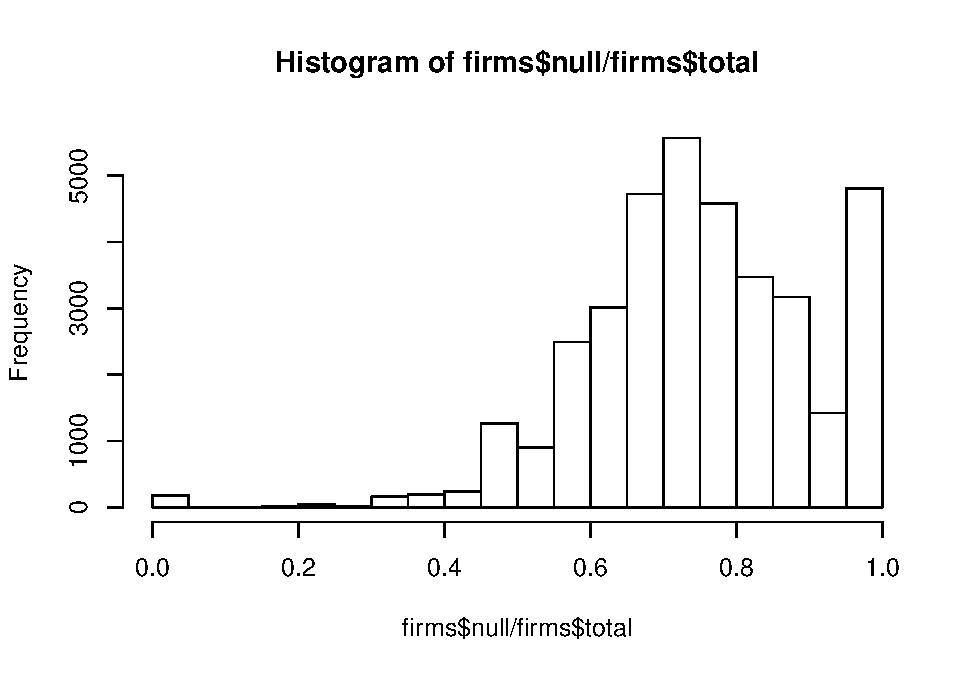
\includegraphics{TSLproject_files/figure-latex/unnamed-chunk-7-1.pdf}

\begin{Shaded}
\begin{Highlighting}[]
\CommentTok{# evaluate the distribution of all the sizes }
\CommentTok{# (log vs. ratio wrt total?)}
\KeywordTok{hist}\NormalTok{(}\KeywordTok{log}\NormalTok{(firms}\OperatorTok{$}\NormalTok{total))}
\end{Highlighting}
\end{Shaded}

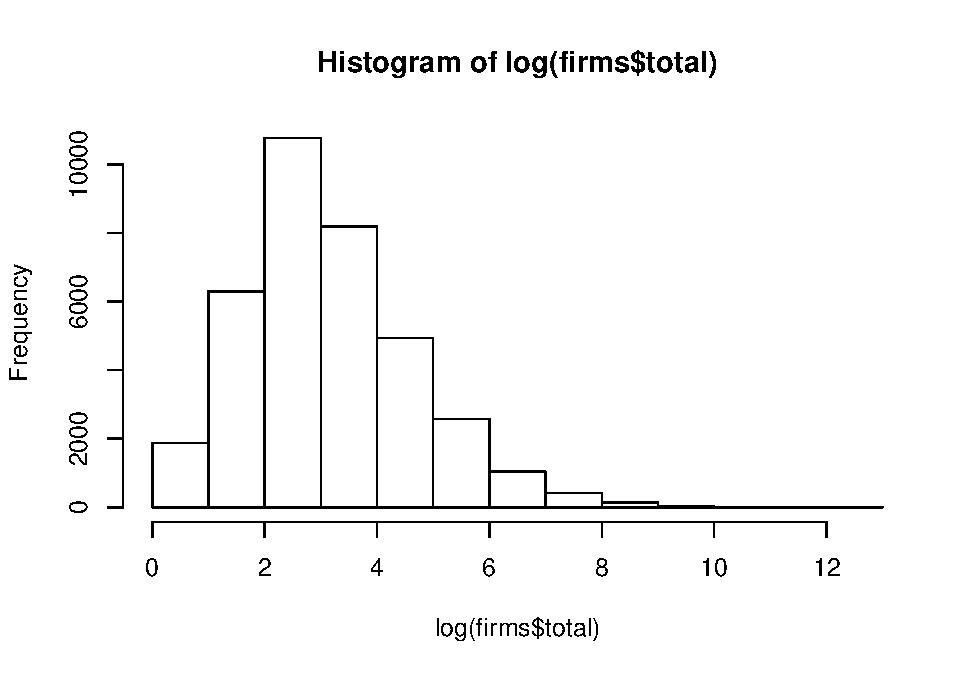
\includegraphics{TSLproject_files/figure-latex/unnamed-chunk-7-2.pdf}

\begin{Shaded}
\begin{Highlighting}[]
\KeywordTok{hist}\NormalTok{(}\KeywordTok{log}\NormalTok{(firms}\OperatorTok{$}\NormalTok{null))}
\end{Highlighting}
\end{Shaded}

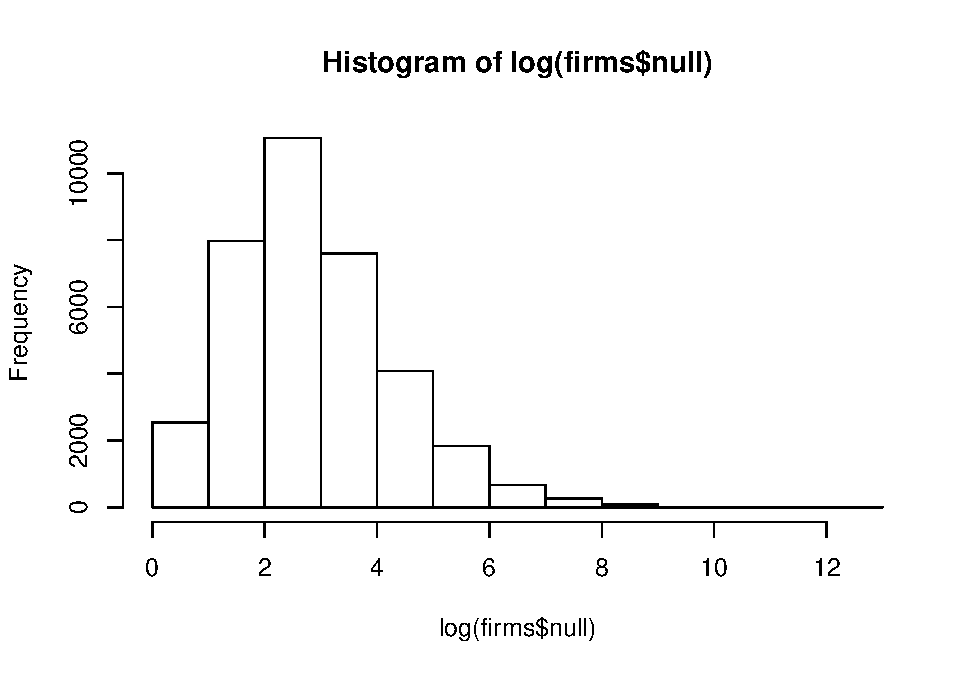
\includegraphics{TSLproject_files/figure-latex/unnamed-chunk-7-3.pdf}

\begin{Shaded}
\begin{Highlighting}[]
\KeywordTok{hist}\NormalTok{(}\KeywordTok{log}\NormalTok{(firms}\OperatorTok{$}\NormalTok{micro))}
\end{Highlighting}
\end{Shaded}

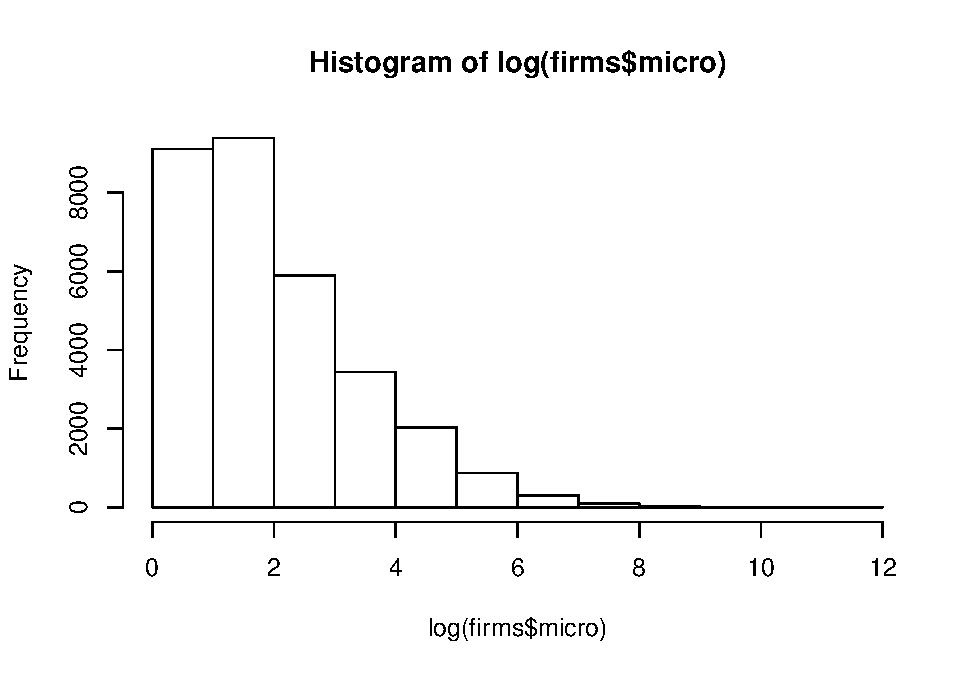
\includegraphics{TSLproject_files/figure-latex/unnamed-chunk-7-4.pdf}

\begin{Shaded}
\begin{Highlighting}[]
\KeywordTok{hist}\NormalTok{(firms}\OperatorTok{$}\NormalTok{micro}\OperatorTok{/}\NormalTok{firms}\OperatorTok{$}\NormalTok{total)}
\end{Highlighting}
\end{Shaded}

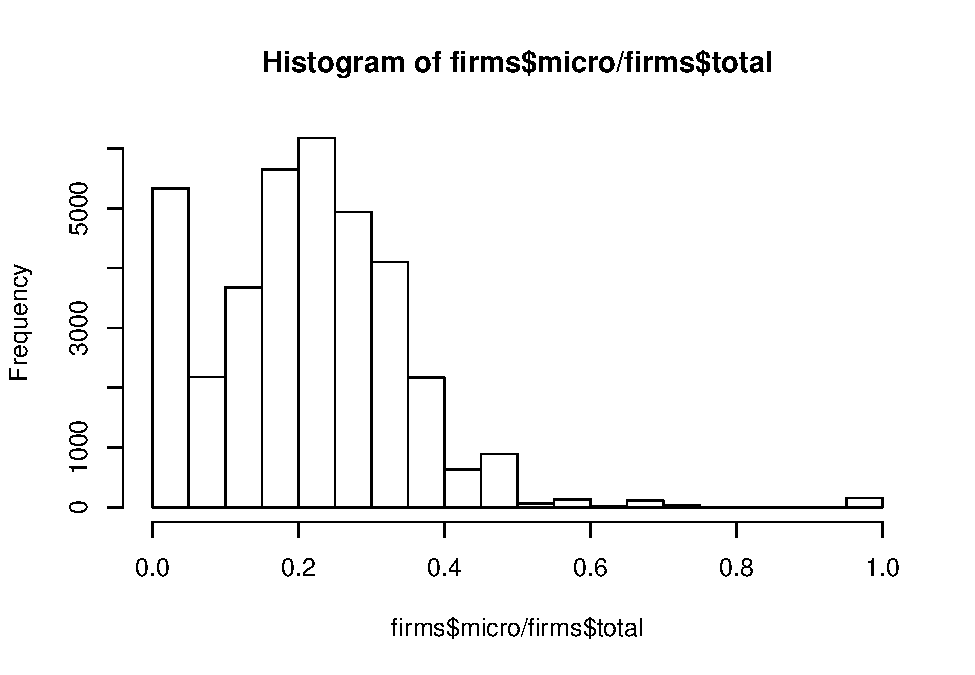
\includegraphics{TSLproject_files/figure-latex/unnamed-chunk-7-5.pdf}

\begin{Shaded}
\begin{Highlighting}[]
\KeywordTok{hist}\NormalTok{(}\KeywordTok{log}\NormalTok{(firms}\OperatorTok{$}\NormalTok{small))}
\end{Highlighting}
\end{Shaded}

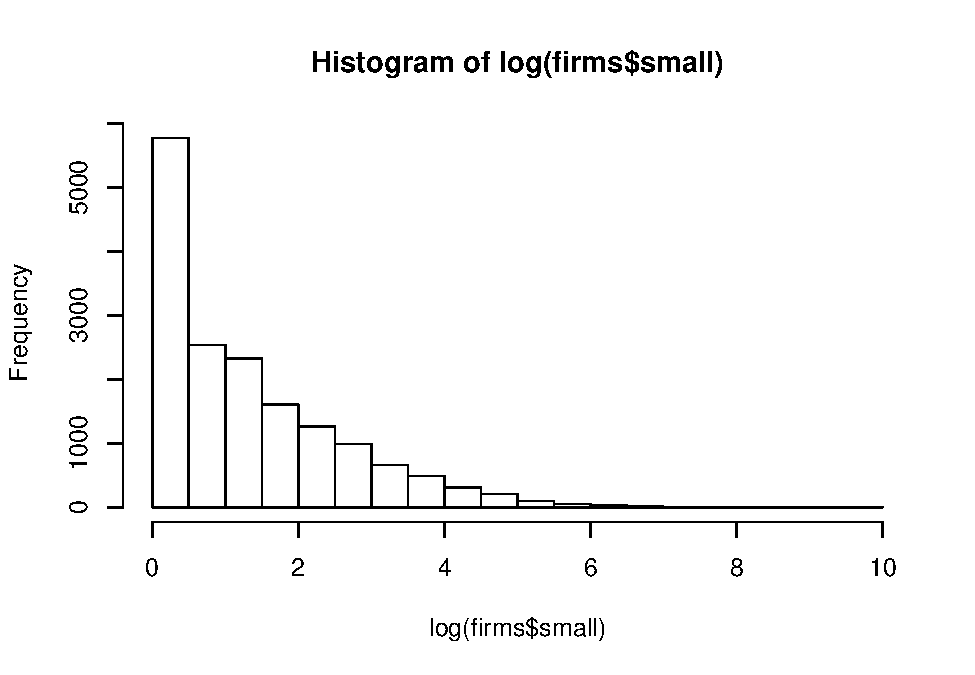
\includegraphics{TSLproject_files/figure-latex/unnamed-chunk-7-6.pdf}

\begin{Shaded}
\begin{Highlighting}[]
\KeywordTok{hist}\NormalTok{(firms}\OperatorTok{$}\NormalTok{small}\OperatorTok{/}\NormalTok{firms}\OperatorTok{$}\NormalTok{total)}
\end{Highlighting}
\end{Shaded}

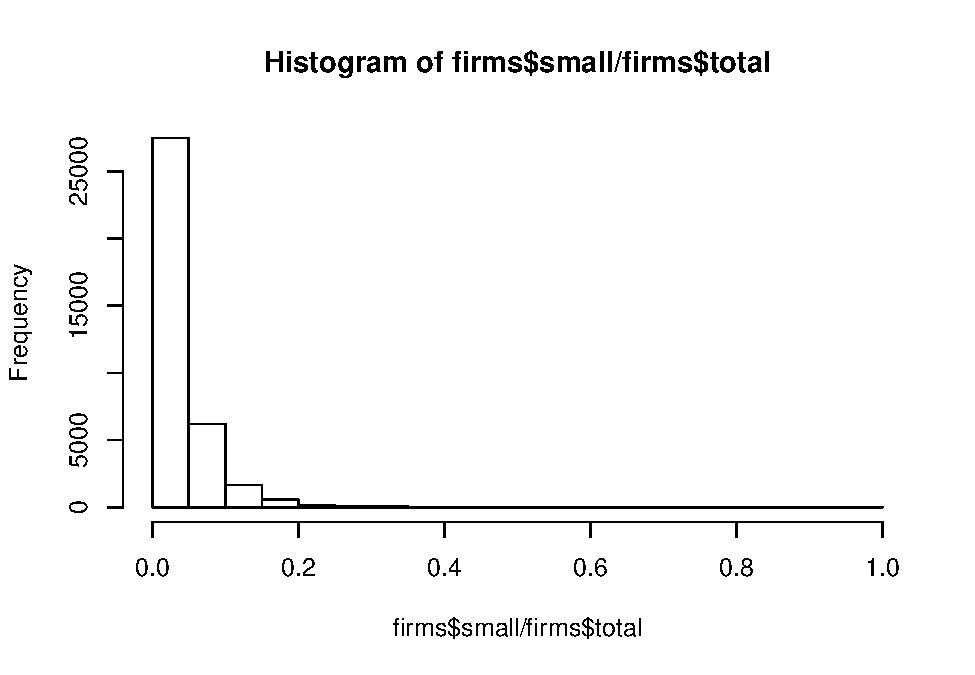
\includegraphics{TSLproject_files/figure-latex/unnamed-chunk-7-7.pdf}

\begin{Shaded}
\begin{Highlighting}[]
\KeywordTok{hist}\NormalTok{(}\KeywordTok{log}\NormalTok{(firms}\OperatorTok{$}\NormalTok{medium))}
\end{Highlighting}
\end{Shaded}

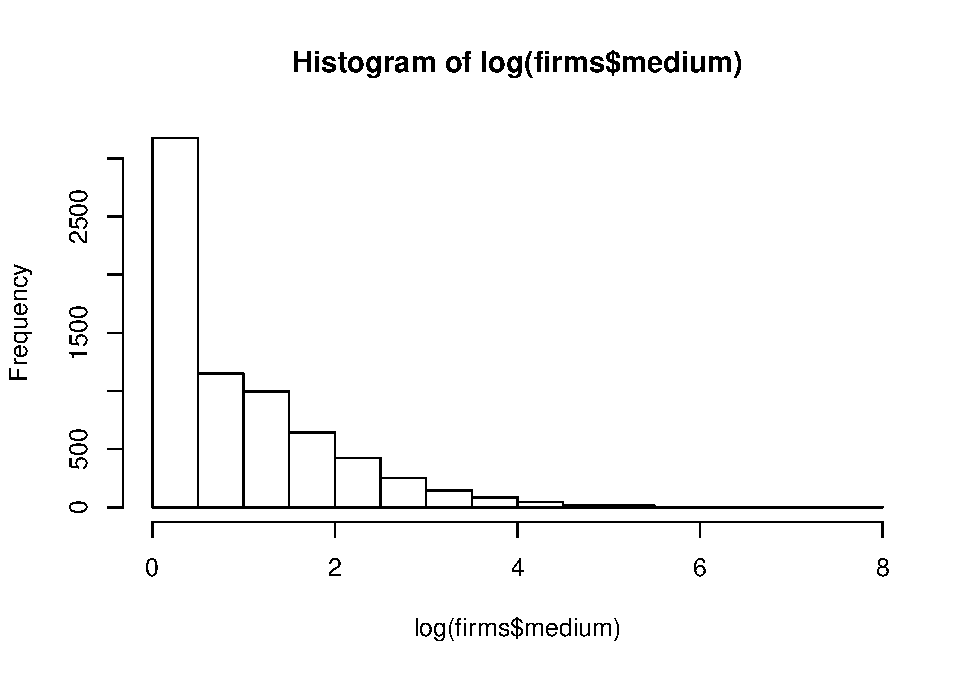
\includegraphics{TSLproject_files/figure-latex/unnamed-chunk-7-8.pdf}

\begin{Shaded}
\begin{Highlighting}[]
\KeywordTok{hist}\NormalTok{(firms}\OperatorTok{$}\NormalTok{medium}\OperatorTok{/}\NormalTok{firms}\OperatorTok{$}\NormalTok{total)}
\end{Highlighting}
\end{Shaded}

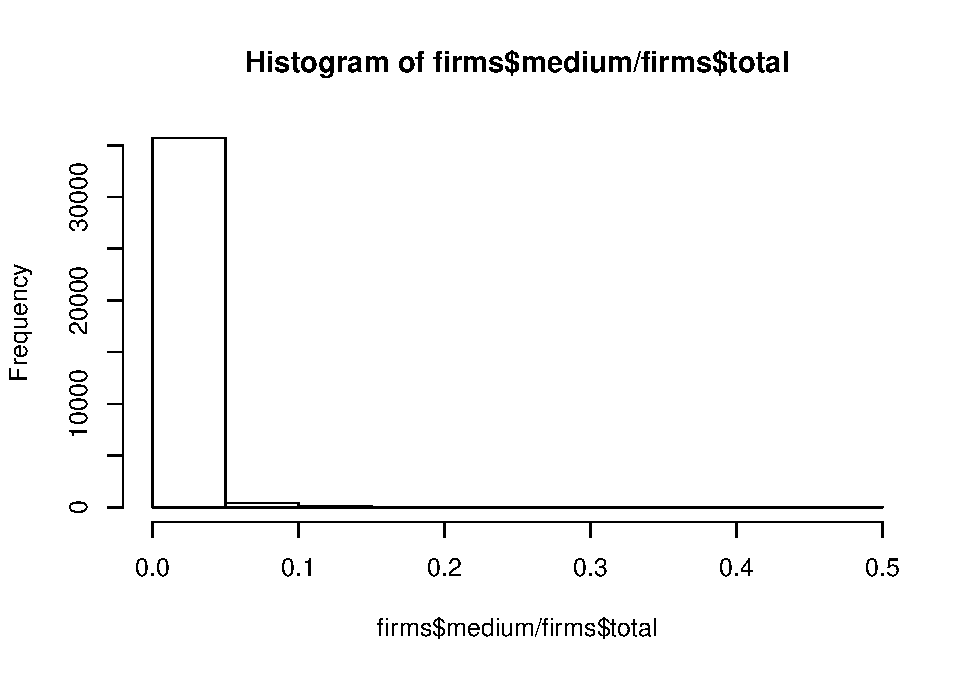
\includegraphics{TSLproject_files/figure-latex/unnamed-chunk-7-9.pdf}

\begin{Shaded}
\begin{Highlighting}[]
\KeywordTok{hist}\NormalTok{(}\KeywordTok{log}\NormalTok{(firms}\OperatorTok{$}\NormalTok{large))}
\end{Highlighting}
\end{Shaded}

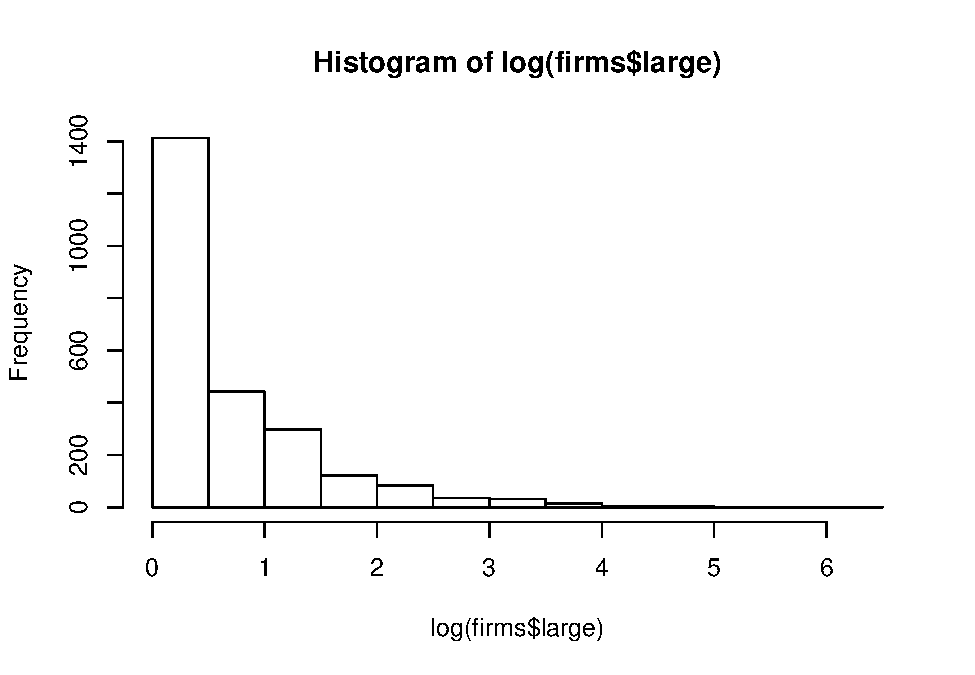
\includegraphics{TSLproject_files/figure-latex/unnamed-chunk-7-10.pdf}

\begin{Shaded}
\begin{Highlighting}[]
\KeywordTok{hist}\NormalTok{(firms}\OperatorTok{$}\NormalTok{large}\OperatorTok{/}\NormalTok{firms}\OperatorTok{$}\NormalTok{total)}
\end{Highlighting}
\end{Shaded}

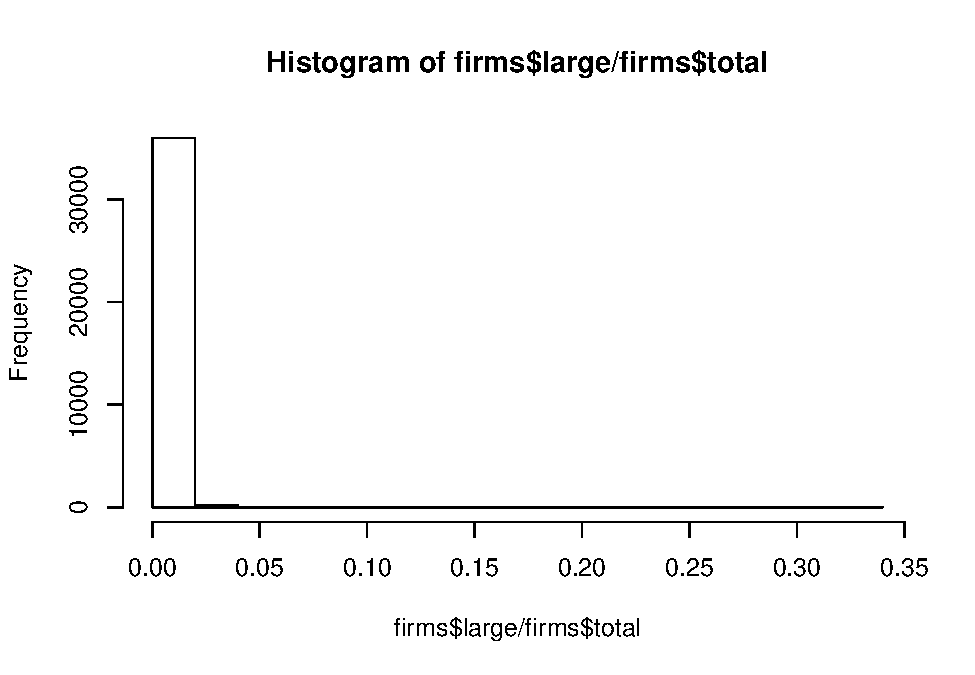
\includegraphics{TSLproject_files/figure-latex/unnamed-chunk-7-11.pdf}

\begin{Shaded}
\begin{Highlighting}[]
\CommentTok{# keep only logs?}
\end{Highlighting}
\end{Shaded}

PCA on firms data:

\begin{Shaded}
\begin{Highlighting}[]
\NormalTok{firms_clean <-}\StringTok{ }\NormalTok{firms[firms}\OperatorTok{$}\NormalTok{micro }\OperatorTok{<}\StringTok{ }\DecValTok{20000} \OperatorTok{&}\StringTok{ }\NormalTok{firms}\OperatorTok{$}\NormalTok{large }\OperatorTok{<}\StringTok{ }\DecValTok{200}\NormalTok{,]}
\NormalTok{myPr <-}\StringTok{ }\KeywordTok{prcomp}\NormalTok{(firms_clean[, }\DecValTok{4}\OperatorTok{:}\DecValTok{8}\NormalTok{], }\DataTypeTok{scale =} \OtherTok{TRUE}\NormalTok{)}
\CommentTok{#plot(scale(firms_clean$micro), scale(firms_clean$large))}
\CommentTok{#mean(firms_clean$micro)}
\CommentTok{#mean(firms_clean$large)}
\NormalTok{myPr}
\end{Highlighting}
\end{Shaded}

\begin{verbatim}
## Standard deviations (1, .., p=5):
## [1] 2.14610999 0.54465371 0.26631012 0.13983882 0.08419175
## 
## Rotation (n x k) = (5 x 5):
##              PC1         PC2         PC3        PC4         PC5
## micro  0.4533436  0.40064594 -0.03896827  0.3114187  0.73175293
## small  0.4605093  0.09419396  0.42164740  0.5486804 -0.54792511
## medium 0.4547148 -0.24046742  0.56534498 -0.6277884  0.14722974
## large  0.4207158 -0.75389742 -0.46725510  0.1841806  0.04885769
## null   0.4456943  0.45213319 -0.53174492 -0.4170461 -0.37450240
\end{verbatim}

\begin{Shaded}
\begin{Highlighting}[]
\KeywordTok{summary}\NormalTok{(myPr)}
\end{Highlighting}
\end{Shaded}

\begin{verbatim}
## Importance of components:
##                           PC1     PC2     PC3     PC4     PC5
## Standard deviation     2.1461 0.54465 0.26631 0.13984 0.08419
## Proportion of Variance 0.9212 0.05933 0.01418 0.00391 0.00142
## Cumulative Proportion  0.9212 0.98049 0.99467 0.99858 1.00000
\end{verbatim}

\begin{Shaded}
\begin{Highlighting}[]
\KeywordTok{plot}\NormalTok{(myPr, }\DataTypeTok{type =} \StringTok{"l"}\NormalTok{)}
\end{Highlighting}
\end{Shaded}

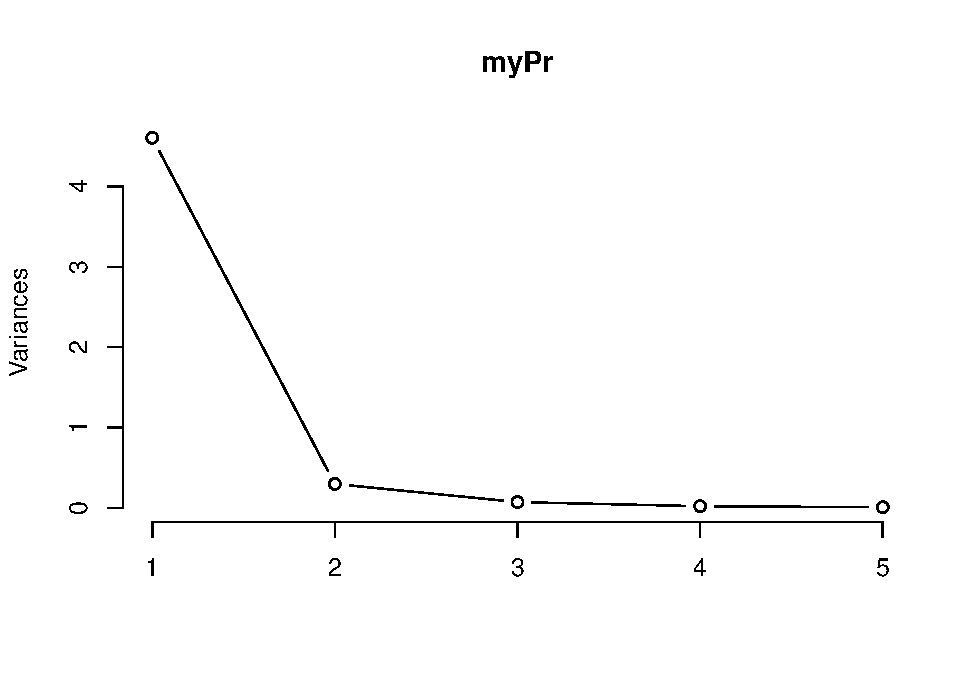
\includegraphics{TSLproject_files/figure-latex/unnamed-chunk-8-1.pdf}

\begin{Shaded}
\begin{Highlighting}[]
\KeywordTok{biplot}\NormalTok{(myPr, }\DataTypeTok{scale =} \DecValTok{0}\NormalTok{)}
\CommentTok{#extract PC scores...}
\KeywordTok{str}\NormalTok{(myPr)}
\end{Highlighting}
\end{Shaded}

\begin{verbatim}
## List of 5
##  $ sdev    : num [1:5] 2.1461 0.5447 0.2663 0.1398 0.0842
##  $ rotation: num [1:5, 1:5] 0.453 0.461 0.455 0.421 0.446 ...
##   ..- attr(*, "dimnames")=List of 2
##   .. ..$ : chr [1:5] "micro" "small" "medium" "large" ...
##   .. ..$ : chr [1:5] "PC1" "PC2" "PC3" "PC4" ...
##  $ center  : Named num [1:5] 30.026 5.648 1.003 0.204 74.926
##   ..- attr(*, "names")= chr [1:5] "micro" "small" "medium" "large" ...
##  $ scale   : Named num [1:5] 198.08 36.67 7.05 1.94 510.97
##   ..- attr(*, "names")= chr [1:5] "micro" "small" "medium" "large" ...
##  $ x       : num [1:36680, 1:5] -0.288 -0.304 3.043 -0.16 -0.31 ...
##   ..- attr(*, "dimnames")=List of 2
##   .. ..$ : chr [1:36680] "1" "2" "3" "4" ...
##   .. ..$ : chr [1:5] "PC1" "PC2" "PC3" "PC4" ...
##  - attr(*, "class")= chr "prcomp"
\end{verbatim}

\begin{Shaded}
\begin{Highlighting}[]
\CommentTok{#myPr$x #checking principal component scores}
\NormalTok{firms2 <-}\StringTok{ }\KeywordTok{cbind}\NormalTok{(firms_clean, myPr}\OperatorTok{$}\NormalTok{x[, }\DecValTok{1}\OperatorTok{:}\DecValTok{2}\NormalTok{])}
\KeywordTok{head}\NormalTok{(firms2)}
\end{Highlighting}
\end{Shaded}

\begin{verbatim}
##   CODGEO                    town total micro small medium large null
## 1   1001 L'Abergement-Clémenciat    25     3     0      0     0   22
## 2   1002   L'Abergement-de-Varey    10     1     0      0     0    9
## 3   1004       Ambérieu-en-Bugey   996   335    70     12     2  577
## 4   1005     Ambérieux-en-Dombes    99    23     3      0     0   73
## 5   1006                 Ambléon     4     0     0      0     0    4
## 6   1007                Ambronay   124    30     7      0     0   87
##          PC1          PC2
## 1 -0.2879301 -0.002515545
## 2 -0.3038468 -0.018063930
## 3  3.0434231  0.152878901
## 4 -0.1599969  0.090770640
## 5 -0.3104967 -0.024510834
## 6 -0.0815311  0.127591863
\end{verbatim}

\begin{Shaded}
\begin{Highlighting}[]
\CommentTok{#plot with ggplot...}
\KeywordTok{require}\NormalTok{(ggplot2)}
\end{Highlighting}
\end{Shaded}

\begin{verbatim}
## Loading required package: ggplot2
\end{verbatim}

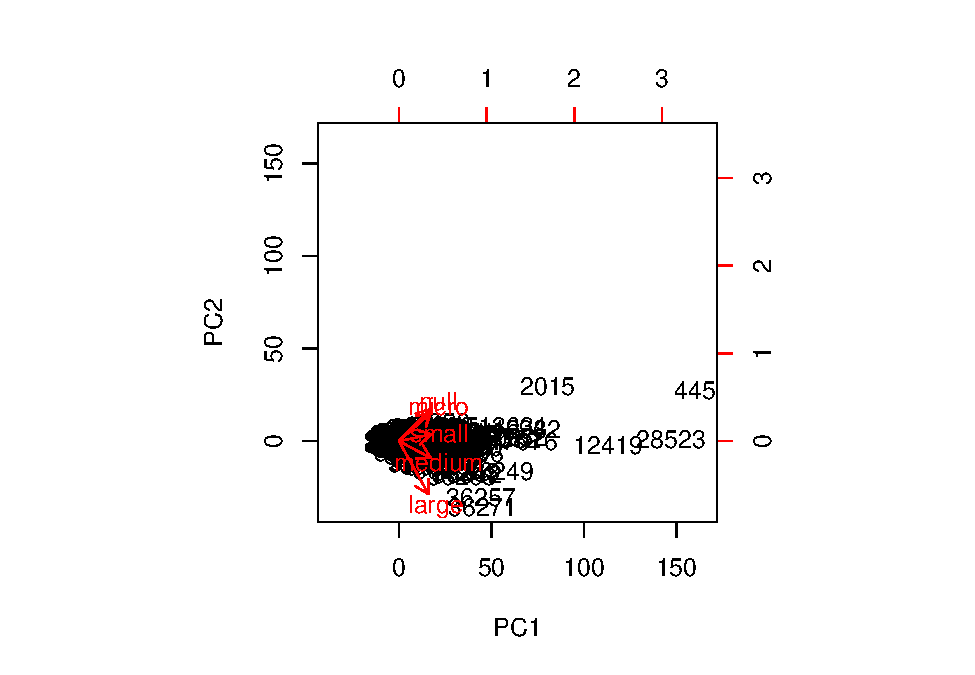
\includegraphics{TSLproject_files/figure-latex/unnamed-chunk-8-2.pdf}

\begin{Shaded}
\begin{Highlighting}[]
\KeywordTok{ggplot}\NormalTok{(firms2, }\KeywordTok{aes}\NormalTok{(PC1, PC2)) }\OperatorTok{+}\StringTok{ }
\StringTok{  }\KeywordTok{stat_ellipse}\NormalTok{(}\DataTypeTok{geom =} \StringTok{"polygon"}\NormalTok{, }\DataTypeTok{col =} \StringTok{"black"}\NormalTok{, }\DataTypeTok{alpha =} \FloatTok{0.5}\NormalTok{) }\OperatorTok{+}\StringTok{ }
\StringTok{  }\KeywordTok{geom_point}\NormalTok{(}\DataTypeTok{shape =} \DecValTok{21}\NormalTok{, }\DataTypeTok{col =} \StringTok{"black"}\NormalTok{)}
\end{Highlighting}
\end{Shaded}

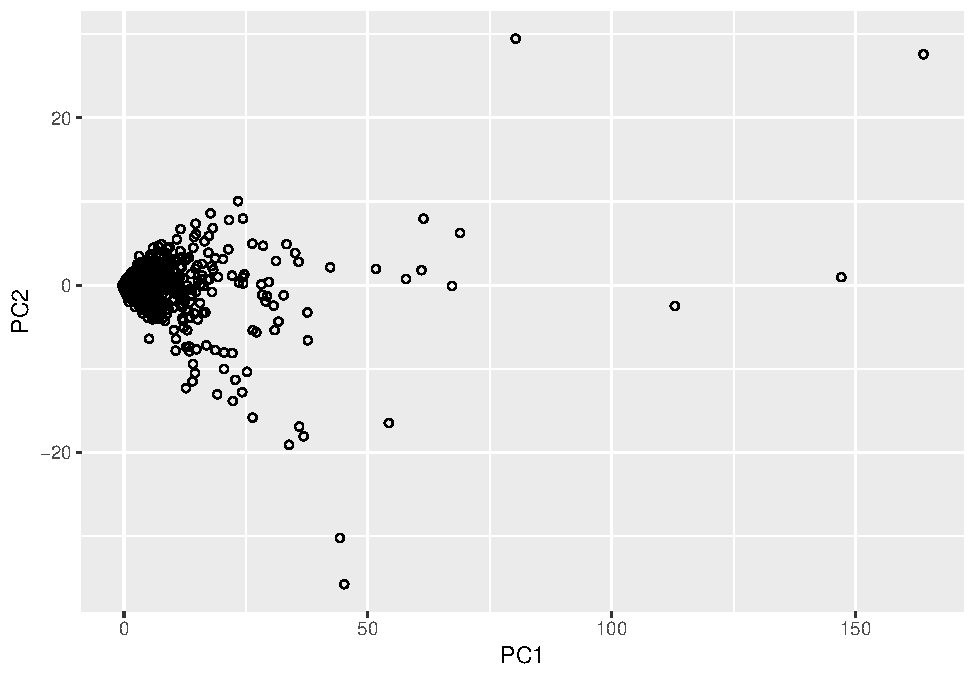
\includegraphics{TSLproject_files/figure-latex/unnamed-chunk-8-3.pdf}

\begin{Shaded}
\begin{Highlighting}[]
\CommentTok{# correlations between variables and PCs...}
\KeywordTok{cor}\NormalTok{(firms_clean[, }\DecValTok{4}\OperatorTok{:}\DecValTok{8}\NormalTok{], firms2[,}\DecValTok{9}\OperatorTok{:}\DecValTok{10}\NormalTok{])}
\end{Highlighting}
\end{Shaded}

\begin{verbatim}
##              PC1         PC2
## micro  0.9729251  0.21821330
## small  0.9883037  0.05130309
## medium 0.9758680 -0.13097147
## large  0.9029024 -0.41061303
## null   0.9565091  0.24625602
\end{verbatim}

\subsection{What we have learned}\label{what-we-have-learned}

\begin{itemize}
\tightlist
\item
  More micro firms than small ones
\item
  \ldots{}
\end{itemize}

\subsection{How to use these data}\label{how-to-use-these-data}

We plan to use these for the following tasks:

\begin{itemize}
\tightlist
\item
  predict the salaries using such information as proxy for the
  competition in the job market;
\item
  predict the total number of firms, using salary data;
\item
  geo-spatial plot for firms' size
\item
  \ldots{}
\end{itemize}

\section{Analyze geographical data}\label{analyze-geographical-data}

\subsection{Pre-processing}\label{pre-processing-1}

\begin{Shaded}
\begin{Highlighting}[]
\CommentTok{# preliminary checks}
\KeywordTok{dim}\NormalTok{(geo)}
\end{Highlighting}
\end{Shaded}

\begin{verbatim}
## [1] 36840     8
\end{verbatim}

\begin{Shaded}
\begin{Highlighting}[]
\KeywordTok{names}\NormalTok{(geo)}
\end{Highlighting}
\end{Shaded}

\begin{verbatim}
## [1] "region"         "region_capital" "department"     "town_name"     
## [5] "postal_code"    "CODGEO"         "latitude"       "longitude"
\end{verbatim}

\begin{Shaded}
\begin{Highlighting}[]
\KeywordTok{head}\NormalTok{(geo)}
\end{Highlighting}
\end{Shaded}

\begin{verbatim}
##        region region_capital department            town_name postal_code
## 1 Rhône-Alpes           Lyon        Ain             Attignat       01340
## 2 Rhône-Alpes           Lyon        Ain             Beaupont       01270
## 3 Rhône-Alpes           Lyon        Ain                 Bény       01370
## 4 Rhône-Alpes           Lyon        Ain            Béreyziat       01340
## 5 Rhône-Alpes           Lyon        Ain Bohas-Meyriat-Rignat       01250
## 6 Rhône-Alpes           Lyon        Ain      Bourg-en-Bresse       01000
##   CODGEO latitude longitude
## 1   1024 46.28333  5.166667
## 2   1029 46.40000  5.266667
## 3   1038 46.33333  5.283333
## 4   1040 46.36667      5.05
## 5   1245 46.13333       5.4
## 6   1053 46.20000  5.216667
\end{verbatim}

\begin{Shaded}
\begin{Highlighting}[]
\KeywordTok{str}\NormalTok{(geo)}
\end{Highlighting}
\end{Shaded}

\begin{verbatim}
## 'data.frame':    36840 obs. of  8 variables:
##  $ region        : Factor w/ 28 levels "Alsace","Aquitaine",..: 27 27 27 27 27 27 27 27 27 27 ...
##  $ region_capital: Factor w/ 28 levels "Ajaccio","Amiens",..: 14 14 14 14 14 14 14 14 14 14 ...
##  $ department    : Factor w/ 102 levels "Ain","Aisne",..: 1 1 1 1 1 1 1 1 1 1 ...
##  $ town_name     : Factor w/ 34142 levels "Aast","Abainville",..: 1264 2487 2798 2821 3515 4001 4708 5689 5730 6645 ...
##  $ postal_code   : Factor w/ 6106 levels "01000","01090",..: 26 19 29 26 17 1 23 16 17 17 ...
##  $ CODGEO        : int  1024 1029 1038 1040 1245 1053 1065 1069 1072 1095 ...
##  $ latitude      : num  46.3 46.4 46.3 46.4 46.1 ...
##  $ longitude     : Factor w/ 1151 levels "","-","-0,75",..: 874 880 881 864 891 877 872 880 885 892 ...
\end{verbatim}

\begin{Shaded}
\begin{Highlighting}[]
\KeywordTok{summary}\NormalTok{(geo)}
\end{Highlighting}
\end{Shaded}

\begin{verbatim}
##            region       region_capital           department   
##  Midi-Pyrénées: 3028   Toulouse: 3028   Pas-de-Calais :  898  
##  Rhône-Alpes  : 2890   Lyon    : 2890   Aisne         :  816  
##  Lorraine     : 2336   Metz    : 2336   Somme         :  783  
##  Aquitaine    : 2300   Bordeaux: 2300   Seine-Maritime:  747  
##  Picardie     : 2295   Amiens  : 2295   Moselle       :  732  
##  Bourgogne    : 2050   Dijon   : 2050   Côte-d'Or     :  709  
##  (Other)      :21941   (Other) :21941   (Other)       :32155  
##           town_name      postal_code        CODGEO         latitude    
##  Paris         :   21   51300  :   46   Min.   : 1001   Min.   :41.39  
##  Sainte-Colombe:   14   51800  :   44   1st Qu.:24577   1st Qu.:45.22  
##  Saint-Sauveur :   12   70000  :   42   Median :48191   Median :47.43  
##  Beaulieu      :   11   88500  :   42   Mean   :46298   Mean   :47.00  
##  Saint-Sulpice :   11   80140  :   40   3rd Qu.:67043   3rd Qu.:48.85  
##  Sainte-Marie  :   11   02160  :   38   Max.   :97617   Max.   :51.08  
##  (Other)       :36760   (Other):36588                   NA's   :2929   
##     longitude    
##          : 2841  
##  2.433333:  105  
##  2.333333:  100  
##  1.833333:   99  
##  2.116667:   98  
##  2.25    :   94  
##  (Other) :33503
\end{verbatim}

\begin{Shaded}
\begin{Highlighting}[]
\CommentTok{# spot "," instead of "." in longitude}
\NormalTok{newLong       <-}\StringTok{ }\KeywordTok{as.character}\NormalTok{(geo}\OperatorTok{$}\NormalTok{longitude)    }\CommentTok{# copy the vector}
\KeywordTok{sum}\NormalTok{(}\KeywordTok{grep}\NormalTok{(}\StringTok{","}\NormalTok{, newLong))                         }\CommentTok{# total commas}
\end{Highlighting}
\end{Shaded}

\begin{verbatim}
## [1] 994302
\end{verbatim}

\begin{Shaded}
\begin{Highlighting}[]
\NormalTok{ind_long_err  <-}\StringTok{ }\KeywordTok{grep}\NormalTok{(}\StringTok{","}\NormalTok{, newLong)             }\CommentTok{# indexing them}
\NormalTok{newLong       <-}\StringTok{ }\KeywordTok{gsub}\NormalTok{(}\StringTok{","}\NormalTok{, }\StringTok{"."}\NormalTok{, newLong)        }\CommentTok{# substituting them with dots}
\NormalTok{indNA_Long    <-}\StringTok{ }\KeywordTok{is.na}\NormalTok{(}\KeywordTok{as.numeric}\NormalTok{((newLong)))   }\CommentTok{# spot NA}
\end{Highlighting}
\end{Shaded}

\begin{verbatim}
## Warning: si è prodotto un NA per coercizione
\end{verbatim}

\begin{Shaded}
\begin{Highlighting}[]
\NormalTok{geo}\OperatorTok{$}\NormalTok{longitude[indNA_Long]                       }\CommentTok{# verify that they were actually missing}
\end{Highlighting}
\end{Shaded}

\begin{verbatim}
##    [1]                                                                    
##   [35]                                                                    
##   [69]                                                                    
##  [103]                                                                    
##  [137]                                                                    
##  [171]                                                                    
##  [205]                                                                    
##  [239]                                                                    
##  [273]                                                                    
##  [307]                                                                    
##  [341]                                                                    
##  [375] -             -   -         -   -                                  
##  [409]                                                                    
##  [443]               -             -         -         -                  
##  [477]   -     - -             -       -                                  
##  [511]                                                                    
##  [545]                                                                    
##  [579]                                                                    
##  [613]                                                                    
##  [647]                                                                    
##  [681]                                                                    
##  [715]                                                                    
##  [749]                                                                    
##  [783]                                                                    
##  [817]                                                                    
##  [851]                                                                    
##  [885]                                                                    
##  [919]                                                                    
##  [953]                                                                    
##  [987]                                                 -                  
## [1021]   -                   -           -                                
## [1055]                                 -                 - -           -  
## [1089] - -         -       -                               -              
## [1123]                                                                    
## [1157]                                                                    
## [1191]                                                                    
## [1225]                                                                    
## [1259]                                               -                    
## [1293]                                                                    
## [1327]                                                                    
## [1361]                                                                    
## [1395]                                                                    
## [1429]                                     - - -                          
## [1463]                                                                    
## [1497]                                                                    
## [1531]                                                                    
## [1565]                                                                    
## [1599]                                                                    
## [1633]                                                                    
## [1667]                                                                    
## [1701]                                                                    
## [1735]                                                                    
## [1769]                                                                    
## [1803]                                                                    
## [1837]                                                                    
## [1871]                                                             -   -  
## [1905]     -                               -   -       -           -      
## [1939]                                                                    
## [1973]                                                                    
## [2007]                                     -                              
## [2041]                                                               - - -
## [2075] -     - - - -   -           - -   - -   - - -                      
## [2109]                                                                    
## [2143]                                                                    
## [2177]                                                                    
## [2211]                                                                    
## [2245]                                                                    
## [2279]                       - -     -                                    
## [2313]                                                                    
## [2347]                                                                    
## [2381]                                                                    
## [2415]                                                                    
## [2449]                                                   -           -   -
## [2483]                                                                    
## [2517]                                                                    
## [2551]                                                                    
## [2585]                                                                    
## [2619]                                                                    
## [2653]         -                       -                 -                
## [2687]                                                                    
## [2721]                                                                    
## [2755]                                                                    
## [2789]                                                                    
## [2823]                                                                    
## [2857]                                                                    
## [2891]                              
## 1151 Levels:  - -0,75 -0.008333 -0.016667 -0.01679 -0.025 ... 9.516667
\end{verbatim}

\begin{Shaded}
\begin{Highlighting}[]
\NormalTok{geo}\OperatorTok{$}\NormalTok{longitude <-}\StringTok{ }\KeywordTok{as.numeric}\NormalTok{(newLong)            }\CommentTok{# overwrite the longitude variable with the new one}
\end{Highlighting}
\end{Shaded}

\begin{verbatim}
## Warning: si è prodotto un NA per coercizione
\end{verbatim}

\begin{Shaded}
\begin{Highlighting}[]
\CommentTok{# Check for duplicated data (e.g., cities with different postal codes, that we dropped):}
  \CommentTok{# es. to verify it:  try on the initial dataset}
  \CommentTok{# sum(geo$nom_commune == "Paris")}
  \CommentTok{# ind_duplic <- geo$nom_commune == "Paris"}
  \CommentTok{# geo[ind_duplic,]}
\KeywordTok{sum}\NormalTok{(}\KeywordTok{duplicated.data.frame}\NormalTok{(geo)) }
\end{Highlighting}
\end{Shaded}

\begin{verbatim}
## [1] 117
\end{verbatim}

\begin{Shaded}
\begin{Highlighting}[]
\CommentTok{# retaing unique postal cities}
\NormalTok{geo <-}\StringTok{ }\KeywordTok{unique}\NormalTok{(geo, }\DataTypeTok{by =} \StringTok{"CODGEO"}\NormalTok{)}

\CommentTok{# check again}
\KeywordTok{head}\NormalTok{(geo)}
\end{Highlighting}
\end{Shaded}

\begin{verbatim}
##        region region_capital department            town_name postal_code
## 1 Rhône-Alpes           Lyon        Ain             Attignat       01340
## 2 Rhône-Alpes           Lyon        Ain             Beaupont       01270
## 3 Rhône-Alpes           Lyon        Ain                 Bény       01370
## 4 Rhône-Alpes           Lyon        Ain            Béreyziat       01340
## 5 Rhône-Alpes           Lyon        Ain Bohas-Meyriat-Rignat       01250
## 6 Rhône-Alpes           Lyon        Ain      Bourg-en-Bresse       01000
##   CODGEO latitude longitude
## 1   1024 46.28333  5.166667
## 2   1029 46.40000  5.266667
## 3   1038 46.33333  5.283333
## 4   1040 46.36667  5.050000
## 5   1245 46.13333  5.400000
## 6   1053 46.20000  5.216667
\end{verbatim}

\begin{Shaded}
\begin{Highlighting}[]
\KeywordTok{summary}\NormalTok{(geo)}
\end{Highlighting}
\end{Shaded}

\begin{verbatim}
##            region       region_capital           department   
##  Midi-Pyrénées: 3021   Toulouse: 3021   Pas-de-Calais :  894  
##  Rhône-Alpes  : 2882   Lyon    : 2882   Aisne         :  816  
##  Lorraine     : 2333   Metz    : 2333   Somme         :  782  
##  Aquitaine    : 2296   Bordeaux: 2296   Seine-Maritime:  745  
##  Picardie     : 2291   Amiens  : 2291   Moselle       :  730  
##  Bourgogne    : 2046   Dijon   : 2046   Côte-d'Or     :  707  
##  (Other)      :21854   (Other) :21854   (Other)       :32049  
##           town_name      postal_code        CODGEO         latitude    
##  Paris         :   19   51300  :   46   Min.   : 1001   Min.   :41.39  
##  Sainte-Colombe:   14   51800  :   44   1st Qu.:24562   1st Qu.:45.22  
##  Saint-Sauveur :   12   70000  :   42   Median :48180   Median :47.43  
##  Beaulieu      :   11   88500  :   42   Mean   :46276   Mean   :47.00  
##  Saint-Sulpice :   11   80140  :   40   3rd Qu.:67037   3rd Qu.:48.85  
##  Sainte-Marie  :   11   02160  :   38   Max.   :97617   Max.   :51.08  
##  (Other)       :36645   (Other):36471                   NA's   :2925   
##    longitude      
##  Min.   :-5.1000  
##  1st Qu.: 0.6833  
##  Median : 2.6167  
##  Mean   : 2.7329  
##  3rd Qu.: 4.8500  
##  Max.   : 9.5167  
##  NA's   :2903
\end{verbatim}

Assign lat and long values for NAs units:

\begin{Shaded}
\begin{Highlighting}[]
\KeywordTok{require}\NormalTok{(ggmap)}
\end{Highlighting}
\end{Shaded}

\begin{verbatim}
## Loading required package: ggmap
\end{verbatim}

\begin{Shaded}
\begin{Highlighting}[]
\CommentTok{# [ delete? ]}
\CommentTok{# # compare numbers of NA in latitude and longitude }
\CommentTok{# sum(is.na(geo$latitude)) - sum(is.na(geo$longitude))}
\CommentTok{# # check if they match or not}
\CommentTok{# sum(!is.na(geo$latitude[indNA_Long]))}
\CommentTok{# # 64 obs are missing in longitude but not in latitude, hence 88 vice versa}

\CommentTok{# index of NAs and their total}
\NormalTok{indNA_coord =}\StringTok{ }\KeywordTok{is.na}\NormalTok{(geo}\OperatorTok{$}\NormalTok{latitude) }\OperatorTok{|}\StringTok{ }\KeywordTok{is.na}\NormalTok{(geo}\OperatorTok{$}\NormalTok{longitude)}
\KeywordTok{sum}\NormalTok{(indNA_coord)}
\end{Highlighting}
\end{Shaded}

\begin{verbatim}
## [1] 2989
\end{verbatim}

\begin{Shaded}
\begin{Highlighting}[]
\CommentTok{# NO MORE NEEDED BECAUSE IS A CSV FILE}
    \CommentTok{# # initialize variables}
    \CommentTok{# city_search = 0}
    \CommentTok{# res = as.data.frame(matrix(c(0, 0, 0), 1, 3))}
    \CommentTok{# names(res) = c("lon", "lat", "address")}
    \CommentTok{# }
    \CommentTok{# # retrieve lat and long (Google API = 2500 request per day)}
    \CommentTok{# # my_iter = floor(sum(indNA_coord)/3)}
    \CommentTok{# for (i in 1:sum(indNA_coord))\{}
    \CommentTok{# }
    \CommentTok{#   # city searched}
    \CommentTok{#   city_search[i] = paste(c(as.character(NA_coord$town_name[i]), as.character(NA_coord$postal_code[i]), as.character(NA_coord$department[i]), "France"), sep=" ", collapse = ", ")}
    \CommentTok{#   }
    \CommentTok{#   # solution}
    \CommentTok{#   res[i,] = geocode(city_search[i], output = "latlona", source = c("google", "dsk"), messaging = FALSE)}
    \CommentTok{# }
    \CommentTok{#   # retrieve still missing data, because of existing problems with API (up to 15 trials)}
    \CommentTok{#   j = 0}
    \CommentTok{#   while (any(is.na(res[i,])) & j < 25)\{}
    \CommentTok{#     res[i,] = geocode(city_search[i], output = "latlona", source = c("google", "dsk"), messaging = FALSE)}
    \CommentTok{#     j = j + 1}
    \CommentTok{#   \}}
    \CommentTok{# \}}

    \CommentTok{# # check the solution}
    \CommentTok{# sol = cbind(searched = city_search, res)}

    \CommentTok{# # save it as a csv file to save time}
    \CommentTok{# write.csv(retrieved_geo_NA[,2:3], "geo_NA_Final.csv", quote = FALSE, row.names=FALSE, fileEncoding = "UTF-8")}
    

\CommentTok{# read the created csv}
\NormalTok{retrieved_geo_NA =}\StringTok{ }\KeywordTok{read.csv}\NormalTok{(}\StringTok{"geo_NA_Final.csv"}\NormalTok{, }\DataTypeTok{header =}\NormalTok{ T, }\DataTypeTok{encoding =} \StringTok{"UTF-8"}\NormalTok{)}
\CommentTok{# get only long and lat and assign to original NA }
\NormalTok{geo}\OperatorTok{$}\NormalTok{latitude[indNA_coord] =}\StringTok{ }\NormalTok{retrieved_geo_NA[,}\DecValTok{2}\NormalTok{]}
\NormalTok{geo}\OperatorTok{$}\NormalTok{longitude[indNA_coord] =}\StringTok{ }\NormalTok{retrieved_geo_NA[,}\DecValTok{1}\NormalTok{]}

\CommentTok{# there are 37 still missing units, which are towns located in old colonies far from Europe}
\NormalTok{indNA_coord =}\StringTok{ }\KeywordTok{is.na}\NormalTok{(geo}\OperatorTok{$}\NormalTok{latitude) }\OperatorTok{|}\StringTok{ }\KeywordTok{is.na}\NormalTok{(geo}\OperatorTok{$}\NormalTok{longitude)}
\KeywordTok{sum}\NormalTok{(indNA_coord)}
\end{Highlighting}
\end{Shaded}

\begin{verbatim}
## [1] 37
\end{verbatim}

\begin{Shaded}
\begin{Highlighting}[]
\CommentTok{# exclude those towns}
\NormalTok{geo =}\StringTok{ }\NormalTok{geo[}\OperatorTok{!}\NormalTok{indNA_coord,]}

\KeywordTok{summary}\NormalTok{(geo)}
\end{Highlighting}
\end{Shaded}

\begin{verbatim}
##            region       region_capital           department   
##  Midi-Pyrénées: 3021   Toulouse: 3021   Pas-de-Calais :  894  
##  Rhône-Alpes  : 2882   Lyon    : 2882   Aisne         :  816  
##  Lorraine     : 2333   Metz    : 2333   Somme         :  782  
##  Aquitaine    : 2296   Bordeaux: 2296   Seine-Maritime:  745  
##  Picardie     : 2291   Amiens  : 2291   Moselle       :  730  
##  Bourgogne    : 2046   Dijon   : 2046   Côte-d'Or     :  707  
##  (Other)      :21817   (Other) :21817   (Other)       :32012  
##           town_name      postal_code        CODGEO         latitude     
##  Paris         :   19   51300  :   46   Min.   : 1001   Min.   :-21.38  
##  Sainte-Colombe:   14   51800  :   44   1st Qu.:24551   1st Qu.: 45.15  
##  Saint-Sauveur :   12   70000  :   42   Median :48162   Median : 47.38  
##  Beaulieu      :   11   88500  :   42   Mean   :46224   Mean   : 46.87  
##  Saint-Sulpice :   11   80140  :   40   3rd Qu.:67006   3rd Qu.: 48.83  
##  Sainte-Marie  :   11   02160  :   38   Max.   :97611   Max.   : 51.08  
##  (Other)       :36608   (Other):36434                                   
##    longitude       
##  Min.   :-63.0885  
##  1st Qu.:  0.6667  
##  Median :  2.6333  
##  Mean   :  2.6617  
##  3rd Qu.:  4.8667  
##  Max.   : 55.8250  
## 
\end{verbatim}

\subsection{EDA}\label{eda-1}

\begin{Shaded}
\begin{Highlighting}[]
\CommentTok{#install.packages("ggplot2")}
\CommentTok{#install.packages("ggmap")}
\KeywordTok{require}\NormalTok{(ggplot2)}
\KeywordTok{require}\NormalTok{(ggmap)}

\CommentTok{# plot france (center: 2.213749 46.227638)}
\CommentTok{# fra_center = as.numeric(geocode("France"))}
\NormalTok{fra_center =}\StringTok{ }\KeywordTok{c}\NormalTok{(}\FloatTok{2.213749}\NormalTok{, }\FloatTok{46.227638}\NormalTok{)}
\NormalTok{FraMap =}\StringTok{ }\KeywordTok{ggmap}\NormalTok{(}\KeywordTok{get_googlemap}\NormalTok{(}\DataTypeTok{center=}\NormalTok{fra_center, }\DataTypeTok{scale=}\DecValTok{2}\NormalTok{, }\DataTypeTok{zoom=}\DecValTok{5}\NormalTok{), }\DataTypeTok{extent=}\StringTok{"normal"}\NormalTok{)}
\end{Highlighting}
\end{Shaded}

\begin{verbatim}
## Map from URL : http://maps.googleapis.com/maps/api/staticmap?center=46.227638,2.213749&zoom=5&size=640x640&scale=2&maptype=terrain&sensor=false
\end{verbatim}

\begin{Shaded}
\begin{Highlighting}[]
\NormalTok{FraMap}
\end{Highlighting}
\end{Shaded}

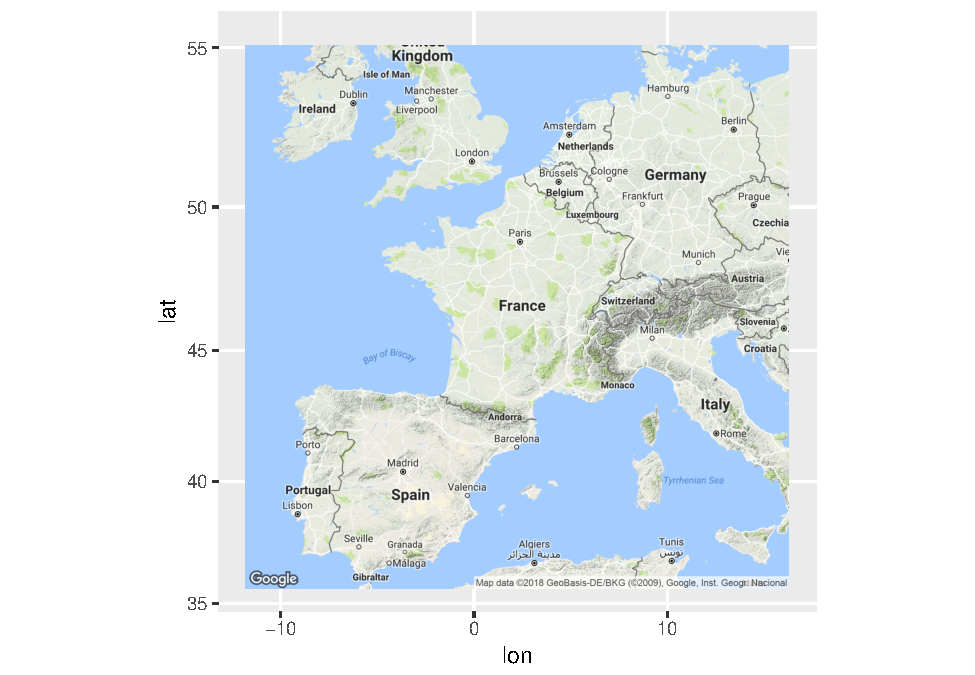
\includegraphics{TSLproject_files/figure-latex/unnamed-chunk-11-1.pdf}

\begin{Shaded}
\begin{Highlighting}[]
\CommentTok{# plot all towns available}
\NormalTok{geo_pos =}\StringTok{ }\KeywordTok{as.data.frame}\NormalTok{(}\KeywordTok{cbind}\NormalTok{(}\DataTypeTok{lon =}\NormalTok{ geo}\OperatorTok{$}\NormalTok{longitude, }\DataTypeTok{lat =}\NormalTok{ geo}\OperatorTok{$}\NormalTok{latitude))}
\NormalTok{geo_pos =}\StringTok{ }\NormalTok{geo_pos[}\KeywordTok{complete.cases}\NormalTok{(geo_pos),]}
\NormalTok{FraMap }\OperatorTok{+}
\StringTok{  }\KeywordTok{geom_point}\NormalTok{(}\KeywordTok{aes}\NormalTok{(}\DataTypeTok{x=}\NormalTok{lon, }\DataTypeTok{y=}\NormalTok{lat), }\DataTypeTok{data=}\NormalTok{geo_pos, }\DataTypeTok{col=}\StringTok{"orange"}\NormalTok{, }\DataTypeTok{alpha=}\FloatTok{0.1}\NormalTok{) }
\end{Highlighting}
\end{Shaded}

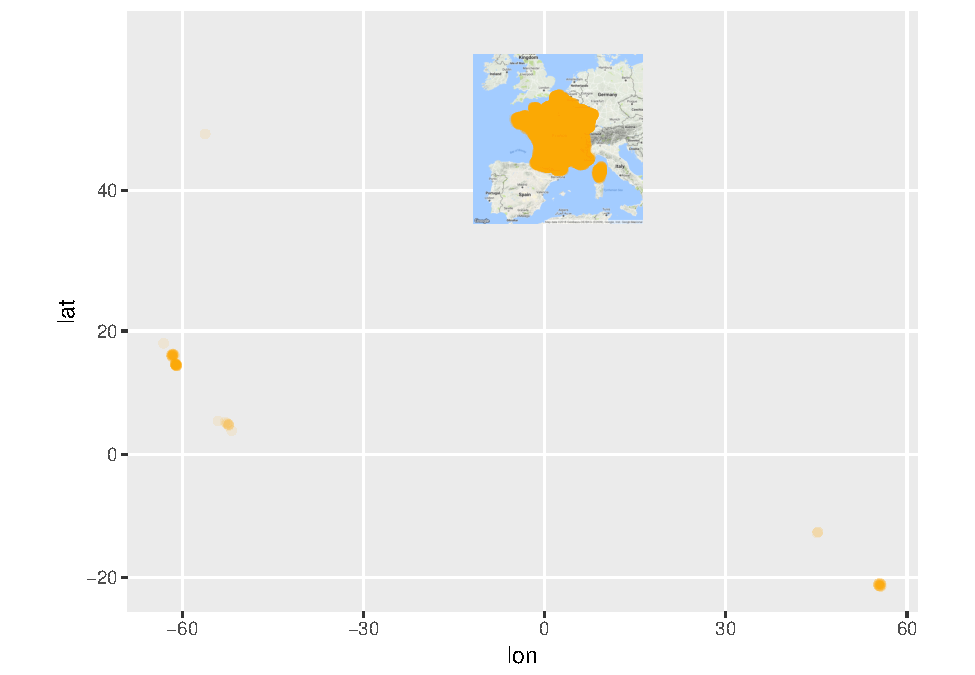
\includegraphics{TSLproject_files/figure-latex/unnamed-chunk-11-2.pdf}

\begin{Shaded}
\begin{Highlighting}[]
\CommentTok{# delete non-European countries}
\NormalTok{ind_nonEur =}\StringTok{ }\NormalTok{geo}\OperatorTok{$}\NormalTok{latitude }\OperatorTok{<}\StringTok{ }\DecValTok{30} \OperatorTok{|}\StringTok{ }\NormalTok{geo}\OperatorTok{$}\NormalTok{latitude }\OperatorTok{>}\StringTok{ }\DecValTok{70} \OperatorTok{|}\NormalTok{geo}\OperatorTok{$}\NormalTok{longitude }\OperatorTok{<}\StringTok{ }\OperatorTok{-}\DecValTok{20} \OperatorTok{|}\StringTok{ }\NormalTok{geo}\OperatorTok{$}\NormalTok{longitude }\OperatorTok{>}\StringTok{ }\DecValTok{20}
\KeywordTok{sum}\NormalTok{(ind_nonEur)}
\end{Highlighting}
\end{Shaded}

\begin{verbatim}
## [1] 92
\end{verbatim}

\begin{Shaded}
\begin{Highlighting}[]
\NormalTok{geo =}\StringTok{ }\NormalTok{geo[}\OperatorTok{!}\NormalTok{ind_nonEur,]}

\CommentTok{# plot all European towns available}
\NormalTok{geo_pos =}\StringTok{ }\KeywordTok{as.data.frame}\NormalTok{(}\KeywordTok{cbind}\NormalTok{(}\DataTypeTok{lon =}\NormalTok{ geo}\OperatorTok{$}\NormalTok{longitude, }\DataTypeTok{lat =}\NormalTok{ geo}\OperatorTok{$}\NormalTok{latitude))}
\NormalTok{geo_pos =}\StringTok{ }\NormalTok{geo_pos[}\KeywordTok{complete.cases}\NormalTok{(geo_pos),]}
\NormalTok{FraMap }\OperatorTok{+}
\StringTok{  }\KeywordTok{geom_point}\NormalTok{(}\KeywordTok{aes}\NormalTok{(}\DataTypeTok{x=}\NormalTok{lon, }\DataTypeTok{y=}\NormalTok{lat), }\DataTypeTok{data=}\NormalTok{geo_pos, }\DataTypeTok{col=}\StringTok{"orange"}\NormalTok{, }\DataTypeTok{alpha=}\FloatTok{0.1}\NormalTok{) }
\end{Highlighting}
\end{Shaded}

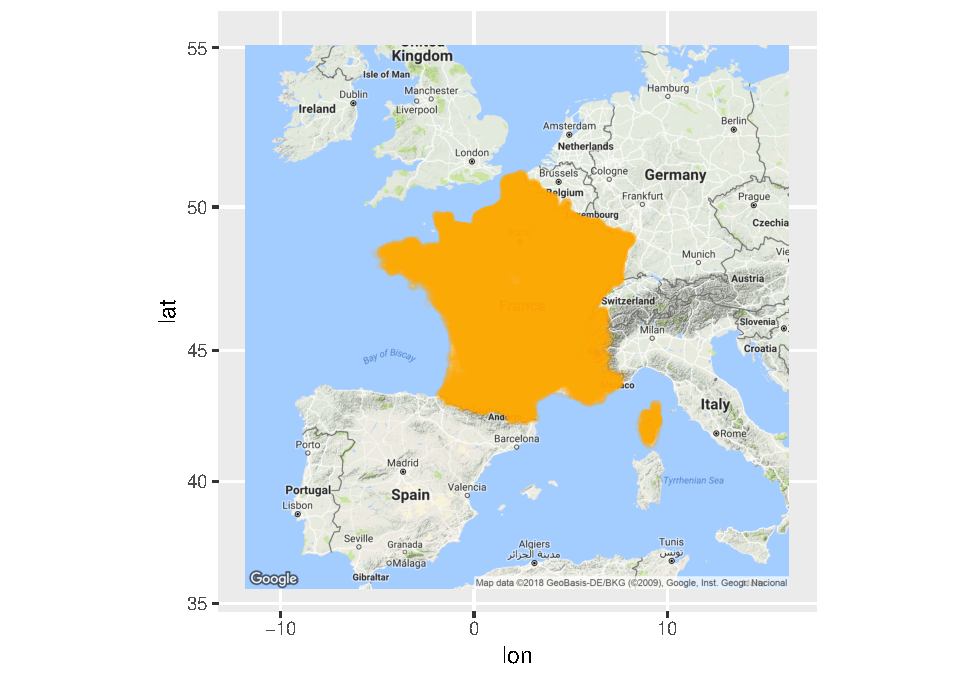
\includegraphics{TSLproject_files/figure-latex/unnamed-chunk-11-3.pdf}

\subsection{What we have learned}\label{what-we-have-learned-1}

Solved:

\begin{itemize}
\tightlist
\item
  Why latitude is missing and not longitude?
\item
  There are some duplications.
\end{itemize}

To do:

\begin{itemize}
\tightlist
\item
  What to do with non-European towns?
\end{itemize}

\subsection{How to use these data}\label{how-to-use-these-data-1}

\begin{itemize}
\tightlist
\item
  Compare European towns vs.~old colonies?
\item
  Useful for all datasets/analyses
\end{itemize}

\section{Analyze salary data}\label{analyze-salary-data}

\subsection{Pre-processing}\label{pre-processing-2}

\begin{Shaded}
\begin{Highlighting}[]
\CommentTok{# preliminary checks}
\KeywordTok{dim}\NormalTok{(salary)}
\end{Highlighting}
\end{Shaded}

\begin{verbatim}
## [1] 5136   26
\end{verbatim}

\begin{Shaded}
\begin{Highlighting}[]
\KeywordTok{names}\NormalTok{(salary)}
\end{Highlighting}
\end{Shaded}

\begin{verbatim}
##  [1] "CODGEO"           "town"             "sal_general"     
##  [4] "sal_executive"    "sal_midManager"   "sal_employee"    
##  [7] "sal_worker"       "sal_Females"      "sal_F_executive" 
## [10] "sal_F_midManager" "sal_F_employee"   "sal_F_worker"    
## [13] "sal_Males"        "sal_M_executive"  "sal_M_midManager"
## [16] "sal_M_employee"   "sal_M_worker"     "sal_18_25"       
## [19] "sal_26_50"        "sal_51plus"       "sal_F_18_25"     
## [22] "sal_F_26_50"      "sal_F_51plus"     "sal_M_18_25"     
## [25] "sal_M_26_50"      "sal_M_51plus"
\end{verbatim}

\begin{Shaded}
\begin{Highlighting}[]
\KeywordTok{head}\NormalTok{(salary)}
\end{Highlighting}
\end{Shaded}

\begin{verbatim}
##   CODGEO              town sal_general sal_executive sal_midManager
## 1  01004 Ambérieu-en-Bugey        13.7          24.2           15.5
## 2  01007          Ambronay        13.5          22.1           14.7
## 3  01014            Arbent        13.5          27.6           15.6
## 4  01024          Attignat        12.9          21.8           14.1
## 5  01025     Bâgé-la-Ville        13.0          22.8           14.1
## 6  01027             Balan        13.9          22.2           15.1
##   sal_employee sal_worker sal_Females sal_F_executive sal_F_midManager
## 1         10.3       11.2        11.6            19.1             13.2
## 2         10.7       11.4        11.9            19.0             13.3
## 3         11.1       11.1        10.9            19.5             11.7
## 4         11.0       11.3        11.4            19.0             13.0
## 5         10.5       11.1        11.6            19.4             13.6
## 6         11.0       11.4        12.5            20.3             14.0
##   sal_F_employee sal_F_worker sal_Males sal_M_executive sal_M_midManager
## 1           10.1          9.6      15.0            26.4             16.7
## 2           10.6         10.0      14.7            23.3             15.8
## 3           10.8          9.5      15.3            30.2             17.2
## 4           10.3          9.9      13.8            23.0             14.7
## 5           10.2          9.8      13.8            24.1             14.4
## 6           10.9         10.5      15.2            23.1             15.9
##   sal_M_employee sal_M_worker sal_18_25 sal_26_50 sal_51plus sal_F_18_25
## 1           11.0         11.6      10.5      13.7       16.1         9.7
## 2           11.3         11.7       9.8      13.8       14.6         9.2
## 3           12.4         11.8       9.3      13.3       16.0         8.9
## 4           13.2         11.6       9.6      12.9       14.2         9.3
## 5           11.7         11.4       9.4      12.8       15.2         9.0
## 6           12.1         11.7       9.7      14.1       15.4         9.5
##   sal_F_26_50 sal_F_51plus sal_M_18_25 sal_M_26_50 sal_M_51plus
## 1        11.8         12.5        11.0        14.9         18.6
## 2        12.2         12.5        10.2        14.9         16.4
## 3        10.6         12.5         9.6        15.1         18.6
## 4        11.4         12.2         9.7        13.8         15.9
## 5        11.8         12.3         9.7        13.4         16.9
## 6        12.8         13.0         9.9        15.3         17.2
\end{verbatim}

\begin{Shaded}
\begin{Highlighting}[]
\KeywordTok{str}\NormalTok{(salary)}
\end{Highlighting}
\end{Shaded}

\begin{verbatim}
## 'data.frame':    5136 obs. of  26 variables:
##  $ CODGEO          : chr  "01004" "01007" "01014" "01024" ...
##  $ town            : Factor w/ 5085 levels "Abbeville","Ablis",..: 73 79 133 192 275 298 407 395 400 406 ...
##  $ sal_general     : num  13.7 13.5 13.5 12.9 13 13.9 12.4 14 11.5 12.4 ...
##  $ sal_executive   : num  24.2 22.1 27.6 21.8 22.8 22.2 24 23.1 21.2 23.4 ...
##  $ sal_midManager  : num  15.5 14.7 15.6 14.1 14.1 15.1 13.1 15.3 13.5 14.1 ...
##  $ sal_employee    : num  10.3 10.7 11.1 11 10.5 11 10.5 10.9 9.9 10.3 ...
##  $ sal_worker      : num  11.2 11.4 11.1 11.3 11.1 11.4 10.4 11.3 10.5 10.5 ...
##  $ sal_Females     : num  11.6 11.9 10.9 11.4 11.6 12.5 10.9 12.4 10.3 11 ...
##  $ sal_F_executive : num  19.1 19 19.5 19 19.4 20.3 20.7 20.5 20.8 21.5 ...
##  $ sal_F_midManager: num  13.2 13.3 11.7 13 13.6 14 11.8 13.9 12.3 13 ...
##  $ sal_F_employee  : num  10.1 10.6 10.8 10.3 10.2 10.9 10.4 10.7 9.8 9.9 ...
##  $ sal_F_worker    : num  9.6 10 9.5 9.9 9.8 10.5 9.3 10.3 9 9.5 ...
##  $ sal_Males       : num  15 14.7 15.3 13.8 13.8 15.2 13.4 15.4 12.3 13.2 ...
##  $ sal_M_executive : num  26.4 23.3 30.2 23 24.1 23.1 25.2 24.4 21.3 24 ...
##  $ sal_M_midManager: num  16.7 15.8 17.2 14.7 14.4 15.9 13.8 16.3 14.2 14.9 ...
##  $ sal_M_employee  : num  11 11.3 12.4 13.2 11.7 12.1 10.8 11.8 10.5 11.6 ...
##  $ sal_M_worker    : num  11.6 11.7 11.8 11.6 11.4 11.7 10.8 11.6 11 10.9 ...
##  $ sal_18_25       : num  10.5 9.8 9.3 9.6 9.4 9.7 9.3 9.7 9.6 9.7 ...
##  $ sal_26_50       : num  13.7 13.8 13.3 12.9 12.8 14.1 12.5 13.9 11.5 12.3 ...
##  $ sal_51plus      : num  16.1 14.6 16 14.2 15.2 15.4 13.3 16.7 12.7 13.7 ...
##  $ sal_F_18_25     : num  9.7 9.2 8.9 9.3 9 9.5 8.9 9.7 9.2 9.3 ...
##  $ sal_F_26_50     : num  11.8 12.2 10.6 11.4 11.8 12.8 11 12.4 10.3 11.2 ...
##  $ sal_F_51plus    : num  12.5 12.5 12.5 12.2 12.3 13 11.5 13.8 11.3 11.4 ...
##  $ sal_M_18_25     : num  11 10.2 9.6 9.7 9.7 9.9 9.6 9.6 10 9.9 ...
##  $ sal_M_26_50     : num  14.9 14.9 15.1 13.8 13.4 15.3 13.3 15 12.3 13 ...
##  $ sal_M_51plus    : num  18.6 16.4 18.6 15.9 16.9 17.2 14.9 19.3 13.9 15.4 ...
\end{verbatim}

\begin{Shaded}
\begin{Highlighting}[]
\KeywordTok{summary}\NormalTok{(salary)}
\end{Highlighting}
\end{Shaded}

\begin{verbatim}
##     CODGEO                    town       sal_general    sal_executive 
##  Length:5136        Sainte-Marie:   4   Min.   :10.20   Min.   :16.0  
##  Class :character   Saint-Ouen  :   3   1st Qu.:12.10   1st Qu.:21.9  
##  Mode  :character   Allonnes    :   2   Median :13.00   Median :23.2  
##                     Andilly     :   2   Mean   :13.71   Mean   :23.7  
##                     Bassens     :   2   3rd Qu.:14.40   3rd Qu.:24.9  
##                     Beaumont    :   2   Max.   :43.30   Max.   :51.5  
##                     (Other)     :5121                                 
##  sal_midManager   sal_employee     sal_worker     sal_Females   
##  Min.   :11.60   Min.   : 8.70   Min.   : 8.30   Min.   : 9.30  
##  1st Qu.:13.80   1st Qu.:10.00   1st Qu.:10.60   1st Qu.:10.90  
##  Median :14.40   Median :10.40   Median :11.00   Median :11.50  
##  Mean   :14.58   Mean   :10.56   Mean   :11.24   Mean   :12.04  
##  3rd Qu.:15.10   3rd Qu.:10.90   3rd Qu.:11.60   3rd Qu.:12.70  
##  Max.   :54.60   Max.   :17.50   Max.   :46.30   Max.   :26.70  
##                                                                 
##  sal_F_executive sal_F_midManager sal_F_employee   sal_F_worker   
##  Min.   :12.00   Min.   :10.60    Min.   : 8.70   Min.   : 6.100  
##  1st Qu.:18.80   1st Qu.:12.60    1st Qu.: 9.80   1st Qu.: 9.200  
##  Median :20.00   Median :13.10    Median :10.10   Median : 9.700  
##  Mean   :20.22   Mean   :13.27    Mean   :10.31   Mean   : 9.827  
##  3rd Qu.:21.40   3rd Qu.:13.80    3rd Qu.:10.60   3rd Qu.:10.200  
##  Max.   :35.50   Max.   :19.00    Max.   :16.10   Max.   :28.100  
##                                                                   
##    sal_Males     sal_M_executive sal_M_midManager sal_M_employee 
##  Min.   :10.40   Min.   :13.8    Min.   :11.80    Min.   : 8.00  
##  1st Qu.:12.90   1st Qu.:23.1    1st Qu.:14.50    1st Qu.:10.50  
##  Median :14.10   Median :24.6    Median :15.20    Median :11.10  
##  Mean   :14.85   Mean   :25.2    Mean   :15.49    Mean   :11.27  
##  3rd Qu.:15.80   3rd Qu.:26.6    3rd Qu.:16.00    3rd Qu.:11.80  
##  Max.   :52.40   Max.   :58.0    Max.   :93.40    Max.   :23.50  
##                                                                  
##   sal_M_worker    sal_18_25       sal_26_50      sal_51plus   
##  Min.   : 8.9   Min.   : 7.90   Min.   : 9.7   Min.   :10.50  
##  1st Qu.:10.8   1st Qu.: 9.20   1st Qu.:12.0   1st Qu.:13.70  
##  Median :11.3   Median : 9.50   Median :12.9   Median :15.00  
##  Mean   :11.5   Mean   : 9.55   Mean   :13.5   Mean   :15.88  
##  3rd Qu.:11.9   3rd Qu.: 9.70   3rd Qu.:14.3   3rd Qu.:16.90  
##  Max.   :53.2   Max.   :60.60   Max.   :38.1   Max.   :56.90  
##                                                               
##   sal_F_18_25      sal_F_26_50     sal_F_51plus    sal_M_18_25    
##  Min.   : 7.500   Min.   : 9.10   Min.   : 9.50   Min.   : 7.800  
##  1st Qu.: 8.900   1st Qu.:10.90   1st Qu.:11.70   1st Qu.: 9.400  
##  Median : 9.100   Median :11.60   Median :12.60   Median : 9.700  
##  Mean   : 9.162   Mean   :12.06   Mean   :13.17   Mean   : 9.821  
##  3rd Qu.: 9.400   3rd Qu.:12.70   3rd Qu.:14.00   3rd Qu.:10.000  
##  Max.   :12.000   Max.   :26.60   Max.   :31.00   Max.   :93.300  
##                                                                   
##   sal_M_26_50     sal_M_51plus  
##  Min.   : 9.60   Min.   :10.80  
##  1st Qu.:12.70   1st Qu.:14.90  
##  Median :13.80   Median :16.60  
##  Mean   :14.49   Mean   :17.68  
##  3rd Qu.:15.50   3rd Qu.:19.00  
##  Max.   :45.40   Max.   :68.60  
## 
\end{verbatim}

\begin{Shaded}
\begin{Highlighting}[]
\CommentTok{# Drop unnecessary columns (town name repeats in other table, is it surely possible to merge them?)}
\KeywordTok{names}\NormalTok{(salary)}
\end{Highlighting}
\end{Shaded}

\begin{verbatim}
##  [1] "CODGEO"           "town"             "sal_general"     
##  [4] "sal_executive"    "sal_midManager"   "sal_employee"    
##  [7] "sal_worker"       "sal_Females"      "sal_F_executive" 
## [10] "sal_F_midManager" "sal_F_employee"   "sal_F_worker"    
## [13] "sal_Males"        "sal_M_executive"  "sal_M_midManager"
## [16] "sal_M_employee"   "sal_M_worker"     "sal_18_25"       
## [19] "sal_26_50"        "sal_51plus"       "sal_F_18_25"     
## [22] "sal_F_26_50"      "sal_F_51plus"     "sal_M_18_25"     
## [25] "sal_M_26_50"      "sal_M_51plus"
\end{verbatim}

\begin{Shaded}
\begin{Highlighting}[]
\CommentTok{# salary <- subset(salary, select = -c(town))}

\CommentTok{# Convert CODGEO to numeric}
\NormalTok{salary}\OperatorTok{$}\NormalTok{CODGEO <-}\StringTok{ }\KeywordTok{as.numeric}\NormalTok{(}\KeywordTok{as.character}\NormalTok{(salary}\OperatorTok{$}\NormalTok{CODGEO))}

\CommentTok{# Check for duplicated data}
\KeywordTok{sum}\NormalTok{(}\KeywordTok{duplicated.data.frame}\NormalTok{(salary))}
\end{Highlighting}
\end{Shaded}

\begin{verbatim}
## [1] 0
\end{verbatim}

\subsection{EDA}\label{eda-2}

Univariate analysis comparing various job categories for both genders:

\begin{Shaded}
\begin{Highlighting}[]
\KeywordTok{require}\NormalTok{(ggplot2)}

\CommentTok{#  number of units}
\NormalTok{n_sex <-}\StringTok{ }\KeywordTok{length}\NormalTok{(salary}\OperatorTok{$}\NormalTok{sal_Females)}

\CommentTok{# vector representing males and females}
\NormalTok{Label <-}\StringTok{ }\KeywordTok{c}\NormalTok{(}\KeywordTok{rep}\NormalTok{(}\StringTok{"M"}\NormalTok{, n_sex}\OperatorTok{*}\DecValTok{5}\NormalTok{), }\KeywordTok{rep}\NormalTok{(}\StringTok{"F"}\NormalTok{, n_sex}\OperatorTok{*}\DecValTok{5}\NormalTok{))}

\CommentTok{# vector representing the variable considered}
\NormalTok{Variable <-}\StringTok{ }\KeywordTok{c}\NormalTok{(}\KeywordTok{rep}\NormalTok{(}\StringTok{"General"}\NormalTok{, n_sex), }
             \KeywordTok{rep}\NormalTok{(}\StringTok{"Executive"}\NormalTok{, n_sex),}
             \KeywordTok{rep}\NormalTok{(}\StringTok{"MidManager"}\NormalTok{, n_sex),}
             \KeywordTok{rep}\NormalTok{(}\StringTok{"Employee"}\NormalTok{, n_sex),}
             \KeywordTok{rep}\NormalTok{(}\StringTok{"Worker"}\NormalTok{,n_sex),}
             \KeywordTok{rep}\NormalTok{(}\StringTok{"General"}\NormalTok{, n_sex), }
             \KeywordTok{rep}\NormalTok{(}\StringTok{"Executive"}\NormalTok{, n_sex),}
             \KeywordTok{rep}\NormalTok{(}\StringTok{"MidManager"}\NormalTok{, n_sex),}
             \KeywordTok{rep}\NormalTok{(}\StringTok{"Employee"}\NormalTok{, n_sex),}
             \KeywordTok{rep}\NormalTok{(}\StringTok{"Worker"}\NormalTok{,n_sex))}

\CommentTok{# merge these data}
\NormalTok{sal_sex =}\StringTok{ }\KeywordTok{cbind.data.frame}\NormalTok{(}\DataTypeTok{Label =}\NormalTok{ Label, }
             \DataTypeTok{value =} \KeywordTok{c}\NormalTok{(salary}\OperatorTok{$}\NormalTok{sal_Males, salary}\OperatorTok{$}\NormalTok{sal_M_executive, salary}\OperatorTok{$}\NormalTok{sal_M_midManager, salary}\OperatorTok{$}\NormalTok{sal_M_employee, salary}\OperatorTok{$}\NormalTok{sal_M_worker,}
\NormalTok{                       salary}\OperatorTok{$}\NormalTok{sal_Females, salary}\OperatorTok{$}\NormalTok{sal_F_executive, salary}\OperatorTok{$}\NormalTok{sal_F_midManager, salary}\OperatorTok{$}\NormalTok{sal_F_employee, salary}\OperatorTok{$}\NormalTok{sal_F_worker),}
             \DataTypeTok{Variable =}\NormalTok{ Variable)}

\CommentTok{# plotting phase}
\NormalTok{p <-}\StringTok{  }\KeywordTok{ggplot}\NormalTok{(}\DataTypeTok{data =}\NormalTok{ sal_sex, }\KeywordTok{aes}\NormalTok{(}\DataTypeTok{x=}\NormalTok{Label, }\DataTypeTok{y=}\NormalTok{value)) }\OperatorTok{+}
\StringTok{      }\KeywordTok{geom_boxplot}\NormalTok{(}\KeywordTok{aes}\NormalTok{(}\DataTypeTok{fill =}\NormalTok{ Label)) }\OperatorTok{+}
\StringTok{      }\CommentTok{# not color points replacing colour = group instead of colour=Label}
\StringTok{      }\KeywordTok{geom_point}\NormalTok{(}\KeywordTok{aes}\NormalTok{(}\DataTypeTok{y=}\NormalTok{value, }\DataTypeTok{colour=}\NormalTok{Label), }\DataTypeTok{position =} \KeywordTok{position_dodge}\NormalTok{(}\DataTypeTok{width=}\FloatTok{0.75}\NormalTok{)) }\OperatorTok{+}
\StringTok{      }\KeywordTok{facet_wrap}\NormalTok{( }\OperatorTok{~}\StringTok{ }\NormalTok{Variable, }\DataTypeTok{scales=}\StringTok{"free"}\NormalTok{) }\OperatorTok{+}
\StringTok{      }\KeywordTok{xlab}\NormalTok{(}\StringTok{"x-axis"}\NormalTok{) }\OperatorTok{+}\StringTok{ }\KeywordTok{ylab}\NormalTok{(}\StringTok{"y-axis"}\NormalTok{) }\OperatorTok{+}\StringTok{ }\KeywordTok{ggtitle}\NormalTok{(}\StringTok{"Gender comparison"}\NormalTok{) }\OperatorTok{+}
\StringTok{      }\KeywordTok{stat_boxplot}\NormalTok{(}\DataTypeTok{geom =} \StringTok{"errorbar"}\NormalTok{, }\DataTypeTok{width =} \FloatTok{0.5}\NormalTok{)}
      \CommentTok{# p <- p + guides(fill=guide_legend(title="Legend"))}
\NormalTok{p}
\end{Highlighting}
\end{Shaded}

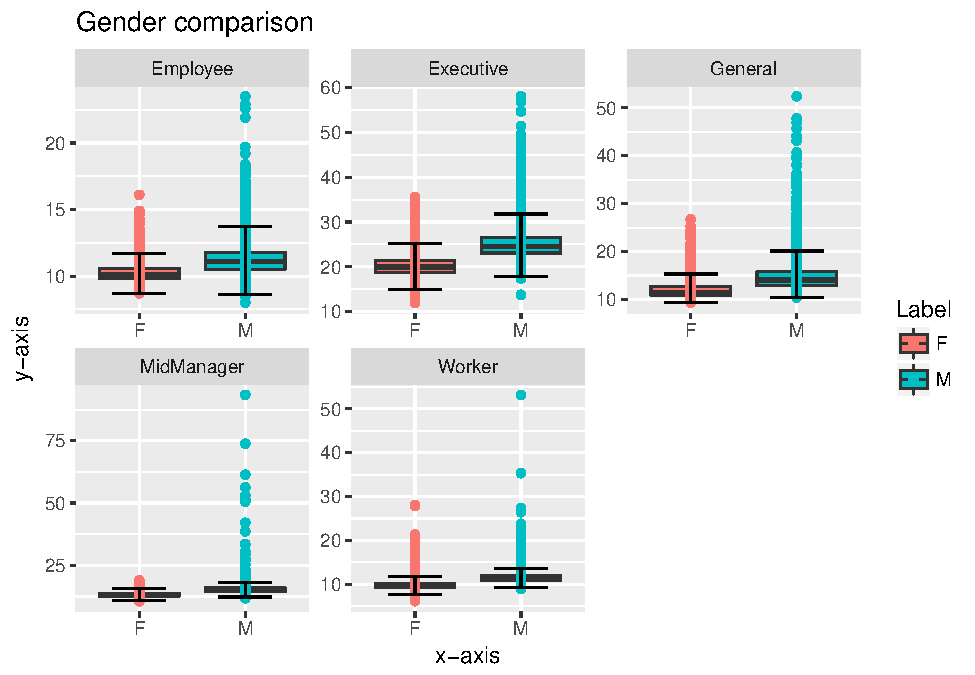
\includegraphics{TSLproject_files/figure-latex/unnamed-chunk-13-1.pdf}

\begin{Shaded}
\begin{Highlighting}[]
\CommentTok{# excluding outliers}
\NormalTok{p2 <-}\StringTok{ }\KeywordTok{ggplot}\NormalTok{(}\DataTypeTok{data =}\NormalTok{ sal_sex, }\KeywordTok{aes}\NormalTok{(}\DataTypeTok{x=}\NormalTok{Label, }\DataTypeTok{y=}\NormalTok{value)) }\OperatorTok{+}
\StringTok{      }\KeywordTok{scale_y_continuous}\NormalTok{(}\DataTypeTok{limits =} \KeywordTok{quantile}\NormalTok{(sal_sex}\OperatorTok{$}\NormalTok{value, }\KeywordTok{c}\NormalTok{(}\DecValTok{0}\NormalTok{, }\FloatTok{0.9}\NormalTok{))) }\OperatorTok{+}
\StringTok{      }\KeywordTok{geom_boxplot}\NormalTok{(}\KeywordTok{aes}\NormalTok{(}\DataTypeTok{fill =}\NormalTok{ Label)) }\OperatorTok{+}
\StringTok{      }\CommentTok{# not color points replacing colour = group instead of colour=Label}
\StringTok{      }\KeywordTok{geom_point}\NormalTok{(}\KeywordTok{aes}\NormalTok{(}\DataTypeTok{y=}\NormalTok{value, }\DataTypeTok{colour=}\NormalTok{Label), }\DataTypeTok{position =} \KeywordTok{position_dodge}\NormalTok{(}\DataTypeTok{width=}\FloatTok{0.75}\NormalTok{)) }\OperatorTok{+}
\StringTok{      }\KeywordTok{facet_wrap}\NormalTok{( }\OperatorTok{~}\StringTok{ }\NormalTok{Variable, }\DataTypeTok{scales=}\StringTok{"free"}\NormalTok{) }\OperatorTok{+}
\StringTok{      }\KeywordTok{xlab}\NormalTok{(}\StringTok{"x-axis"}\NormalTok{) }\OperatorTok{+}\StringTok{ }\KeywordTok{ylab}\NormalTok{(}\StringTok{"y-axis"}\NormalTok{) }\OperatorTok{+}\StringTok{ }\KeywordTok{ggtitle}\NormalTok{(}\StringTok{"Gender comparison excluding the last decile"}\NormalTok{) }\OperatorTok{+}
\StringTok{      }\CommentTok{# p <- p + guides(fill=guide_legend(title="Legend"))}
\StringTok{      }\KeywordTok{stat_boxplot}\NormalTok{(}\DataTypeTok{geom =} \StringTok{"errorbar"}\NormalTok{, }\DataTypeTok{width =} \FloatTok{0.5}\NormalTok{)}
\NormalTok{p2}
\end{Highlighting}
\end{Shaded}

\begin{verbatim}
## Warning: Removed 5067 rows containing non-finite values (stat_boxplot).

## Warning: Removed 5067 rows containing non-finite values (stat_boxplot).
\end{verbatim}

\begin{verbatim}
## Warning: Removed 5067 rows containing missing values (geom_point).
\end{verbatim}

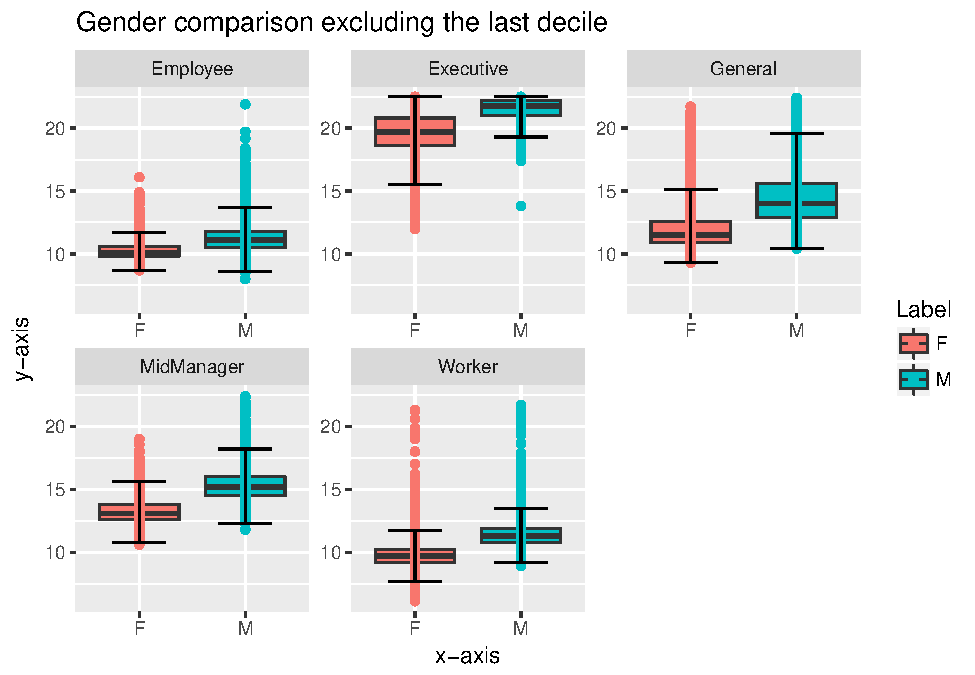
\includegraphics{TSLproject_files/figure-latex/unnamed-chunk-13-2.pdf}

Highlight bivariate relations using scatter matrices:

\begin{Shaded}
\begin{Highlighting}[]
\CommentTok{# most general pairs}
\KeywordTok{pairs}\NormalTok{(salary[}\KeywordTok{c}\NormalTok{(}\DecValTok{3}\OperatorTok{:}\DecValTok{8}\NormalTok{, }\DecValTok{13}\NormalTok{, }\DecValTok{18}\OperatorTok{:}\DecValTok{20}\NormalTok{)])}
\end{Highlighting}
\end{Shaded}

\includegraphics{TSLproject_files/figure-latex/unnamed-chunk-14-1.pdf}

\begin{Shaded}
\begin{Highlighting}[]
\CommentTok{# pairs highlighting genders' differences}
\KeywordTok{pairs}\NormalTok{(salary[}\KeywordTok{c}\NormalTok{(}\DecValTok{9}\OperatorTok{:}\DecValTok{12}\NormalTok{, }\DecValTok{14}\OperatorTok{:}\DecValTok{17}\NormalTok{)])}
\end{Highlighting}
\end{Shaded}

\includegraphics{TSLproject_files/figure-latex/unnamed-chunk-14-2.pdf}

Fit a regression model to predict the salaries of people in age 26-50
using as regressor 51+ years:

\begin{Shaded}
\begin{Highlighting}[]
\CommentTok{# fit and show OLS estimate}
\KeywordTok{plot}\NormalTok{(salary}\OperatorTok{$}\NormalTok{sal_26_}\DecValTok{50} \OperatorTok{~}\StringTok{ }\NormalTok{salary}\OperatorTok{$}\NormalTok{sal_51plus)}
\end{Highlighting}
\end{Shaded}

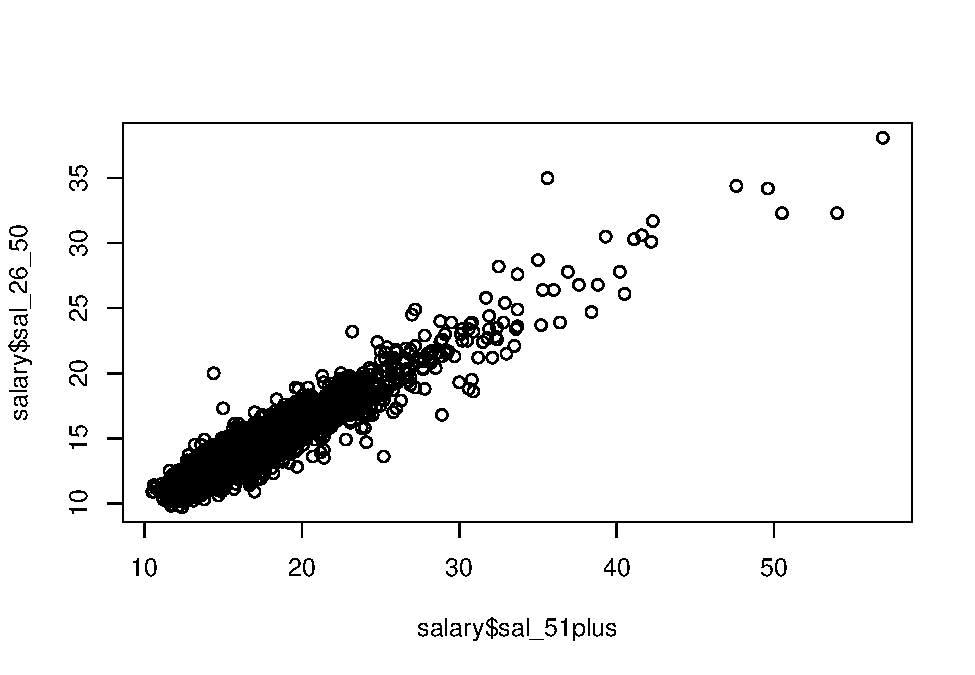
\includegraphics{TSLproject_files/figure-latex/unnamed-chunk-15-1.pdf}

\begin{Shaded}
\begin{Highlighting}[]
\NormalTok{fit_LM_26_}\DecValTok{50}\NormalTok{ =}\StringTok{ }\KeywordTok{glm}\NormalTok{(salary}\OperatorTok{$}\NormalTok{sal_26_}\DecValTok{50} \OperatorTok{~}\StringTok{ }\NormalTok{salary}\OperatorTok{$}\NormalTok{sal_51plus, }\DataTypeTok{data =}\NormalTok{ salary)}
\KeywordTok{abline}\NormalTok{(fit_LM_26_}\DecValTok{50}\NormalTok{, }\DataTypeTok{lwd=}\DecValTok{3}\NormalTok{, }\DataTypeTok{col=}\StringTok{"red"}\NormalTok{)}
\end{Highlighting}
\end{Shaded}

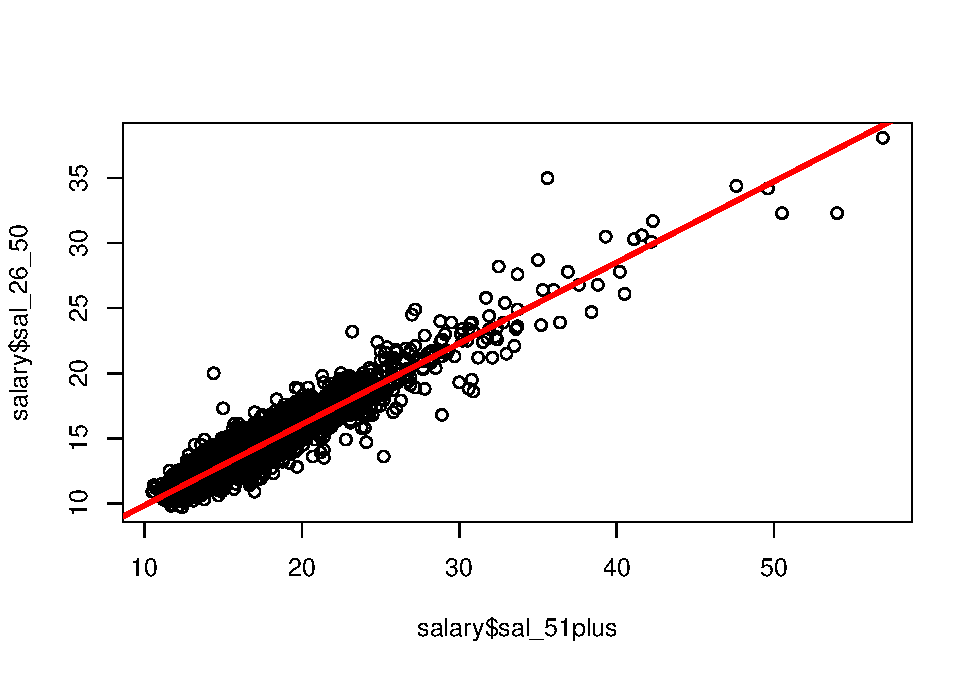
\includegraphics{TSLproject_files/figure-latex/unnamed-chunk-15-2.pdf}

\begin{Shaded}
\begin{Highlighting}[]
\CommentTok{# diagnostics}
\KeywordTok{summary}\NormalTok{(fit_LM_26_}\DecValTok{50}\NormalTok{)}
\end{Highlighting}
\end{Shaded}

\begin{verbatim}
## 
## Call:
## glm(formula = salary$sal_26_50 ~ salary$sal_51plus, data = salary)
## 
## Deviance Residuals: 
##     Min       1Q   Median       3Q      Max  
## -5.7024  -0.4395  -0.0228   0.4069   9.2197  
## 
## Coefficients:
##                   Estimate Std. Error t value Pr(>|t|)    
## (Intercept)       3.605893   0.048896   73.75   <2e-16 ***
## salary$sal_51plus 0.622877   0.003004  207.35   <2e-16 ***
## ---
## Signif. codes:  0 '***' 0.001 '**' 0.01 '*' 0.05 '.' 0.1 ' ' 1
## 
## (Dispersion parameter for gaussian family taken to be 0.595825)
## 
##     Null deviance: 28676  on 5135  degrees of freedom
## Residual deviance:  3059  on 5134  degrees of freedom
## AIC: 11920
## 
## Number of Fisher Scoring iterations: 2
\end{verbatim}

\begin{Shaded}
\begin{Highlighting}[]
\KeywordTok{plot}\NormalTok{(fit_LM_26_}\DecValTok{50}\NormalTok{)}
\end{Highlighting}
\end{Shaded}

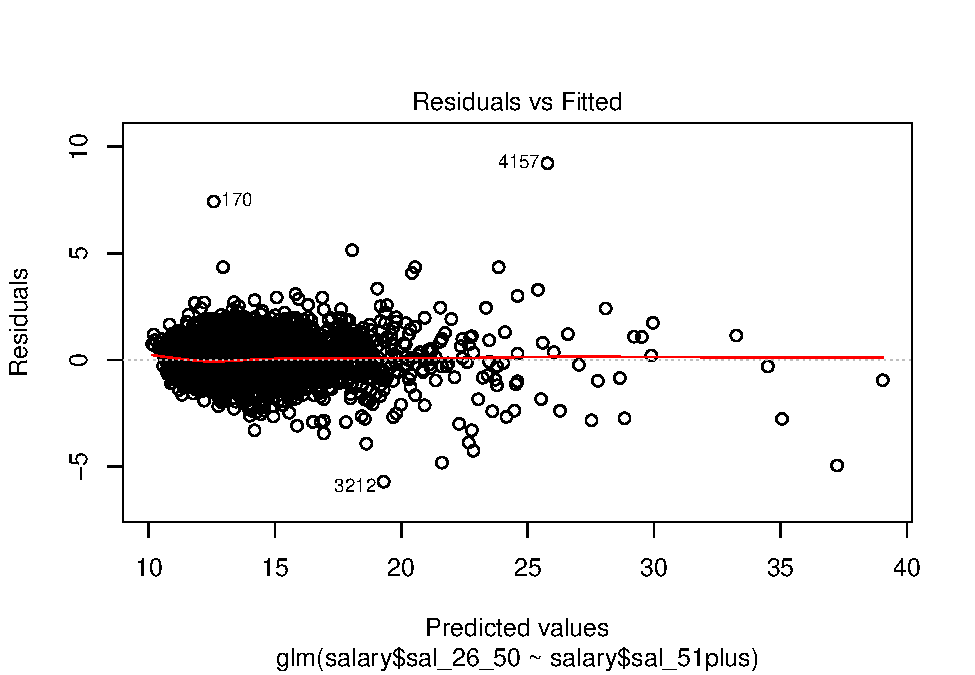
\includegraphics{TSLproject_files/figure-latex/unnamed-chunk-15-3.pdf}
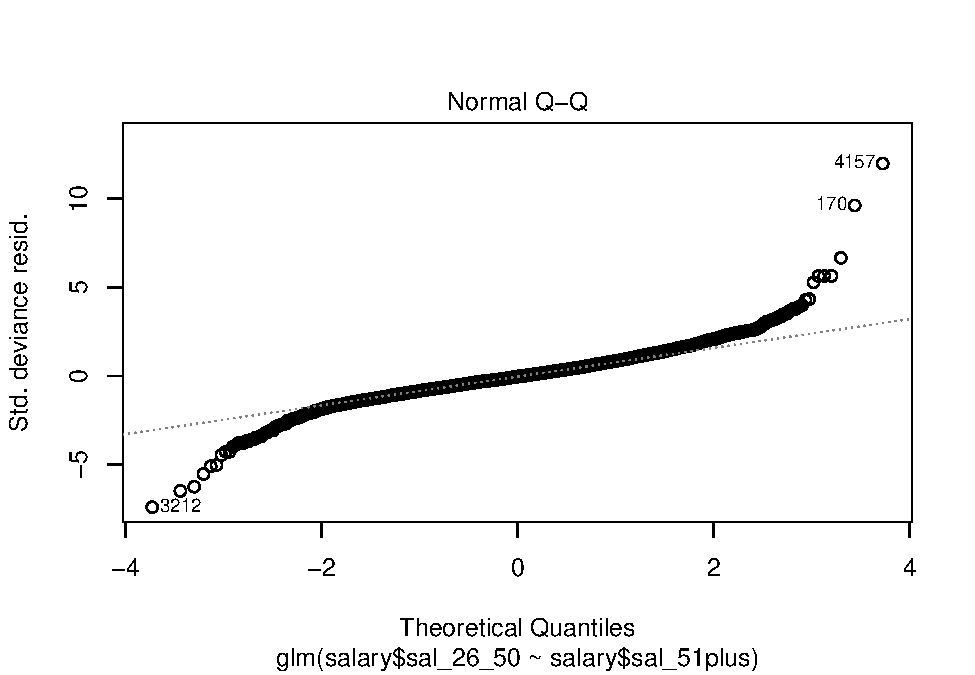
\includegraphics{TSLproject_files/figure-latex/unnamed-chunk-15-4.pdf}
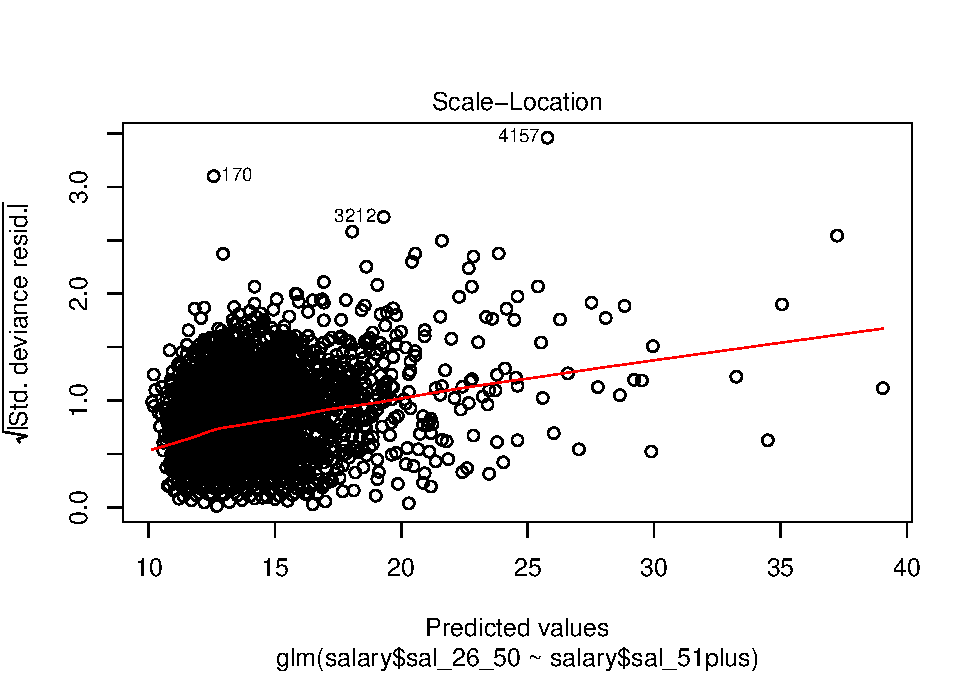
\includegraphics{TSLproject_files/figure-latex/unnamed-chunk-15-5.pdf}
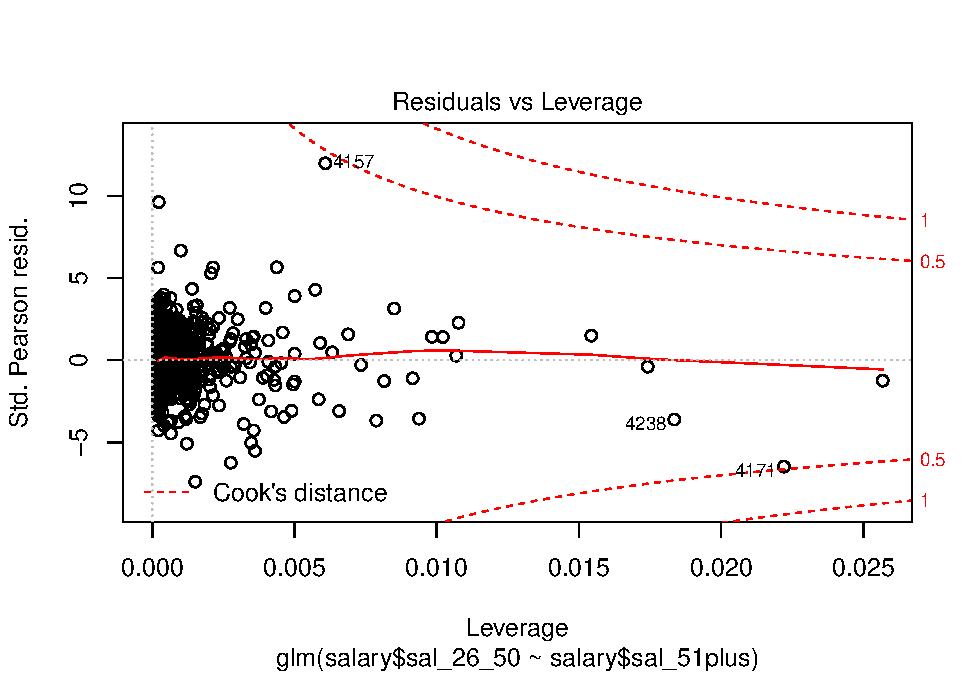
\includegraphics{TSLproject_files/figure-latex/unnamed-chunk-15-6.pdf}

Same as before but adding polynomials which are evauated using 10-folds
cross validation:

\begin{Shaded}
\begin{Highlighting}[]
\KeywordTok{require}\NormalTok{(boot)}
\end{Highlighting}
\end{Shaded}

\begin{verbatim}
## Loading required package: boot
\end{verbatim}

\begin{Shaded}
\begin{Highlighting}[]
\KeywordTok{set.seed}\NormalTok{(}\DecValTok{1}\NormalTok{)}

\CommentTok{# k-Fold Cross-Validation}
\NormalTok{cv.err.K =}\StringTok{ }\KeywordTok{rep}\NormalTok{(}\DecValTok{0}\NormalTok{, }\DecValTok{5}\NormalTok{)}
\NormalTok{cv.err.K =}\StringTok{ }\KeywordTok{rbind}\NormalTok{(cv.err.K, cv.err.K)}
\ControlFlowTok{for}\NormalTok{ (i }\ControlFlowTok{in} \DecValTok{1}\OperatorTok{:}\DecValTok{5}\NormalTok{)\{}
\NormalTok{  fit_LM_26_}\FloatTok{50.}\NormalTok{K =}\StringTok{ }\KeywordTok{glm}\NormalTok{(sal_26_}\DecValTok{50} \OperatorTok{~}\StringTok{ }\KeywordTok{poly}\NormalTok{(sal_51plus, i), }\DataTypeTok{data =}\NormalTok{ salary)}
\NormalTok{  cv.err.K[,i] =}\StringTok{ }\KeywordTok{cv.glm}\NormalTok{(salary, fit_LM_26_}\FloatTok{50.}\NormalTok{K, }\DataTypeTok{K =} \DecValTok{10}\NormalTok{)}\OperatorTok{$}\NormalTok{delta[}\DecValTok{1}\NormalTok{]}
\NormalTok{\}}

\CommentTok{# plotting results}
\KeywordTok{plot}\NormalTok{(cv.err.K[}\DecValTok{1}\NormalTok{,], }\DataTypeTok{type =} \StringTok{'l'}\NormalTok{, }\DataTypeTok{col =} \StringTok{'red'}\NormalTok{, }\DataTypeTok{xlab =} \StringTok{"Polynomials' order"}\NormalTok{, }
     \DataTypeTok{ylab =} \StringTok{"10-folds CV"}\NormalTok{, }\DataTypeTok{main =} \StringTok{"CV and adjusted CV for different polynomials"}\NormalTok{)}
\end{Highlighting}
\end{Shaded}

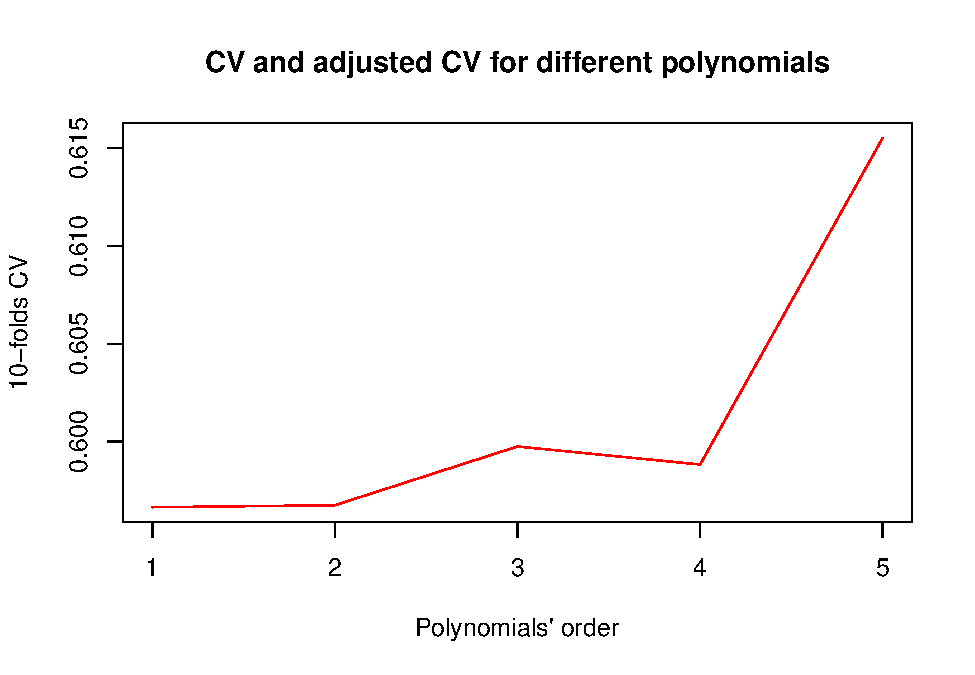
\includegraphics{TSLproject_files/figure-latex/unnamed-chunk-16-1.pdf}

\begin{Shaded}
\begin{Highlighting}[]
\KeywordTok{lines}\NormalTok{(cv.err.K[}\DecValTok{2}\NormalTok{,], }\DataTypeTok{col =} \StringTok{'green'}\NormalTok{)}
\end{Highlighting}
\end{Shaded}

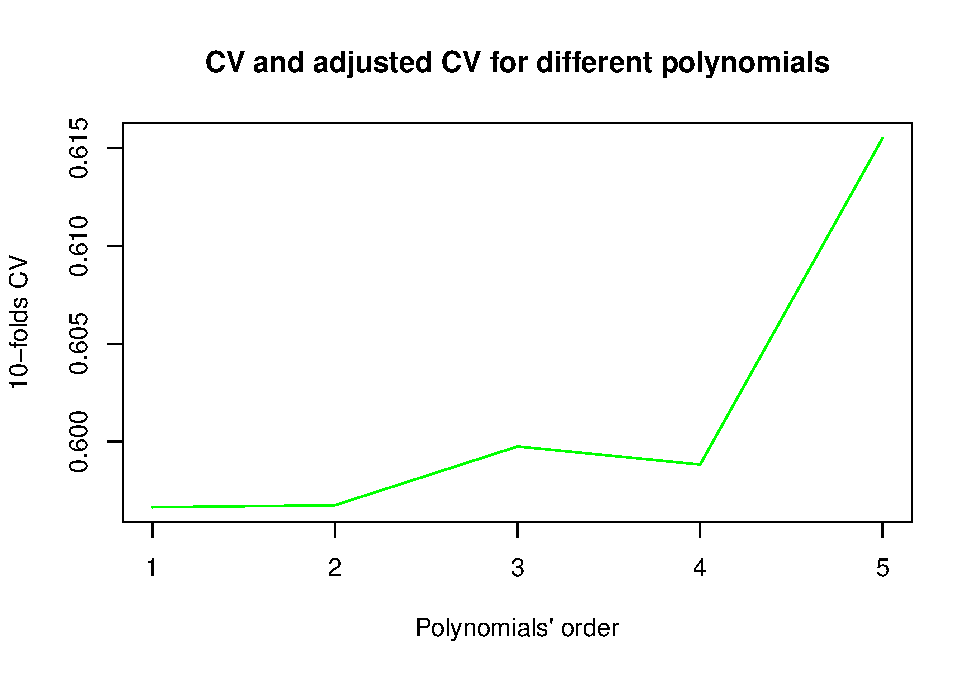
\includegraphics{TSLproject_files/figure-latex/unnamed-chunk-16-2.pdf}

\begin{Shaded}
\begin{Highlighting}[]
\KeywordTok{points}\NormalTok{(}\KeywordTok{which.min}\NormalTok{(cv.err.K), cv.err.K[}\DecValTok{1}\NormalTok{, }\KeywordTok{which.min}\NormalTok{(cv.err.K)], }\DataTypeTok{col =} \StringTok{"red"}\NormalTok{, }\DataTypeTok{cex=}\DecValTok{2}\NormalTok{, }\DataTypeTok{pch=}\DecValTok{20}\NormalTok{)}
\end{Highlighting}
\end{Shaded}

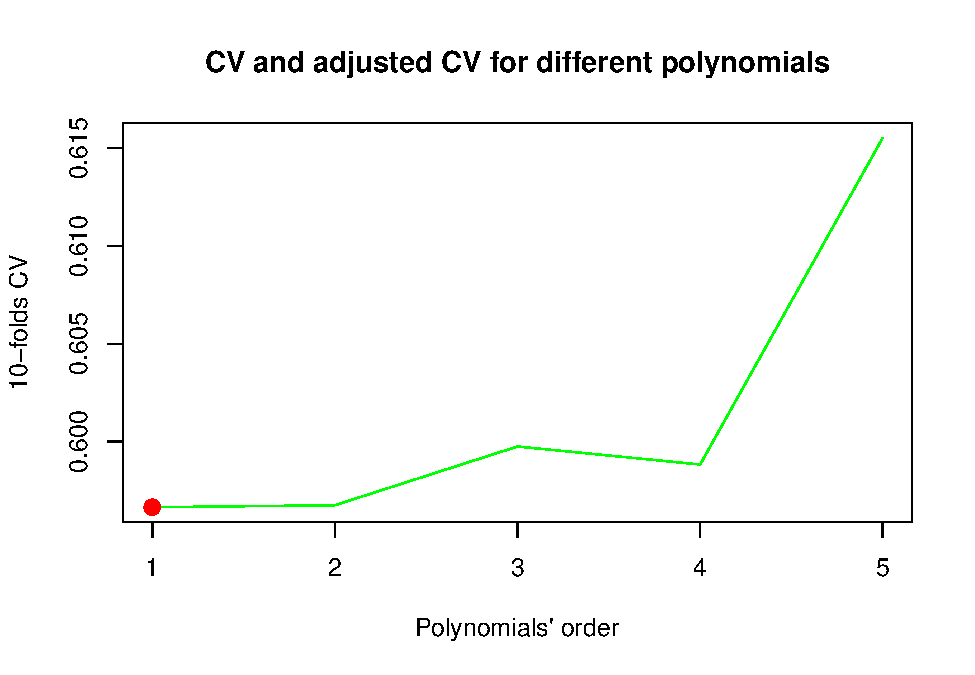
\includegraphics{TSLproject_files/figure-latex/unnamed-chunk-16-3.pdf}

\begin{Shaded}
\begin{Highlighting}[]
\KeywordTok{legend}\NormalTok{(}\StringTok{'topright'}\NormalTok{, }\DataTypeTok{legend =} \KeywordTok{c}\NormalTok{(}\StringTok{'CV'}\NormalTok{, }\StringTok{'Adj. CV'}\NormalTok{), }\DataTypeTok{col =} \KeywordTok{c}\NormalTok{(}\StringTok{'red'}\NormalTok{, }\StringTok{'green'}\NormalTok{), }\DataTypeTok{pch =} \DecValTok{10}\NormalTok{)}
\end{Highlighting}
\end{Shaded}

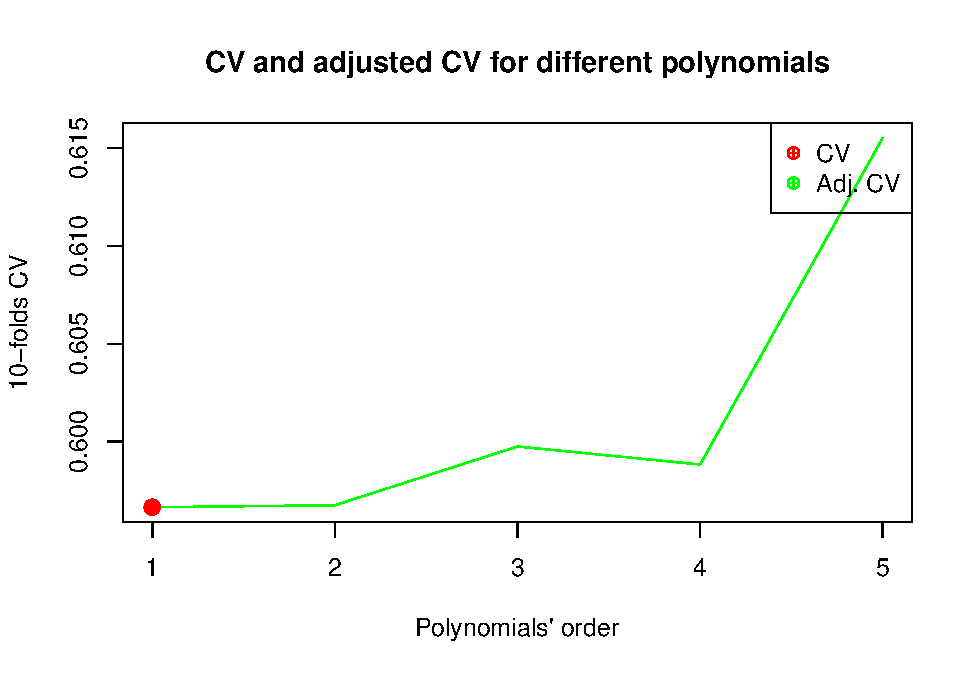
\includegraphics{TSLproject_files/figure-latex/unnamed-chunk-16-4.pdf}

Predicting sal\_executive with 5 regressers using Lasso with CV and
10-folds CV: {[} PROBLEM FOR COLLINEARITY? use ridge?{]} {[} add
polynomials? {]}

\begin{Shaded}
\begin{Highlighting}[]
\KeywordTok{require}\NormalTok{(glmnet)}
\end{Highlighting}
\end{Shaded}

\begin{verbatim}
## Loading required package: glmnet
\end{verbatim}

\begin{verbatim}
## Loading required package: Matrix
\end{verbatim}

\begin{verbatim}
## Loading required package: foreach
\end{verbatim}

\begin{verbatim}
## Loaded glmnet 2.0-13
\end{verbatim}

\begin{Shaded}
\begin{Highlighting}[]
\KeywordTok{set.seed}\NormalTok{(}\DecValTok{1}\NormalTok{)}

\CommentTok{# crate an X matrix excluding intercept}
\CommentTok{# x = cbind(salary$sal_midManager, salary$sal_employee, salary$sal_worker, salary$sal_18_25, salary$sal_51plus)}
\CommentTok{# y = salary$sal_executive}
\CommentTok{# probably for ridge}
\KeywordTok{names}\NormalTok{(salary)}
\end{Highlighting}
\end{Shaded}

\begin{verbatim}
##  [1] "CODGEO"           "town"             "sal_general"     
##  [4] "sal_executive"    "sal_midManager"   "sal_employee"    
##  [7] "sal_worker"       "sal_Females"      "sal_F_executive" 
## [10] "sal_F_midManager" "sal_F_employee"   "sal_F_worker"    
## [13] "sal_Males"        "sal_M_executive"  "sal_M_midManager"
## [16] "sal_M_employee"   "sal_M_worker"     "sal_18_25"       
## [19] "sal_26_50"        "sal_51plus"       "sal_F_18_25"     
## [22] "sal_F_26_50"      "sal_F_51plus"     "sal_M_18_25"     
## [25] "sal_M_26_50"      "sal_M_51plus"
\end{verbatim}

\begin{Shaded}
\begin{Highlighting}[]
\NormalTok{y =}\StringTok{ }\NormalTok{salary}\OperatorTok{$}\NormalTok{sal_26_}\DecValTok{50}
\NormalTok{x =}\StringTok{ }\KeywordTok{as.matrix}\NormalTok{(}\KeywordTok{cbind}\NormalTok{(salary[, }\KeywordTok{c}\NormalTok{(}\DecValTok{4}\OperatorTok{:}\DecValTok{8}\NormalTok{, }\DecValTok{13}\NormalTok{, }\DecValTok{18}\NormalTok{, }\DecValTok{20}\NormalTok{)]))}
\KeywordTok{names}\NormalTok{(x)}
\end{Highlighting}
\end{Shaded}

\begin{verbatim}
## NULL
\end{verbatim}

\begin{Shaded}
\begin{Highlighting}[]
\CommentTok{# grid for lambda values}
\NormalTok{grid =}\StringTok{ }\DecValTok{10}\OperatorTok{^}\KeywordTok{seq}\NormalTok{(}\DecValTok{1}\NormalTok{, }\OperatorTok{-}\DecValTok{5}\NormalTok{, }\DataTypeTok{length =} \DecValTok{100}\NormalTok{)}
\NormalTok{lasso.mod =}\StringTok{ }\KeywordTok{glmnet}\NormalTok{(x, y, }\DataTypeTok{alpha =} \DecValTok{1}\NormalTok{, }\DataTypeTok{lambda =}\NormalTok{ grid)}
\KeywordTok{dim}\NormalTok{(}\KeywordTok{coef}\NormalTok{(lasso.mod))}
\end{Highlighting}
\end{Shaded}

\begin{verbatim}
## [1]   9 100
\end{verbatim}

\begin{Shaded}
\begin{Highlighting}[]
\CommentTok{# the norms are increasing in value because of the shrinkage}
\NormalTok{lasso.mod}\OperatorTok{$}\NormalTok{lambda[}\DecValTok{1}\NormalTok{]                  }\CommentTok{# lambda value}
\end{Highlighting}
\end{Shaded}

\begin{verbatim}
## [1] 10
\end{verbatim}

\begin{Shaded}
\begin{Highlighting}[]
\KeywordTok{sqrt}\NormalTok{(}\KeywordTok{sum}\NormalTok{(}\KeywordTok{coef}\NormalTok{(lasso.mod)[}\OperatorTok{-}\DecValTok{1}\NormalTok{,}\DecValTok{1}\NormalTok{]}\OperatorTok{^}\DecValTok{2}\NormalTok{))   }\CommentTok{# L2 norm of its coeff}
\end{Highlighting}
\end{Shaded}

\begin{verbatim}
## [1] 0
\end{verbatim}

\begin{Shaded}
\begin{Highlighting}[]
\NormalTok{lasso.mod}\OperatorTok{$}\NormalTok{lambda[}\DecValTok{51}\NormalTok{]}
\end{Highlighting}
\end{Shaded}

\begin{verbatim}
## [1] 0.009326033
\end{verbatim}

\begin{Shaded}
\begin{Highlighting}[]
\KeywordTok{sqrt}\NormalTok{(}\KeywordTok{sum}\NormalTok{(}\KeywordTok{coef}\NormalTok{(lasso.mod)[}\OperatorTok{-}\DecValTok{1}\NormalTok{,}\DecValTok{51}\NormalTok{]}\OperatorTok{^}\DecValTok{2}\NormalTok{))}
\end{Highlighting}
\end{Shaded}

\begin{verbatim}
## [1] 0.8159349
\end{verbatim}

\begin{Shaded}
\begin{Highlighting}[]
\NormalTok{lasso.mod}\OperatorTok{$}\NormalTok{lambda[}\DecValTok{90}\NormalTok{]}
\end{Highlighting}
\end{Shaded}

\begin{verbatim}
## [1] 4.037017e-05
\end{verbatim}

\begin{Shaded}
\begin{Highlighting}[]
\KeywordTok{sqrt}\NormalTok{(}\KeywordTok{sum}\NormalTok{(}\KeywordTok{coef}\NormalTok{(lasso.mod)[}\OperatorTok{-}\DecValTok{1}\NormalTok{,}\DecValTok{90}\NormalTok{]}\OperatorTok{^}\DecValTok{2}\NormalTok{))}
\end{Highlighting}
\end{Shaded}

\begin{verbatim}
## [1] 0.9722552
\end{verbatim}

\begin{Shaded}
\begin{Highlighting}[]
\CommentTok{# predict values for a new lambda, e.g. OLS}
\NormalTok{OLS =}\StringTok{ }\KeywordTok{predict}\NormalTok{(lasso.mod, }\DataTypeTok{s =} \DecValTok{0}\NormalTok{, }\DataTypeTok{type =} \StringTok{"coefficients"}\NormalTok{)[}\DecValTok{1}\OperatorTok{:}\KeywordTok{nrow}\NormalTok{(}\KeywordTok{coef}\NormalTok{(lasso.mod)),]}

\CommentTok{# split the date leaving the 10% for CV}
\NormalTok{train =}\StringTok{ }\KeywordTok{sample}\NormalTok{(}\DecValTok{1}\OperatorTok{:}\KeywordTok{nrow}\NormalTok{(salary), }\KeywordTok{floor}\NormalTok{(}\KeywordTok{nrow}\NormalTok{(salary)}\OperatorTok{*}\FloatTok{0.9}\NormalTok{))}
\NormalTok{test =}\StringTok{ }\OperatorTok{-}\NormalTok{train}
\NormalTok{y.test =}\StringTok{ }\NormalTok{y[test]}
\NormalTok{lasso.mod =}\StringTok{ }\KeywordTok{glmnet}\NormalTok{(x[train,], y[train], }\DataTypeTok{alpha =} \DecValTok{1}\NormalTok{, }\DataTypeTok{lambda =}\NormalTok{ grid, }\DataTypeTok{thresh =} \FloatTok{1e-12}\NormalTok{)}
\NormalTok{err.i =}\StringTok{ }\KeywordTok{rep}\NormalTok{(}\StringTok{"NA"}\NormalTok{, }\KeywordTok{length}\NormalTok{(grid))}
\ControlFlowTok{for}\NormalTok{ (i }\ControlFlowTok{in} \DecValTok{1}\OperatorTok{:}\KeywordTok{length}\NormalTok{(grid))\{}
\NormalTok{  lasso.pred =}\StringTok{ }\KeywordTok{predict}\NormalTok{(lasso.mod, }\DataTypeTok{s =}\NormalTok{ grid[i], }\DataTypeTok{newx =}\NormalTok{ x[test,])}
\NormalTok{  err.i[i] =}\StringTok{ }\KeywordTok{mean}\NormalTok{((lasso.pred }\OperatorTok{-}\StringTok{ }\NormalTok{y.test)}\OperatorTok{^}\DecValTok{2}\NormalTok{)}
\NormalTok{\}}
\KeywordTok{plot}\NormalTok{(}\KeywordTok{log}\NormalTok{(grid), err.i, }\DataTypeTok{xlab =} \StringTok{'log Lambda'}\NormalTok{, }\DataTypeTok{ylab =} \StringTok{'test set MSE'}\NormalTok{, }
     \DataTypeTok{main =} \StringTok{'Test MSE among different Lambdas'}\NormalTok{, }\DataTypeTok{ylim =} \KeywordTok{c}\NormalTok{(}\DecValTok{0}\NormalTok{, }\DecValTok{10}\NormalTok{))}
\end{Highlighting}
\end{Shaded}

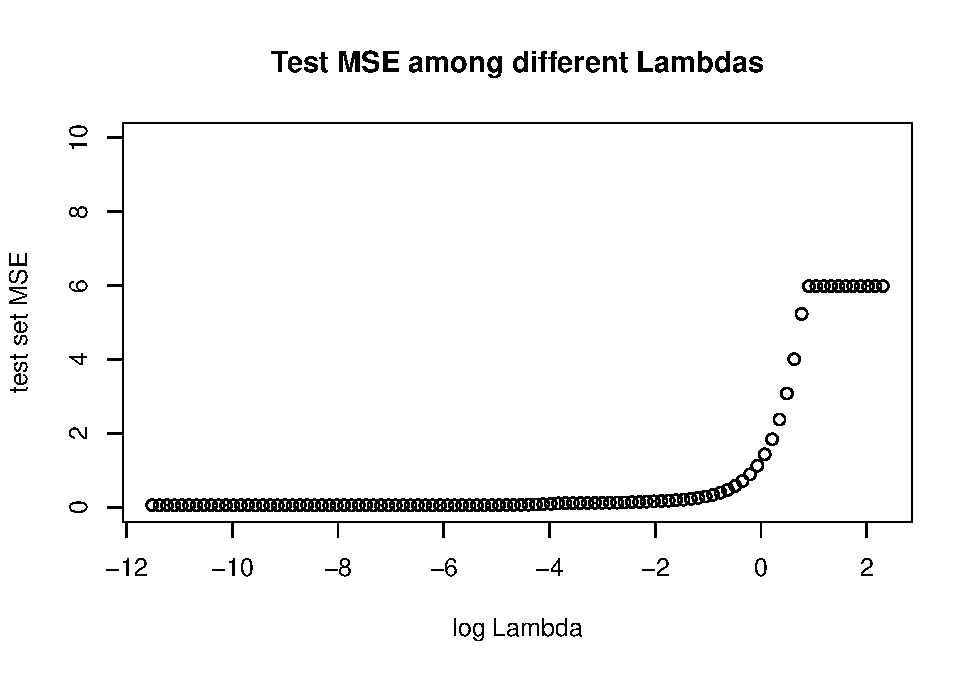
\includegraphics{TSLproject_files/figure-latex/unnamed-chunk-17-1.pdf}

\begin{Shaded}
\begin{Highlighting}[]
\NormalTok{bestlam =}\StringTok{ }\NormalTok{grid[}\KeywordTok{which.min}\NormalTok{(err.i)]}
\KeywordTok{points}\NormalTok{(}\KeywordTok{log}\NormalTok{(grid)[bestlam], err.i[bestlam], }\DataTypeTok{col =}\StringTok{"red"}\NormalTok{, }\DataTypeTok{cex=}\DecValTok{2}\NormalTok{, }\DataTypeTok{pch=}\DecValTok{20}\NormalTok{)}
\end{Highlighting}
\end{Shaded}

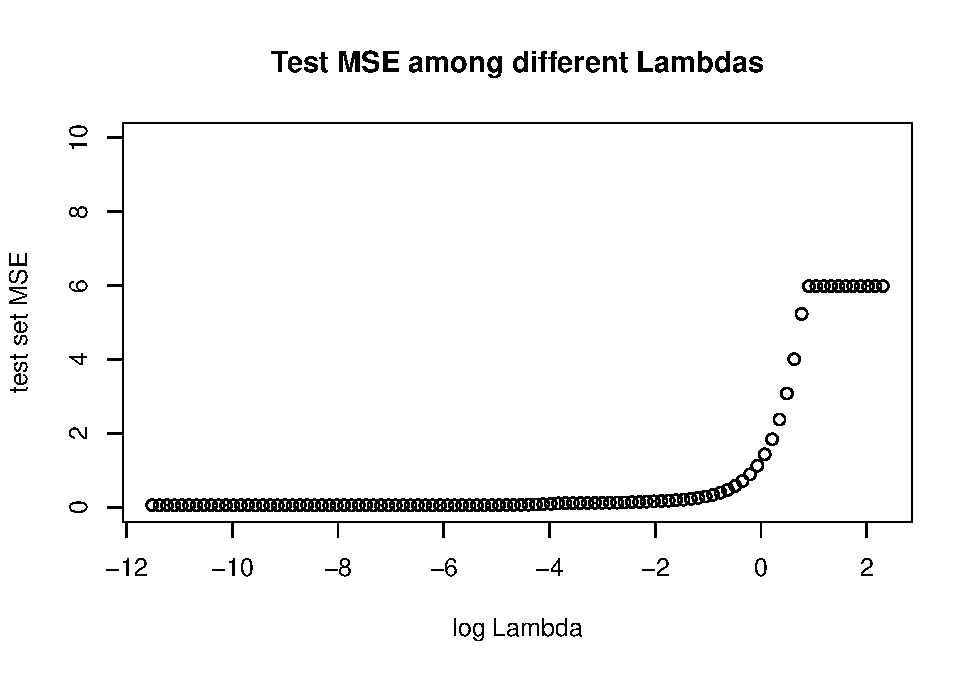
\includegraphics{TSLproject_files/figure-latex/unnamed-chunk-17-2.pdf}

\begin{Shaded}
\begin{Highlighting}[]
\CommentTok{# high values of lambda are like fitting just the intercept}

\CommentTok{# using 10 folds CV}
\KeywordTok{set.seed}\NormalTok{ (}\DecValTok{1}\NormalTok{)}
\NormalTok{cv.out =}\StringTok{ }\KeywordTok{cv.glmnet}\NormalTok{(x[train ,], y[train], }\DataTypeTok{alpha =} \DecValTok{1}\NormalTok{)}
\KeywordTok{plot}\NormalTok{(cv.out)}
\end{Highlighting}
\end{Shaded}

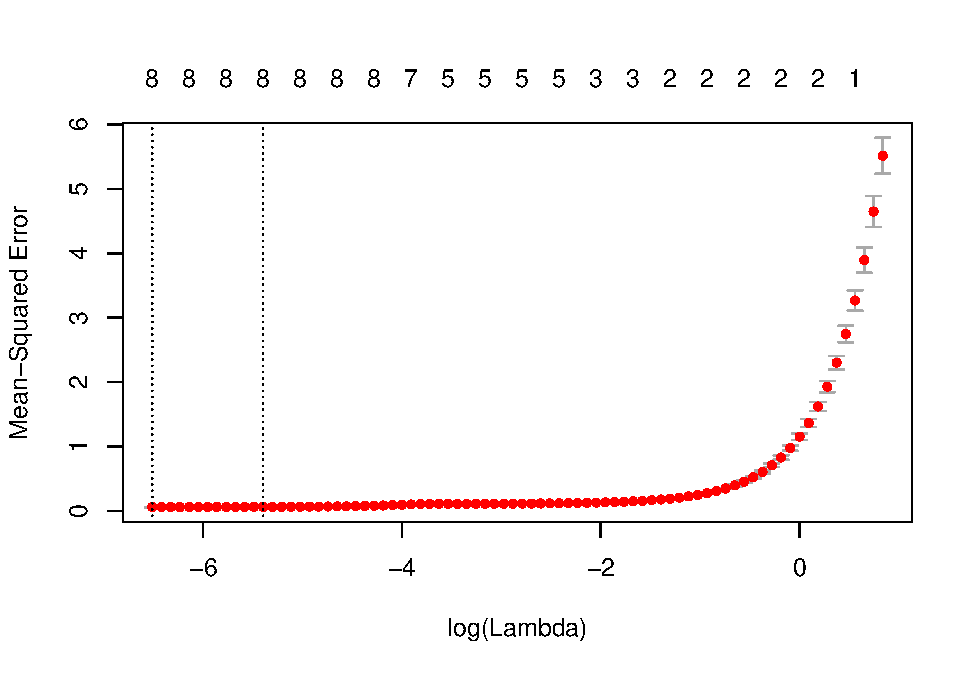
\includegraphics{TSLproject_files/figure-latex/unnamed-chunk-17-3.pdf}

\begin{Shaded}
\begin{Highlighting}[]
\NormalTok{bestlam =}\StringTok{ }\NormalTok{cv.out}\OperatorTok{$}\NormalTok{lambda.min}
\NormalTok{bestlam}
\end{Highlighting}
\end{Shaded}

\begin{verbatim}
## [1] 0.001484687
\end{verbatim}

\begin{Shaded}
\begin{Highlighting}[]
\NormalTok{lasso.pred =}\StringTok{ }\KeywordTok{predict}\NormalTok{(lasso.mod, }\DataTypeTok{s=}\NormalTok{bestlam, }\DataTypeTok{newx=}\NormalTok{x[test ,])}
\KeywordTok{mean}\NormalTok{((lasso.pred }\OperatorTok{-}\StringTok{ }\NormalTok{y.test)}\OperatorTok{^}\DecValTok{2}\NormalTok{)}
\end{Highlighting}
\end{Shaded}

\begin{verbatim}
## [1] 0.05322848
\end{verbatim}

\begin{Shaded}
\begin{Highlighting}[]
\CommentTok{# using best subset}
\KeywordTok{require}\NormalTok{(leaps)}
\end{Highlighting}
\end{Shaded}

\begin{verbatim}
## Loading required package: leaps
\end{verbatim}

\begin{Shaded}
\begin{Highlighting}[]
\NormalTok{dataBS =}\StringTok{ }\KeywordTok{as.data.frame}\NormalTok{(}\KeywordTok{cbind}\NormalTok{(y, x))}
\NormalTok{best.sub =}\StringTok{ }\KeywordTok{regsubsets}\NormalTok{(y }\OperatorTok{~}\StringTok{ }\NormalTok{x, }\DataTypeTok{data =}\NormalTok{ dataBS, }\DataTypeTok{nvmax =} \KeywordTok{nrow}\NormalTok{(}\KeywordTok{coef}\NormalTok{(lasso.mod)))}
\NormalTok{best.sub.summary =}\StringTok{ }\KeywordTok{summary}\NormalTok{(best.sub)}
\KeywordTok{names}\NormalTok{(best.sub.summary)}
\end{Highlighting}
\end{Shaded}

\begin{verbatim}
## [1] "which"  "rsq"    "rss"    "adjr2"  "cp"     "bic"    "outmat" "obj"
\end{verbatim}

\begin{Shaded}
\begin{Highlighting}[]
\CommentTok{# manual plotting}
\KeywordTok{par}\NormalTok{(}\DataTypeTok{mfrow =}\KeywordTok{c}\NormalTok{(}\DecValTok{2}\NormalTok{,}\DecValTok{2}\NormalTok{))}
\CommentTok{# rsq}
\KeywordTok{plot}\NormalTok{(best.sub.summary}\OperatorTok{$}\NormalTok{rsq , }\DataTypeTok{xlab=}\StringTok{"Number of Variables"}\NormalTok{, }\DataTypeTok{ylab=}\StringTok{"Rsq"}\NormalTok{, }\DataTypeTok{type=}\StringTok{"l"}\NormalTok{)}
\NormalTok{ind_Rsq =}\StringTok{ }\KeywordTok{which.max}\NormalTok{(best.sub.summary}\OperatorTok{$}\NormalTok{rsq)}
\KeywordTok{points}\NormalTok{(ind_Rsq, best.sub.summary}\OperatorTok{$}\NormalTok{adjr2[ind_Rsq], }\DataTypeTok{col =}\StringTok{"red"}\NormalTok{, }\DataTypeTok{cex=}\DecValTok{2}\NormalTok{, }\DataTypeTok{pch=}\DecValTok{20}\NormalTok{)}
\CommentTok{# adjRsq}
\KeywordTok{plot}\NormalTok{(best.sub.summary}\OperatorTok{$}\NormalTok{adjr2 ,}\DataTypeTok{xlab=}\StringTok{"Number of Variables"}\NormalTok{, }\DataTypeTok{ylab=}\StringTok{"Adjusted RSq"}\NormalTok{, }\DataTypeTok{type=}\StringTok{"l"}\NormalTok{)}
\NormalTok{ind_adjRsq =}\StringTok{ }\KeywordTok{which.max}\NormalTok{(best.sub.summary}\OperatorTok{$}\NormalTok{adjr2)}
\KeywordTok{points}\NormalTok{(ind_adjRsq, best.sub.summary}\OperatorTok{$}\NormalTok{adjr2[ind_adjRsq], }\DataTypeTok{col =}\StringTok{"red"}\NormalTok{, }\DataTypeTok{cex=}\DecValTok{2}\NormalTok{, }\DataTypeTok{pch=}\DecValTok{20}\NormalTok{)}
\CommentTok{# Cp}
\KeywordTok{plot}\NormalTok{(best.sub.summary}\OperatorTok{$}\NormalTok{cp ,}\DataTypeTok{xlab=}\StringTok{"Number of Variables"}\NormalTok{, }\DataTypeTok{ylab=}\StringTok{"Cp"}\NormalTok{, }\DataTypeTok{type=}\StringTok{"l"}\NormalTok{)}
\NormalTok{ind_Cp =}\StringTok{ }\KeywordTok{which.min}\NormalTok{(best.sub.summary}\OperatorTok{$}\NormalTok{cp)}
\KeywordTok{points}\NormalTok{(ind_Cp, best.sub.summary}\OperatorTok{$}\NormalTok{cp[ind_adjRsq], }\DataTypeTok{col =}\StringTok{"red"}\NormalTok{, }\DataTypeTok{cex=}\DecValTok{2}\NormalTok{, }\DataTypeTok{pch=}\DecValTok{20}\NormalTok{)}
\CommentTok{# bic}
\KeywordTok{plot}\NormalTok{(best.sub.summary}\OperatorTok{$}\NormalTok{bic ,}\DataTypeTok{xlab=}\StringTok{"Number of Variables"}\NormalTok{, }\DataTypeTok{ylab=}\StringTok{"bic"}\NormalTok{, }\DataTypeTok{type=}\StringTok{"l"}\NormalTok{)}
\end{Highlighting}
\end{Shaded}

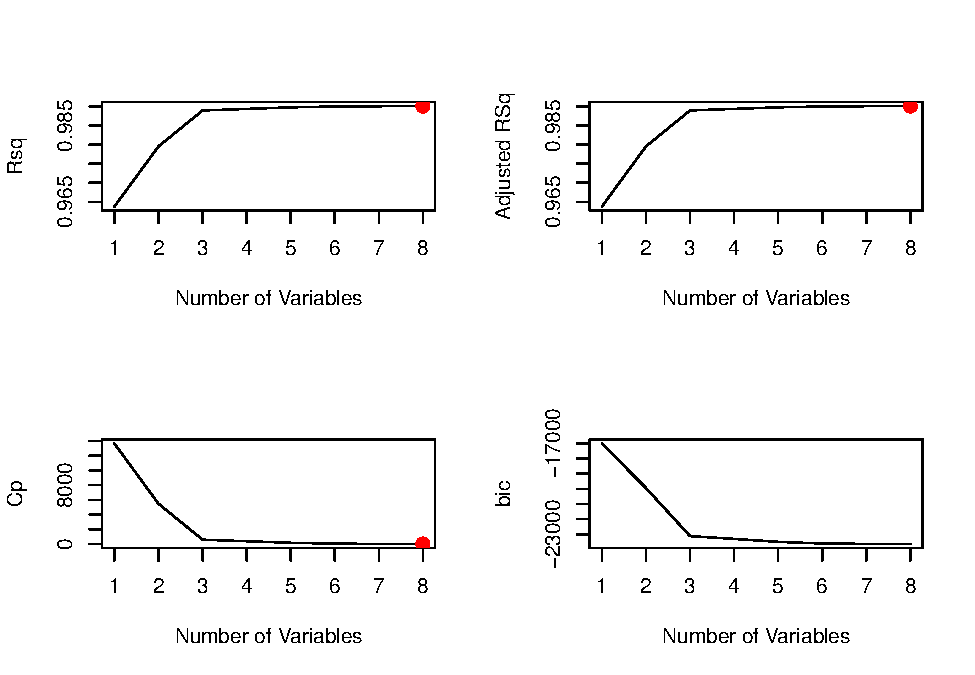
\includegraphics{TSLproject_files/figure-latex/unnamed-chunk-17-4.pdf}

\begin{Shaded}
\begin{Highlighting}[]
\NormalTok{ind_bic =}\StringTok{ }\KeywordTok{which.min}\NormalTok{(best.sub.summary}\OperatorTok{$}\NormalTok{bic)}
\KeywordTok{points}\NormalTok{(ind_bic, best.sub.summary}\OperatorTok{$}\NormalTok{bic[ind_bic], }\DataTypeTok{col =}\StringTok{"red"}\NormalTok{, }\DataTypeTok{cex=}\DecValTok{2}\NormalTok{, }\DataTypeTok{pch=}\DecValTok{20}\NormalTok{)}
\end{Highlighting}
\end{Shaded}

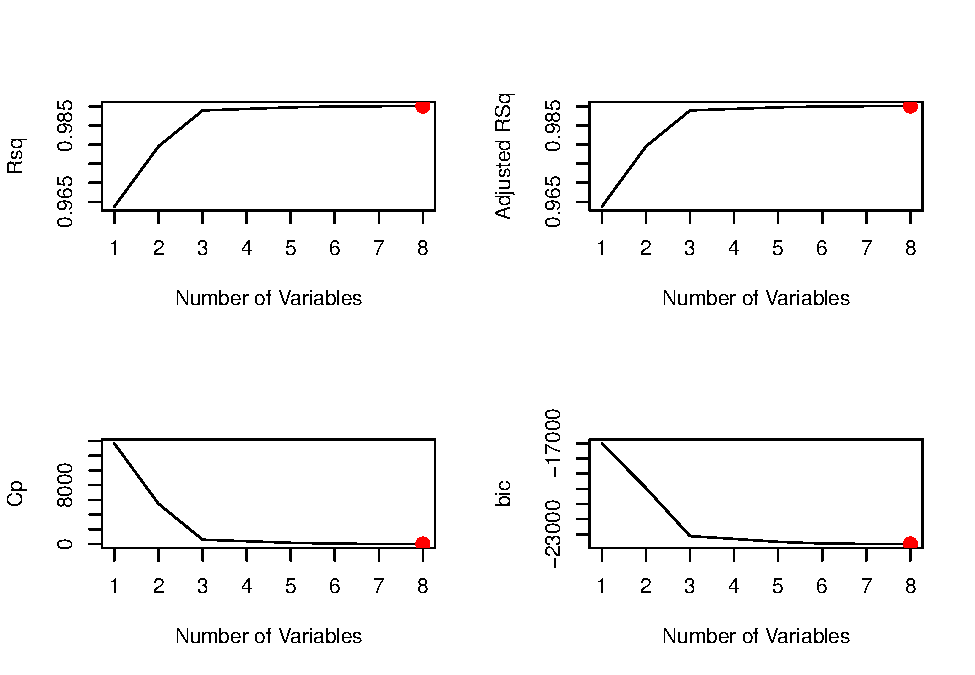
\includegraphics{TSLproject_files/figure-latex/unnamed-chunk-17-5.pdf}

\begin{Shaded}
\begin{Highlighting}[]
\CommentTok{# built-in plots}
\NormalTok{?plot.regsubsets}
\end{Highlighting}
\end{Shaded}

\begin{verbatim}
## starting httpd help server ...
\end{verbatim}

\begin{verbatim}
##  done
\end{verbatim}

\begin{Shaded}
\begin{Highlighting}[]
\KeywordTok{par}\NormalTok{(}\DataTypeTok{mfrow=}\KeywordTok{c}\NormalTok{(}\DecValTok{1}\NormalTok{,}\DecValTok{1}\NormalTok{))}
\KeywordTok{plot}\NormalTok{(best.sub, }\DataTypeTok{scale =} \StringTok{"r2"}\NormalTok{)}
\end{Highlighting}
\end{Shaded}

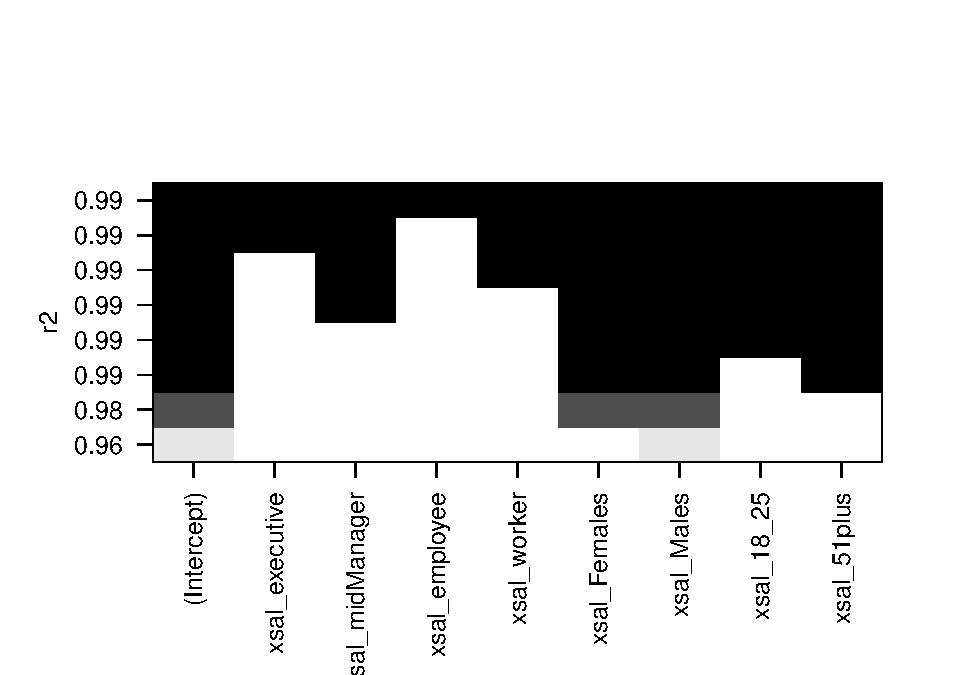
\includegraphics{TSLproject_files/figure-latex/unnamed-chunk-17-6.pdf}

\begin{Shaded}
\begin{Highlighting}[]
\KeywordTok{plot}\NormalTok{(best.sub, }\DataTypeTok{scale =} \StringTok{"adjr2"}\NormalTok{)}
\end{Highlighting}
\end{Shaded}

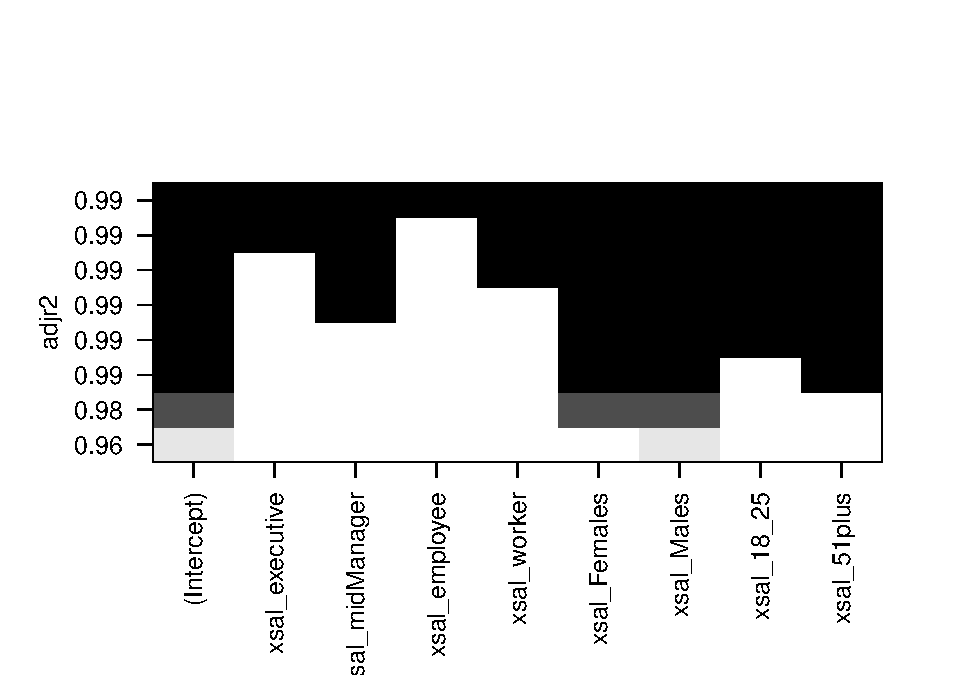
\includegraphics{TSLproject_files/figure-latex/unnamed-chunk-17-7.pdf}

\begin{Shaded}
\begin{Highlighting}[]
\KeywordTok{plot}\NormalTok{(best.sub, }\DataTypeTok{scale =} \StringTok{"Cp"}\NormalTok{)}
\end{Highlighting}
\end{Shaded}

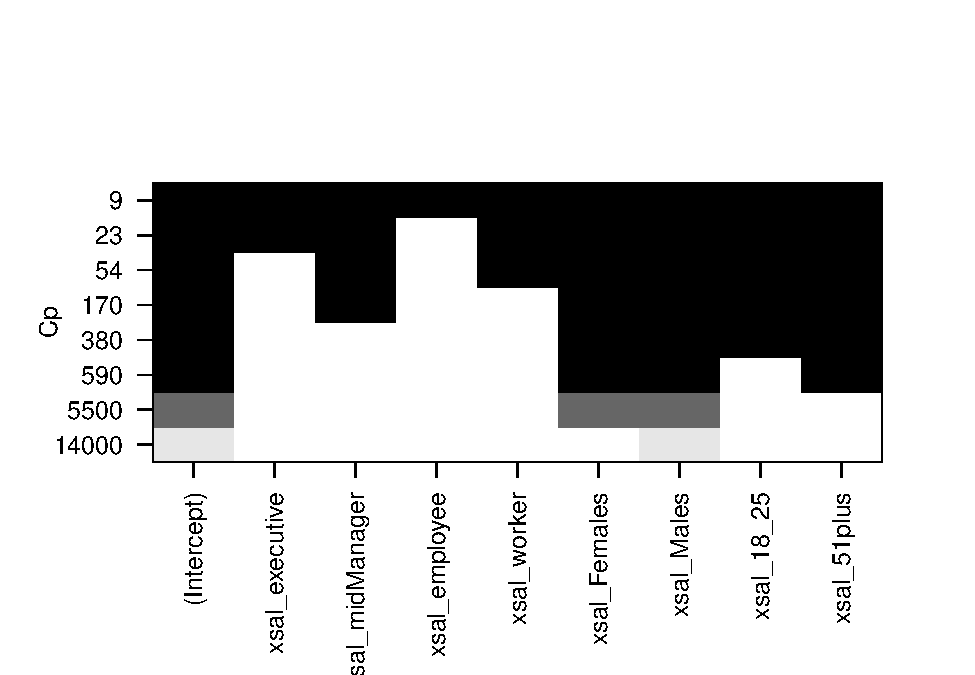
\includegraphics{TSLproject_files/figure-latex/unnamed-chunk-17-8.pdf}

\begin{Shaded}
\begin{Highlighting}[]
\KeywordTok{plot}\NormalTok{(best.sub, }\DataTypeTok{scale =} \StringTok{"bic"}\NormalTok{)}
\end{Highlighting}
\end{Shaded}

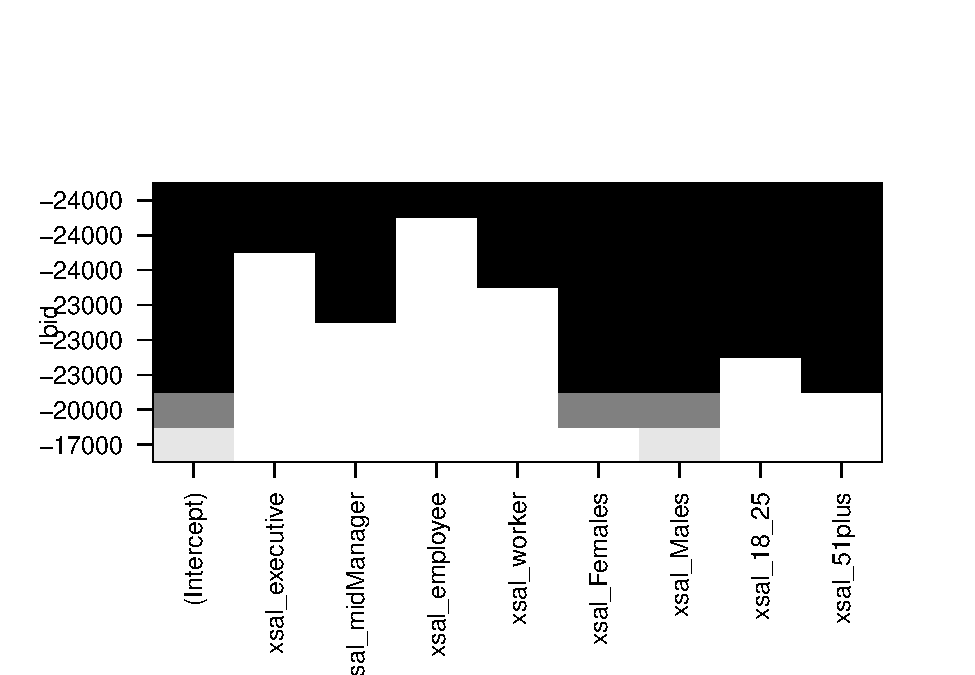
\includegraphics{TSLproject_files/figure-latex/unnamed-chunk-17-9.pdf}

\begin{Shaded}
\begin{Highlighting}[]
\CommentTok{# retrieve the model with min BIC}
\KeywordTok{coefficients}\NormalTok{(best.sub, }\KeywordTok{which.min}\NormalTok{(best.sub.summary}\OperatorTok{$}\NormalTok{bic))}
\end{Highlighting}
\end{Shaded}

\begin{verbatim}
##     (Intercept)  xsal_executive xsal_midManager   xsal_employee 
##     -0.25048976     -0.01269488      0.04760461      0.04132812 
##     xsal_worker    xsal_Females      xsal_Males      xsal_18_25 
##      0.04170107      0.56842466      0.73332696     -0.07044077 
##     xsal_51plus 
##     -0.29040179
\end{verbatim}

Model salaries for people aged 18-25, which seems more difficult to
predict:

\begin{Shaded}
\begin{Highlighting}[]
\KeywordTok{plot}\NormalTok{(}\DataTypeTok{y =}\NormalTok{ salary}\OperatorTok{$}\NormalTok{sal_18_}\DecValTok{25}\NormalTok{, }\DataTypeTok{x =}\NormalTok{ salary}\OperatorTok{$}\NormalTok{sal_51plus)}
\end{Highlighting}
\end{Shaded}

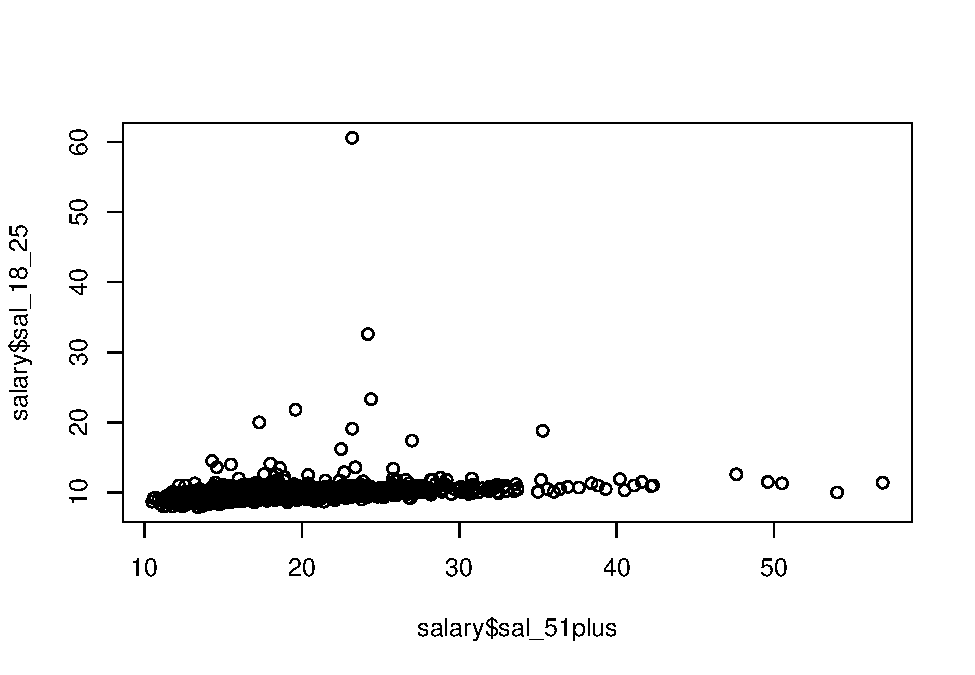
\includegraphics{TSLproject_files/figure-latex/unnamed-chunk-18-1.pdf}

\begin{Shaded}
\begin{Highlighting}[]
\CommentTok{# there is a clear outlier}
\NormalTok{ind_out =}\StringTok{ }\KeywordTok{which}\NormalTok{(salary}\OperatorTok{$}\NormalTok{sal_18_}\DecValTok{25} \OperatorTok{==}\StringTok{ }\KeywordTok{max}\NormalTok{(salary}\OperatorTok{$}\NormalTok{sal_18_}\DecValTok{25}\NormalTok{))}
\CommentTok{# check if is so in all dimensions (apparently not)}
\NormalTok{col_col <-}\StringTok{ }\KeywordTok{rep}\NormalTok{(}\StringTok{"black"}\NormalTok{, }\KeywordTok{nrow}\NormalTok{(salary))}
\NormalTok{col_col[ind_out] <-}\StringTok{ "red"}
\KeywordTok{pairs}\NormalTok{(salary[, }\KeywordTok{c}\NormalTok{(}\DecValTok{3}\OperatorTok{:}\DecValTok{8}\NormalTok{, }\DecValTok{13}\NormalTok{, }\DecValTok{18}\OperatorTok{:}\DecValTok{20}\NormalTok{)], }\DataTypeTok{col =}\NormalTok{ col_col)}
\end{Highlighting}
\end{Shaded}

\includegraphics{TSLproject_files/figure-latex/unnamed-chunk-18-2.pdf}

\begin{Shaded}
\begin{Highlighting}[]
\CommentTok{# evaluate an OLS fit}
\NormalTok{fit_LM_18_}\DecValTok{25}\NormalTok{ =}\StringTok{ }\KeywordTok{lm}\NormalTok{(salary}\OperatorTok{$}\NormalTok{sal_18_}\DecValTok{25} \OperatorTok{~}\StringTok{ }\NormalTok{salary}\OperatorTok{$}\NormalTok{sal_51plus)}
\KeywordTok{plot}\NormalTok{(}\DataTypeTok{y =}\NormalTok{ salary}\OperatorTok{$}\NormalTok{sal_18_}\DecValTok{25}\NormalTok{, }\DataTypeTok{x =}\NormalTok{ salary}\OperatorTok{$}\NormalTok{sal_51plus)}
\end{Highlighting}
\end{Shaded}

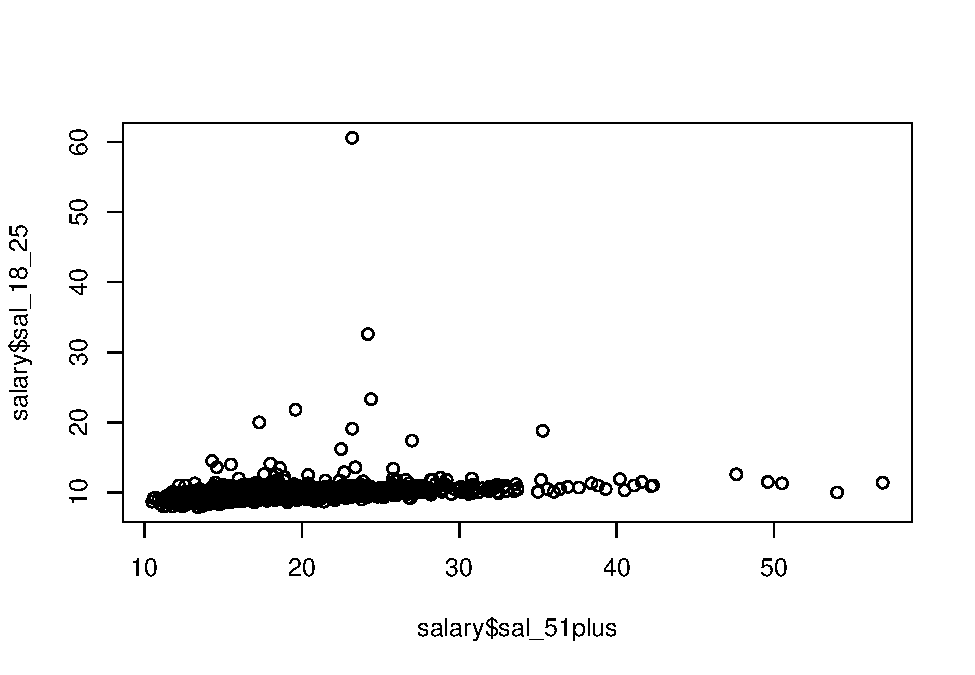
\includegraphics{TSLproject_files/figure-latex/unnamed-chunk-18-3.pdf}

\begin{Shaded}
\begin{Highlighting}[]
\KeywordTok{abline}\NormalTok{(fit_LM_18_}\DecValTok{25}\NormalTok{, }\DataTypeTok{lwd=}\DecValTok{3}\NormalTok{, }\DataTypeTok{col=}\StringTok{"red"}\NormalTok{)}
\end{Highlighting}
\end{Shaded}

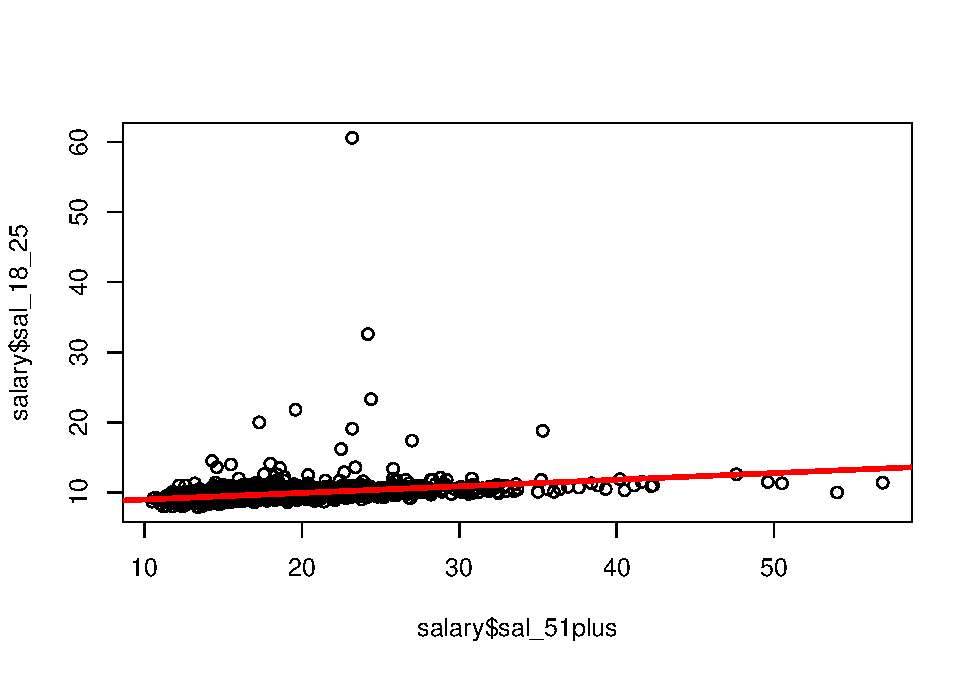
\includegraphics{TSLproject_files/figure-latex/unnamed-chunk-18-4.pdf}

\begin{Shaded}
\begin{Highlighting}[]
\CommentTok{# # using more predictors}
\CommentTok{# fit_LM_2 = lm(salary$sal_M_18_25 ~ salary$sal_26_50 + salary$sal_51plus + salary$sal_general + salary$sal_executive + }
\CommentTok{#                 salary$sal_midManager + salary$sal_employee + salary$sal_worker)}
\CommentTok{# }
\CommentTok{# summary(fit_LM_2)}
\end{Highlighting}
\end{Shaded}

PCA for salary:

\begin{Shaded}
\begin{Highlighting}[]
\NormalTok{myPr <-}\StringTok{ }\KeywordTok{prcomp}\NormalTok{(salary[, }\DecValTok{3}\OperatorTok{:}\DecValTok{26}\NormalTok{], }\DataTypeTok{scale =} \OtherTok{TRUE}\NormalTok{)}
\NormalTok{myPr}
\end{Highlighting}
\end{Shaded}

\begin{verbatim}
## Standard deviations (1, .., p=24):
##  [1] 4.06846384 1.42984463 1.05721988 1.01203703 0.88322482 0.75520781
##  [7] 0.66774657 0.62302595 0.59239652 0.54263890 0.42693995 0.34427033
## [13] 0.24469681 0.18858814 0.09684001 0.08031760 0.07067011 0.06516261
## [19] 0.05970587 0.05220597 0.04552586 0.03013818 0.02484499 0.01231068
## 
## Rotation (n x k) = (24 x 24):
##                         PC1          PC2          PC3          PC4
## sal_general      0.24256129  0.025437648  0.046824213 -0.001482692
## sal_executive    0.20442703  0.090840110  0.370504255  0.230155704
## sal_midManager   0.18190516 -0.298541632  0.240776890 -0.140328052
## sal_employee     0.22422720  0.071074352 -0.247268798 -0.004042860
## sal_worker       0.20363449  0.025689939 -0.009919171 -0.462312126
## sal_Females      0.23675441  0.077421630 -0.127192423  0.117888907
## sal_F_executive  0.17552119  0.100201572  0.134347070  0.360580387
## sal_F_midManager 0.20157041  0.055250814 -0.153976516  0.149031116
## sal_F_employee   0.21685115  0.070759163 -0.278486962  0.062336516
## sal_F_worker     0.17716298  0.057667740 -0.157481946 -0.339303819
## sal_Males        0.23974996  0.009058135  0.108615013 -0.027686738
## sal_M_executive  0.19790649  0.083491339  0.384046886  0.195161560
## sal_M_midManager 0.15142477 -0.358343778  0.337293684 -0.200802616
## sal_M_employee   0.18899143  0.053355476 -0.169087541 -0.135169015
## sal_M_worker     0.19759147  0.020542131  0.014779054 -0.466418793
## sal_18_25        0.10622764 -0.581187020 -0.184539817  0.163255107
## sal_26_50        0.24075123  0.021743461  0.009686478 -0.023148467
## sal_51plus       0.23674140  0.067331626  0.096987533  0.053894395
## sal_F_18_25      0.15872871 -0.016579718 -0.401651320  0.127716025
## sal_F_26_50      0.23464487  0.070413931 -0.134126680  0.098562960
## sal_F_51plus     0.22653207  0.089063623 -0.110555475  0.170095574
## sal_M_18_25      0.08512445 -0.608375999 -0.120979871  0.149766048
## sal_M_26_50      0.23769037  0.003296056  0.072159424 -0.061623773
## sal_M_51plus     0.23172375  0.063471847  0.155656542  0.046627399
##                          PC5         PC6          PC7          PC8
## sal_general       0.03076820 -0.06451689  0.055294659 -0.109456636
## sal_executive     0.21350371  0.06702947  0.104690622  0.145407429
## sal_midManager   -0.46401004  0.11032025 -0.039816322  0.040856787
## sal_employee     -0.12740320 -0.26329990  0.014366575  0.145665182
## sal_worker        0.22036076  0.13598966 -0.117636498  0.083375097
## sal_Females      -0.04566119 -0.00897671 -0.086720278 -0.154060756
## sal_F_executive   0.05685253  0.19723908 -0.624677246  0.515695940
## sal_F_midManager -0.30014668  0.08207409 -0.170354268 -0.244385975
## sal_F_employee   -0.16747839 -0.07036376 -0.061129067 -0.068005412
## sal_F_worker      0.23212123  0.26673263 -0.223203762 -0.157579547
## sal_Males         0.05507451 -0.09080437  0.109670620 -0.104435046
## sal_M_executive   0.22445421  0.03841633  0.283820931  0.005970518
## sal_M_midManager -0.45538809  0.09851366  0.008813757  0.102547206
## sal_M_employee   -0.04337624 -0.57642720  0.149112333  0.540346236
## sal_M_worker      0.22279564  0.11403974 -0.098836166  0.127142364
## sal_18_25         0.26393156 -0.01583997  0.002640546  0.001207696
## sal_26_50        -0.01895745 -0.07602419  0.036997646 -0.096505574
## sal_51plus        0.06972164 -0.03408813  0.097629771 -0.145711593
## sal_F_18_25      -0.07694791  0.60485366  0.529432039  0.330226773
## sal_F_26_50      -0.03913166 -0.02936739 -0.075060725 -0.157937046
## sal_F_51plus     -0.07331241  0.01993173 -0.147758727 -0.179672634
## sal_M_18_25       0.29054243 -0.13104749 -0.094878245 -0.061587053
## sal_M_26_50      -0.01062363 -0.10331821  0.086592887 -0.080401426
## sal_M_51plus      0.10720803 -0.05185343  0.173774628 -0.146634702
##                           PC9        PC10         PC11         PC12
## sal_general       0.027674801 -0.17031410  0.080977040 -0.072080349
## sal_executive    -0.095281235  0.27788374 -0.116184031 -0.091277662
## sal_midManager   -0.057858294  0.09569372  0.035330196  0.042527735
## sal_employee     -0.024675374  0.13257444 -0.327104176  0.043849057
## sal_worker        0.292638010  0.11437721 -0.009936159  0.020419566
## sal_Females       0.014970640 -0.13019350 -0.005154802 -0.052074804
## sal_F_executive   0.024647934 -0.19920315  0.053743470 -0.029629692
## sal_F_midManager  0.109517724  0.61073768  0.498058587 -0.074307675
## sal_F_employee    0.061094057  0.15347166 -0.656257011 -0.053673559
## sal_F_worker     -0.777224505  0.05063640  0.007552204  0.066475744
## sal_Males         0.018817088 -0.18588939  0.102679421 -0.081239041
## sal_M_executive  -0.115734021  0.37274958 -0.172453447 -0.060289875
## sal_M_midManager -0.109776798 -0.12475279 -0.157598363  0.077146650
## sal_M_employee   -0.219903667  0.08926476  0.293843520  0.121124001
## sal_M_worker      0.436609055  0.12512635 -0.024954387 -0.004215415
## sal_18_25         0.023279317  0.04512387  0.017294431  0.002633665
## sal_26_50         0.002769069 -0.20498532  0.073845015 -0.364981228
## sal_51plus        0.074302719 -0.14219097  0.075553331  0.399980948
## sal_F_18_25       0.021573772 -0.10397906  0.086328029 -0.000224029
## sal_F_26_50       0.005991692 -0.15389749 -0.003958265 -0.313921974
## sal_F_51plus      0.072336569 -0.10300216 -0.029610665  0.522101524
## sal_M_18_25       0.020934887  0.05728994  0.001050080  0.009639714
## sal_M_26_50      -0.008463477 -0.22436907  0.096794152 -0.380087545
## sal_M_51plus      0.053171099 -0.15006742  0.092894490  0.355160148
##                          PC13         PC14        PC15         PC16
## sal_general       0.034011467 -0.087574401  0.11373308  0.537564433
## sal_executive    -0.050262712 -0.094749290  0.21491568  0.036365780
## sal_midManager    0.048701263  0.007430303  0.63673058 -0.057984682
## sal_employee      0.101729065 -0.054861091 -0.07035113  0.067292007
## sal_worker       -0.067190044  0.073124691  0.06597172  0.060818933
## sal_Females      -0.166052462  0.362943040 -0.03857624  0.369567679
## sal_F_executive   0.150284303 -0.070732588 -0.07123694 -0.015017006
## sal_F_midManager  0.125149260 -0.106259680 -0.21693732  0.007488834
## sal_F_employee    0.217741396 -0.203891674  0.02547217 -0.043943649
## sal_F_worker      0.056051310 -0.048241531 -0.01598948 -0.019478631
## sal_Males         0.098859708 -0.255477734 -0.16183855  0.397833221
## sal_M_executive  -0.220371258  0.201825172 -0.15473575 -0.031433765
## sal_M_midManager -0.065776558  0.139626301 -0.52596569  0.054175552
## sal_M_employee   -0.091199655  0.106345961  0.02179142 -0.032252775
## sal_M_worker     -0.041622685  0.045210768 -0.07283739 -0.075671203
## sal_18_25         0.013002070 -0.016293108  0.11267039  0.136111542
## sal_26_50        -0.100043127 -0.098288179  0.15596215 -0.240473153
## sal_51plus        0.234263596  0.011064433  0.20197212 -0.010017352
## sal_F_18_25      -0.008227617 -0.025813810 -0.02877802 -0.022084438
## sal_F_26_50       0.039401540  0.651433643  0.07061276 -0.232593633
## sal_F_51plus     -0.660491905 -0.132164963  0.01971171 -0.153288200
## sal_M_18_25      -0.004391171 -0.001068603 -0.11587697 -0.154164465
## sal_M_26_50      -0.163926845 -0.432693213 -0.12254212 -0.331702528
## sal_M_51plus      0.510074815  0.066303930 -0.16311384 -0.318822068
##                         PC17         PC18          PC19         PC20
## sal_general       0.02743203  0.017489988 -1.159451e-01 -0.004941698
## sal_executive     0.60389368  0.183292088  1.113154e-02  0.209707749
## sal_midManager   -0.28448202 -0.073557676 -1.579773e-01  0.048891526
## sal_employee      0.17510667 -0.754946928 -1.146551e-01  0.037348700
## sal_worker        0.11187552  0.010201055  1.064764e-01 -0.667777877
## sal_Females      -0.11208987  0.081286141  2.356819e-02  0.155294284
## sal_F_executive  -0.15296912 -0.053925877  2.295057e-05 -0.068963399
## sal_F_midManager  0.07002096  0.014105017  4.580890e-02 -0.026142503
## sal_F_employee   -0.14364839  0.483278945  7.405760e-02 -0.061767647
## sal_F_worker     -0.01489252 -0.012757413 -1.294547e-02  0.078849344
## sal_Males        -0.16104495  0.065851739 -1.876303e-01  0.002719009
## sal_M_executive  -0.48853916 -0.147678103 -1.172190e-02 -0.169556473
## sal_M_midManager  0.25541377  0.073609475  1.327127e-01 -0.021557735
## sal_M_employee   -0.05884846  0.283858888  4.685199e-02 -0.008460942
## sal_M_worker     -0.09758683  0.006946048 -8.677017e-02  0.610432699
## sal_18_25        -0.07112277 -0.109030858  6.634365e-01  0.107558876
## sal_26_50         0.12380994 -0.080862049  6.569177e-02 -0.023716404
## sal_51plus        0.19641903 -0.041589840  3.230681e-02 -0.164704064
## sal_F_18_25       0.01487853  0.017465862 -1.179785e-01 -0.021515015
## sal_F_26_50       0.12772260  0.028461809 -2.675494e-02 -0.014024159
## sal_F_51plus      0.01638906  0.022108181 -5.690660e-04  0.043471311
## sal_M_18_25       0.07360042  0.100079168 -6.191465e-01 -0.107431569
## sal_M_26_50      -0.09163891 -0.056093094  1.197454e-01 -0.039867540
## sal_M_51plus     -0.12772664  0.009630106  9.046612e-02  0.099182609
##                          PC21         PC22         PC23          PC24
## sal_general      -0.186444087 -0.171634618 -0.318250742 -0.6211947949
## sal_executive     0.237625932  0.094261014  0.051498899 -0.0009957993
## sal_midManager    0.145407708  0.074636362  0.046910335 -0.0028543575
## sal_employee      0.097556946  0.039721344  0.018583473 -0.0002310930
## sal_worker        0.259563686  0.033684544 -0.025598837 -0.0021445691
## sal_Females       0.414226899 -0.405780691  0.378673412  0.1835641555
## sal_F_executive  -0.063321530 -0.024249456 -0.013372003  0.0009117450
## sal_F_midManager -0.058101242 -0.025079710 -0.016977172  0.0013027139
## sal_F_employee   -0.087559551 -0.033287099 -0.022210938  0.0014008536
## sal_F_worker     -0.040868629 -0.004198171  0.001678796  0.0003570630
## sal_Males         0.045217001  0.551474149 -0.042726401  0.4589400496
## sal_M_executive  -0.197052690 -0.077600321 -0.040965609  0.0010058968
## sal_M_midManager -0.109754841 -0.056017369 -0.034265555  0.0021278696
## sal_M_employee   -0.035280604 -0.011036698 -0.007791783 -0.0002416376
## sal_M_worker     -0.203024554 -0.024335767  0.030257103  0.0025064712
## sal_18_25        -0.034850157  0.119248356 -0.037628737  0.0160530627
## sal_26_50        -0.117863633 -0.419501092 -0.475425046  0.4460448356
## sal_51plus       -0.540731132 -0.144167569  0.439057354  0.1690205439
## sal_F_18_25       0.001253538 -0.008376178  0.002582028 -0.0034582040
## sal_F_26_50      -0.150941457  0.456530696 -0.027601748 -0.1483871402
## sal_F_51plus      0.035742420  0.177587916 -0.187687161 -0.0459163395
## sal_M_18_25       0.032360802 -0.129213299  0.043266374 -0.0149062160
## sal_M_26_50       0.095574005  0.028289510  0.477463900 -0.3177600192
## sal_M_51plus      0.430473611 -0.062171646 -0.238321858 -0.1290375524
\end{verbatim}

\begin{Shaded}
\begin{Highlighting}[]
\KeywordTok{summary}\NormalTok{(myPr)}
\end{Highlighting}
\end{Shaded}

\begin{verbatim}
## Importance of components:
##                           PC1     PC2     PC3     PC4    PC5     PC6
## Standard deviation     4.0685 1.42984 1.05722 1.01204 0.8832 0.75521
## Proportion of Variance 0.6897 0.08519 0.04657 0.04268 0.0325 0.02376
## Cumulative Proportion  0.6897 0.77487 0.82144 0.86412 0.8966 0.92038
##                            PC7     PC8     PC9    PC10    PC11    PC12
## Standard deviation     0.66775 0.62303 0.59240 0.54264 0.42694 0.34427
## Proportion of Variance 0.01858 0.01617 0.01462 0.01227 0.00759 0.00494
## Cumulative Proportion  0.93896 0.95514 0.96976 0.98203 0.98962 0.99456
##                           PC13    PC14    PC15    PC16    PC17    PC18
## Standard deviation     0.24470 0.18859 0.09684 0.08032 0.07067 0.06516
## Proportion of Variance 0.00249 0.00148 0.00039 0.00027 0.00021 0.00018
## Cumulative Proportion  0.99706 0.99854 0.99893 0.99920 0.99940 0.99958
##                           PC19    PC20    PC21    PC22    PC23    PC24
## Standard deviation     0.05971 0.05221 0.04553 0.03014 0.02484 0.01231
## Proportion of Variance 0.00015 0.00011 0.00009 0.00004 0.00003 0.00001
## Cumulative Proportion  0.99973 0.99984 0.99993 0.99997 0.99999 1.00000
\end{verbatim}

\begin{Shaded}
\begin{Highlighting}[]
\KeywordTok{plot}\NormalTok{(myPr, }\DataTypeTok{type =} \StringTok{"l"}\NormalTok{)}
\end{Highlighting}
\end{Shaded}

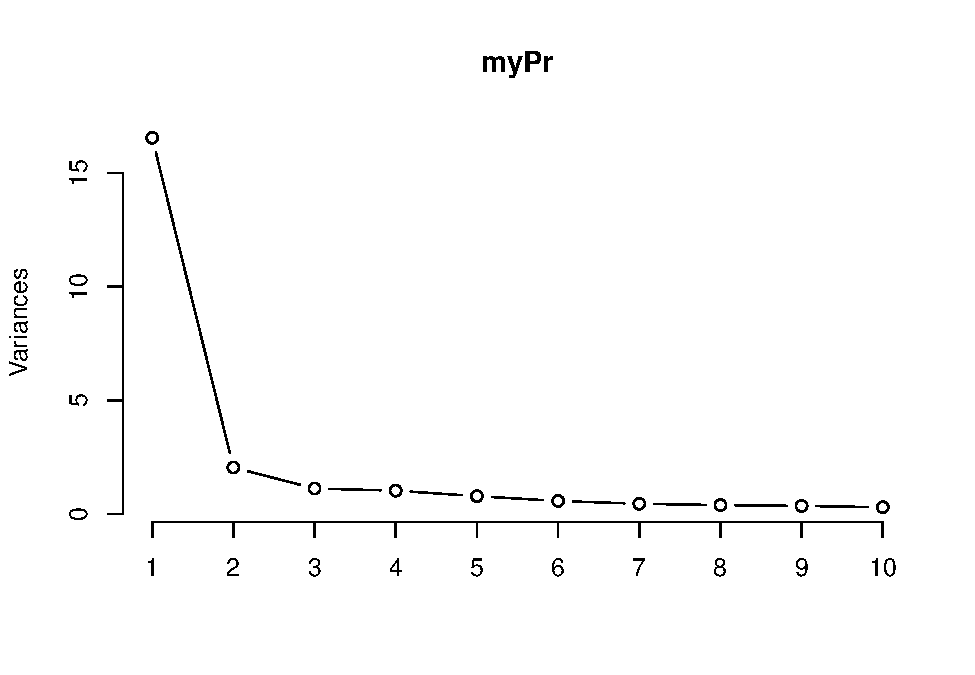
\includegraphics{TSLproject_files/figure-latex/unnamed-chunk-19-1.pdf}

\begin{Shaded}
\begin{Highlighting}[]
\KeywordTok{biplot}\NormalTok{(myPr, }\DataTypeTok{scale =} \DecValTok{0}\NormalTok{, }\DataTypeTok{cex =} \FloatTok{0.5}\NormalTok{)}
\end{Highlighting}
\end{Shaded}

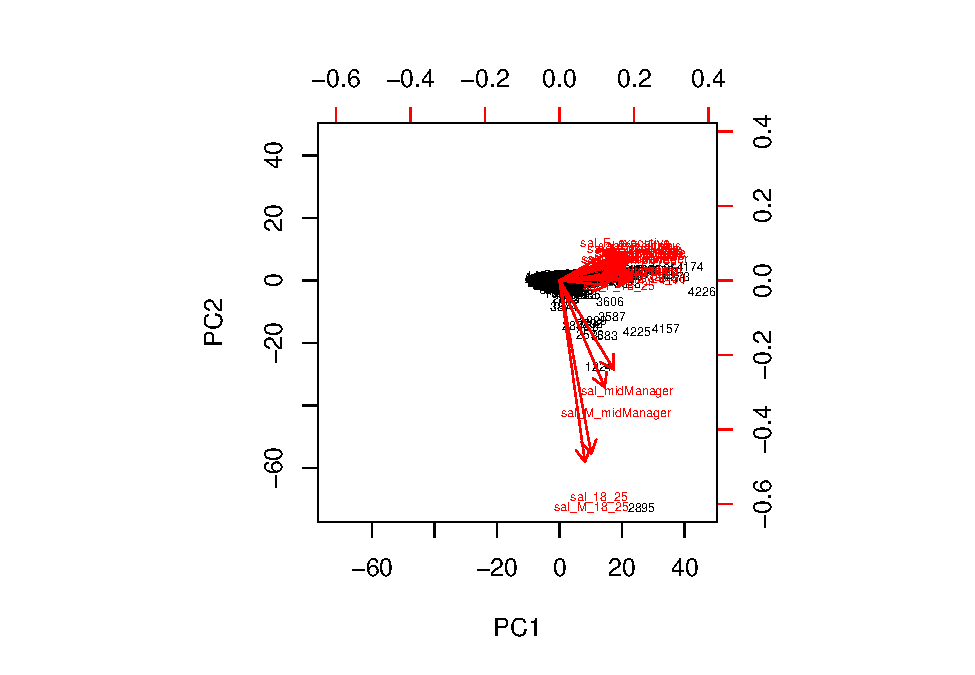
\includegraphics{TSLproject_files/figure-latex/unnamed-chunk-19-2.pdf}

\begin{Shaded}
\begin{Highlighting}[]
\KeywordTok{str}\NormalTok{(myPr)}
\end{Highlighting}
\end{Shaded}

\begin{verbatim}
## List of 5
##  $ sdev    : num [1:24] 4.068 1.43 1.057 1.012 0.883 ...
##  $ rotation: num [1:24, 1:24] 0.243 0.204 0.182 0.224 0.204 ...
##   ..- attr(*, "dimnames")=List of 2
##   .. ..$ : chr [1:24] "sal_general" "sal_executive" "sal_midManager" "sal_employee" ...
##   .. ..$ : chr [1:24] "PC1" "PC2" "PC3" "PC4" ...
##  $ center  : Named num [1:24] 13.7 23.7 14.6 10.6 11.2 ...
##   ..- attr(*, "names")= chr [1:24] "sal_general" "sal_executive" "sal_midManager" "sal_employee" ...
##  $ scale   : Named num [1:24] 2.559 2.836 1.49 0.812 1.222 ...
##   ..- attr(*, "names")= chr [1:24] "sal_general" "sal_executive" "sal_midManager" "sal_employee" ...
##  $ x       : num [1:5136, 1:24] 0.315 -0.185 0.443 -0.74 -0.922 ...
##   ..- attr(*, "dimnames")=List of 2
##   .. ..$ : NULL
##   .. ..$ : chr [1:24] "PC1" "PC2" "PC3" "PC4" ...
##  - attr(*, "class")= chr "prcomp"
\end{verbatim}

\begin{Shaded}
\begin{Highlighting}[]
\CommentTok{#myPr$x #checking principal component scores}
\NormalTok{salary2 <-}\StringTok{ }\KeywordTok{cbind}\NormalTok{(salary, myPr}\OperatorTok{$}\NormalTok{x[, }\DecValTok{1}\OperatorTok{:}\DecValTok{2}\NormalTok{])}
\KeywordTok{head}\NormalTok{(salary2)}
\end{Highlighting}
\end{Shaded}

\begin{verbatim}
##   CODGEO              town sal_general sal_executive sal_midManager
## 1   1004 Ambérieu-en-Bugey        13.7          24.2           15.5
## 2   1007          Ambronay        13.5          22.1           14.7
## 3   1014            Arbent        13.5          27.6           15.6
## 4   1024          Attignat        12.9          21.8           14.1
## 5   1025     Bâgé-la-Ville        13.0          22.8           14.1
## 6   1027             Balan        13.9          22.2           15.1
##   sal_employee sal_worker sal_Females sal_F_executive sal_F_midManager
## 1         10.3       11.2        11.6            19.1             13.2
## 2         10.7       11.4        11.9            19.0             13.3
## 3         11.1       11.1        10.9            19.5             11.7
## 4         11.0       11.3        11.4            19.0             13.0
## 5         10.5       11.1        11.6            19.4             13.6
## 6         11.0       11.4        12.5            20.3             14.0
##   sal_F_employee sal_F_worker sal_Males sal_M_executive sal_M_midManager
## 1           10.1          9.6      15.0            26.4             16.7
## 2           10.6         10.0      14.7            23.3             15.8
## 3           10.8          9.5      15.3            30.2             17.2
## 4           10.3          9.9      13.8            23.0             14.7
## 5           10.2          9.8      13.8            24.1             14.4
## 6           10.9         10.5      15.2            23.1             15.9
##   sal_M_employee sal_M_worker sal_18_25 sal_26_50 sal_51plus sal_F_18_25
## 1           11.0         11.6      10.5      13.7       16.1         9.7
## 2           11.3         11.7       9.8      13.8       14.6         9.2
## 3           12.4         11.8       9.3      13.3       16.0         8.9
## 4           13.2         11.6       9.6      12.9       14.2         9.3
## 5           11.7         11.4       9.4      12.8       15.2         9.0
## 6           12.1         11.7       9.7      14.1       15.4         9.5
##   sal_F_26_50 sal_F_51plus sal_M_18_25 sal_M_26_50 sal_M_51plus        PC1
## 1        11.8         12.5        11.0        14.9         18.6  0.3154969
## 2        12.2         12.5        10.2        14.9         16.4 -0.1853773
## 3        10.6         12.5         9.6        15.1         18.6  0.4431224
## 4        11.4         12.2         9.7        13.8         15.9 -0.7404781
## 5        11.8         12.3         9.7        13.4         16.9 -0.9218165
## 6        12.8         13.0         9.9        15.3         17.2  1.0063385
##           PC2
## 1 -1.51556989
## 2 -0.52833502
## 3 -0.07994227
## 4  0.01522957
## 5  0.22224766
## 6 -0.14256519
\end{verbatim}

\begin{Shaded}
\begin{Highlighting}[]
\CommentTok{#plot with ggplot...}
\CommentTok{#require(ggplot2)}
\KeywordTok{ggplot}\NormalTok{(salary2, }\KeywordTok{aes}\NormalTok{(PC1, PC2)) }\OperatorTok{+}\StringTok{ }
\StringTok{  }\KeywordTok{stat_ellipse}\NormalTok{(}\DataTypeTok{geom =} \StringTok{"polygon"}\NormalTok{, }\DataTypeTok{col =} \StringTok{"black"}\NormalTok{, }\DataTypeTok{alpha =} \FloatTok{0.5}\NormalTok{) }\OperatorTok{+}\StringTok{ }
\StringTok{  }\KeywordTok{geom_point}\NormalTok{(}\DataTypeTok{shape =} \DecValTok{21}\NormalTok{, }\DataTypeTok{col =} \StringTok{"black"}\NormalTok{)}
\end{Highlighting}
\end{Shaded}

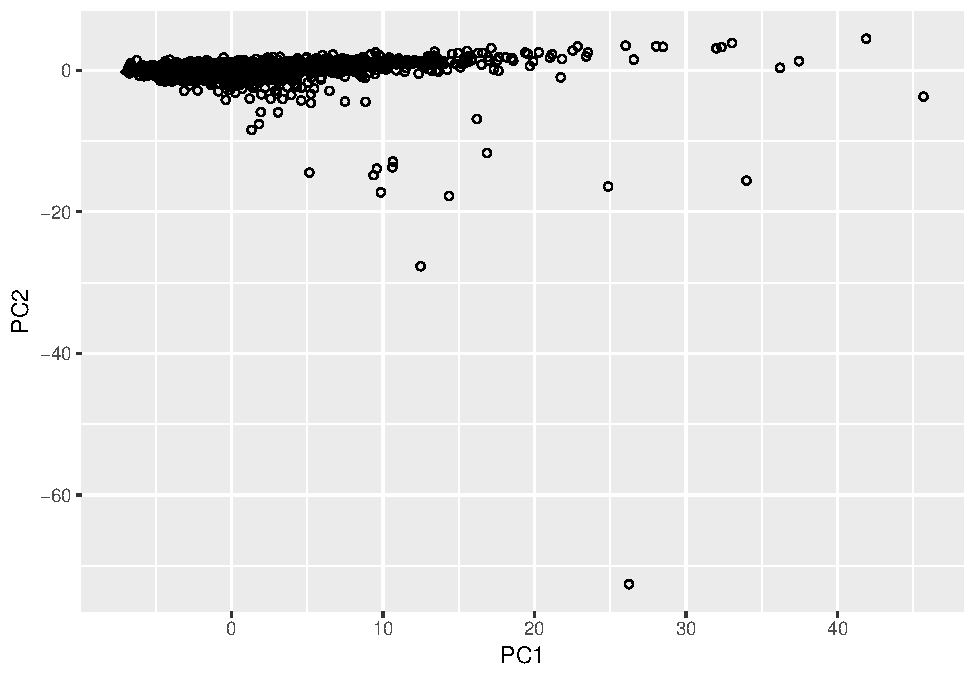
\includegraphics{TSLproject_files/figure-latex/unnamed-chunk-19-3.pdf}

\begin{Shaded}
\begin{Highlighting}[]
\CommentTok{# correlations between variables and PCs...}
\KeywordTok{cor}\NormalTok{(salary[, }\DecValTok{3}\OperatorTok{:}\DecValTok{26}\NormalTok{], salary2[,}\DecValTok{27}\OperatorTok{:}\DecValTok{28}\NormalTok{])}
\end{Highlighting}
\end{Shaded}

\begin{verbatim}
##                        PC1          PC2
## sal_general      0.9868518  0.036371885
## sal_executive    0.8317040  0.129887244
## sal_midManager   0.7400745 -0.426868150
## sal_employee     0.9122603  0.101625280
## sal_worker       0.8284796  0.036732621
## sal_Females      0.9632267  0.110700902
## sal_F_executive  0.7141016  0.143272680
## sal_F_midManager 0.8200819  0.079000080
## sal_F_employee   0.8822511  0.101174610
## sal_F_worker     0.7207812  0.082455908
## sal_Males        0.9754141  0.012951726
## sal_M_executive  0.8051754  0.119379642
## sal_M_midManager 0.6160662 -0.512375927
## sal_M_employee   0.7689048  0.076290041
## sal_M_worker     0.8038938  0.029372055
## sal_18_25        0.4321833 -0.831007140
## sal_26_50        0.9794877  0.031089772
## sal_51plus       0.9631738  0.096273763
## sal_F_18_25      0.6457820 -0.023706420
## sal_F_26_50      0.9546442  0.100680982
## sal_F_51plus     0.9216375  0.127347143
## sal_M_18_25      0.3463258 -0.869883156
## sal_M_26_50      0.9670347  0.004712847
## sal_M_51plus     0.9427597  0.090754879
\end{verbatim}

\subsection{What we have learned}\label{what-we-have-learned-2}

\begin{itemize}
\tightlist
\item
  Check the outlier in sal\_18\_25: which city is it, etc.
\item
  evaluate possible multicollinearity
\item
  Try a regression with all predictors ans lasso
\end{itemize}

\subsection{How to use these data}\label{how-to-use-these-data-2}

\begin{itemize}
\tightlist
\item
  \ldots{}
\end{itemize}

\section{Analyze population data}\label{analyze-population-data}

\subsection{Pre-processing}\label{pre-processing-3}

\begin{Shaded}
\begin{Highlighting}[]
\CommentTok{# preliminary checks}
\KeywordTok{names}\NormalTok{(population)}
\end{Highlighting}
\end{Shaded}

\begin{verbatim}
## [1] "NIVGEO"         "CODGEO"         "LIBGEO"         "MOCO"          
## [5] "ageCateg5"      "sex"            "peopleCategNum"
\end{verbatim}

\begin{Shaded}
\begin{Highlighting}[]
\KeywordTok{summary}\NormalTok{(population)}
\end{Highlighting}
\end{Shaded}

\begin{verbatim}
##  NIVGEO           CODGEO                     LIBGEO             MOCO      
##  COM:8536584   Length:8536584     Sainte-Colombe:   3094   Min.   :11.00  
##                Class :character   Saint-Sauveur :   2618   1st Qu.:12.00  
##                Mode  :character   Sainte-Marie  :   2618   Median :22.00  
##                                   Beaulieu      :   2380   Mean   :21.71  
##                                   Le Pin        :   2380   3rd Qu.:31.00  
##                                   Saint-Aubin   :   2380   Max.   :32.00  
##                                   (Other)       :8521114                  
##    ageCateg5       sex      peopleCategNum    
##  Min.   : 0   Min.   :1.0   Min.   :    0.00  
##  1st Qu.:20   1st Qu.:1.0   1st Qu.:    0.00  
##  Median :40   Median :1.5   Median :    0.00  
##  Mean   :40   Mean   :1.5   Mean   :    7.45  
##  3rd Qu.:60   3rd Qu.:2.0   3rd Qu.:    3.00  
##  Max.   :80   Max.   :2.0   Max.   :48873.00  
## 
\end{verbatim}

\begin{Shaded}
\begin{Highlighting}[]
\CommentTok{# Drop unnecessary columns (NIVGEO is the same for all)}
\NormalTok{population <-}\StringTok{ }\KeywordTok{subset}\NormalTok{(population, }\DataTypeTok{select =} \OperatorTok{-}\KeywordTok{c}\NormalTok{(NIVGEO, LIBGEO))}

\CommentTok{# converting CODGEO to numeric}
\NormalTok{population}\OperatorTok{$}\NormalTok{CODGEO <-}\StringTok{ }\KeywordTok{as.numeric}\NormalTok{(population}\OperatorTok{$}\NormalTok{CODGEO)}

\CommentTok{# Refactor sex and MOCO}
\NormalTok{population}\OperatorTok{$}\NormalTok{MOCO <-}\StringTok{ }\KeywordTok{factor}\NormalTok{(population}\OperatorTok{$}\NormalTok{MOCO, }\DataTypeTok{levels =} \KeywordTok{c}\NormalTok{(}\DecValTok{11}\NormalTok{,}\DecValTok{12}\NormalTok{,}\DecValTok{21}\NormalTok{,}\DecValTok{22}\NormalTok{,}\DecValTok{23}\NormalTok{,}\DecValTok{31}\NormalTok{,}\DecValTok{32}\NormalTok{),}
                          \DataTypeTok{labels =} \KeywordTok{c}\NormalTok{(}\StringTok{"children_living_with_two_parents"}\NormalTok{, }\StringTok{"children living with one parent"}\NormalTok{,}
                                     \StringTok{"adults_living_in_couple_without_child"}\NormalTok{, }\StringTok{"adults_living_in_couple_with_children"}\NormalTok{,}
                                     \StringTok{"adults_living_alone_with_children"}\NormalTok{,}\StringTok{"persons not from family living in the home"}\NormalTok{,}
                                     \StringTok{"persons_living_alone"}\NormalTok{))}
\NormalTok{population}\OperatorTok{$}\NormalTok{sex <-}\StringTok{ }\KeywordTok{factor}\NormalTok{(population}\OperatorTok{$}\NormalTok{sex, }\DataTypeTok{levels =} \KeywordTok{c}\NormalTok{(}\DecValTok{1}\NormalTok{,}\DecValTok{2}\NormalTok{), }\DataTypeTok{labels =} \KeywordTok{c}\NormalTok{(}\StringTok{"Male"}\NormalTok{, }\StringTok{"Female"}\NormalTok{))}
\KeywordTok{head}\NormalTok{(population)}
\end{Highlighting}
\end{Shaded}

\begin{verbatim}
##   CODGEO                             MOCO ageCateg5    sex peopleCategNum
## 1   1001 children_living_with_two_parents         0   Male             15
## 2   1001 children_living_with_two_parents         0 Female             15
## 3   1001 children_living_with_two_parents         5   Male             20
## 4   1001 children_living_with_two_parents         5 Female             20
## 5   1001 children_living_with_two_parents        10   Male             20
## 6   1001 children_living_with_two_parents        10 Female             45
\end{verbatim}

\begin{Shaded}
\begin{Highlighting}[]
\CommentTok{# Take out rows with NB (number of people in this category) equal to 0}
\NormalTok{population <-}\StringTok{ }\NormalTok{population[population}\OperatorTok{$}\NormalTok{peopleCategNum }\OperatorTok{!=}\StringTok{ }\DecValTok{0}\NormalTok{,]}

\KeywordTok{head}\NormalTok{(population)}
\end{Highlighting}
\end{Shaded}

\begin{verbatim}
##   CODGEO                             MOCO ageCateg5    sex peopleCategNum
## 1   1001 children_living_with_two_parents         0   Male             15
## 2   1001 children_living_with_two_parents         0 Female             15
## 3   1001 children_living_with_two_parents         5   Male             20
## 4   1001 children_living_with_two_parents         5 Female             20
## 5   1001 children_living_with_two_parents        10   Male             20
## 6   1001 children_living_with_two_parents        10 Female             45
\end{verbatim}

\begin{Shaded}
\begin{Highlighting}[]
\KeywordTok{summary}\NormalTok{(population)}
\end{Highlighting}
\end{Shaded}

\begin{verbatim}
##      CODGEO                                              MOCO       
##  Min.   : 1001   children_living_with_two_parents          :337182  
##  1st Qu.:27181   children living with one parent           :192130  
##  Median :50394   adults_living_in_couple_without_child     :529268  
##  Mean   :48360   adults_living_in_couple_with_children     :451501  
##  3rd Qu.:69154   adults_living_alone_with_children         :160976  
##  Max.   :97424   persons not from family living in the home:178635  
##                  persons_living_alone                      :361261  
##    ageCateg5         sex          peopleCategNum    
##  Min.   : 0.00   Male  :1106500   Min.   :    1.00  
##  1st Qu.:25.00   Female:1104453   1st Qu.:    4.00  
##  Median :45.00                    Median :    8.00  
##  Mean   :41.77                    Mean   :   28.75  
##  3rd Qu.:60.00                    3rd Qu.:   20.00  
##  Max.   :80.00                    Max.   :48873.00  
## 
\end{verbatim}

\subsection{EDA}\label{eda-3}

\begin{Shaded}
\begin{Highlighting}[]
\CommentTok{#Compare age categories:}
\KeywordTok{library}\NormalTok{(ggplot2)}
\CommentTok{#  number of units}
\NormalTok{n_cat <-}\StringTok{ }\KeywordTok{length}\NormalTok{(population}\OperatorTok{$}\NormalTok{CODGEO)}
\CommentTok{# extract unique categories}
\NormalTok{uniq_cat <-}\StringTok{ }\KeywordTok{unique}\NormalTok{(population}\OperatorTok{$}\NormalTok{ageCateg5}\OperatorTok{!=}\DecValTok{5}\NormalTok{)}
\CommentTok{# vector representing sex for each category}
\NormalTok{Label <-}\StringTok{ }\KeywordTok{c}\NormalTok{(}\KeywordTok{rep}\NormalTok{(}\KeywordTok{c}\NormalTok{(}\StringTok{'Male'}\NormalTok{, }\StringTok{'Female'}\NormalTok{), n_cat))}
\CommentTok{# vector representing the variable considered}
\NormalTok{Variable <-}\StringTok{ }\KeywordTok{rep}\NormalTok{(uniq_cat, n_cat}\OperatorTok{/}\KeywordTok{length}\NormalTok{(uniq_cat))}
\NormalTok{Value=population}\OperatorTok{$}\NormalTok{peopleCategNum}
\CommentTok{# merge these data}
\CommentTok{#pop_categ = cbind.data.frame(Label = Label, }
\CommentTok{#             value = Value,}
\CommentTok{#             Variable = Variable)}
\CommentTok{#p <- ggplot(data = pop_categ, aes(x=Label, y=value)) }
\CommentTok{#p <- p + geom_boxplot(aes(fill = Label))}
\CommentTok{# if you want color for points replace group with colour=Label}
\CommentTok{#p <- p + geom_point(aes(y=value, colour=Label), position = position_dodge(width=0.75))}
\CommentTok{#p <- p + facet_wrap( ~ Variable, scales="free")}
\CommentTok{#p <- p + xlab("x-axis") + ylab("y-axis") + ggtitle("Category comparison")}
\CommentTok{# p <- p + guides(fill=guide_legend(title="Legend"))}
\CommentTok{#p}
\end{Highlighting}
\end{Shaded}

\begin{Shaded}
\begin{Highlighting}[]
\CommentTok{# Restructure population data to produce the demographic profile per town}
\CommentTok{# install.packages("plyr")}
\KeywordTok{library}\NormalTok{(plyr)}
\NormalTok{population_per_town_data <-}\StringTok{ }\KeywordTok{ddply}\NormalTok{(population, .(CODGEO), }\ControlFlowTok{function}\NormalTok{(population) \{}
  \KeywordTok{data.frame}\NormalTok{(}\DataTypeTok{total_population =} \KeywordTok{sum}\NormalTok{(population}\OperatorTok{$}\NormalTok{peopleCategNum),}
             \DataTypeTok{male =} \KeywordTok{sum}\NormalTok{(population[population}\OperatorTok{$}\NormalTok{sex }\OperatorTok{==}\StringTok{ "Male"}\NormalTok{,]}\OperatorTok{$}\NormalTok{peopleCategNum),}
             \DataTypeTok{female =} \KeywordTok{sum}\NormalTok{(population[population}\OperatorTok{$}\NormalTok{sex }\OperatorTok{==}\StringTok{ "Female"}\NormalTok{,]}\OperatorTok{$}\NormalTok{peopleCategNum),}
             \DataTypeTok{child =} \KeywordTok{sum}\NormalTok{(population[population}\OperatorTok{$}\NormalTok{ageCateg5 }\OperatorTok\StringTok{ }\KeywordTok{seq}\NormalTok{(}\DecValTok{0}\NormalTok{, }\DecValTok{10}\NormalTok{, }\DataTypeTok{by=}\DecValTok{5}\NormalTok{),]}\OperatorTok{$}\NormalTok{peopleCategNum),}
             \DataTypeTok{elderly =} \KeywordTok{sum}\NormalTok{(population[population}\OperatorTok{$}\NormalTok{ageCateg5 }\OperatorTok\StringTok{ }\KeywordTok{seq}\NormalTok{(}\DecValTok{65}\NormalTok{, }\DecValTok{80}\NormalTok{, }\DataTypeTok{by=}\DecValTok{5}\NormalTok{),]}\OperatorTok{$}\NormalTok{peopleCategNum),}
             \DataTypeTok{workforce =} \KeywordTok{sum}\NormalTok{(population[population}\OperatorTok{$}\NormalTok{ageCateg5 }\OperatorTok\StringTok{ }\KeywordTok{seq}\NormalTok{(}\DecValTok{15}\NormalTok{, }\DecValTok{60}\NormalTok{, }\DataTypeTok{by=}\DecValTok{5}\NormalTok{),]}\OperatorTok{$}\NormalTok{peopleCategNum) }
\NormalTok{  )\})}

\NormalTok{population_per_town_data}\OperatorTok{$}\NormalTok{dependent <-}\StringTok{ }\NormalTok{population_per_town_data}\OperatorTok{$}\NormalTok{child }\OperatorTok{+}\StringTok{ }\NormalTok{population_per_town_data}\OperatorTok{$}\NormalTok{elderly}
\NormalTok{population_per_town_data}\OperatorTok{$}\NormalTok{sex_ratio <-}\StringTok{ }\KeywordTok{ifelse}\NormalTok{(population_per_town_data}\OperatorTok{$}\NormalTok{female}\OperatorTok{==}\DecValTok{0}\NormalTok{, }\DecValTok{0}\NormalTok{, population_per_town_data}\OperatorTok{$}\NormalTok{male }\OperatorTok{/}\StringTok{ }\NormalTok{population_per_town_data}\OperatorTok{$}\NormalTok{female)}
\NormalTok{population_per_town_data}\OperatorTok{$}\NormalTok{dependency_ratio <-}\StringTok{ }\KeywordTok{ifelse}\NormalTok{(population_per_town_data}\OperatorTok{$}\NormalTok{workforce}\OperatorTok{==}\DecValTok{0}\NormalTok{, }\DecValTok{0}\NormalTok{, population_per_town_data}\OperatorTok{$}\NormalTok{dependent }\OperatorTok{/}\StringTok{ }\NormalTok{population_per_town_data}\OperatorTok{$}\NormalTok{workforce)}
\NormalTok{population_per_town_data}\OperatorTok{$}\NormalTok{aged_dependency_ratio <-}\StringTok{ }\KeywordTok{ifelse}\NormalTok{(population_per_town_data}\OperatorTok{$}\NormalTok{workforce}\OperatorTok{==}\DecValTok{0}\NormalTok{, }\DecValTok{0}\NormalTok{, population_per_town_data}\OperatorTok{$}\NormalTok{elderly }\OperatorTok{/}\StringTok{ }\NormalTok{population_per_town_data}\OperatorTok{$}\NormalTok{workforce)}
\NormalTok{population_per_town_data}\OperatorTok{$}\NormalTok{child_dependency_ratio <-}\StringTok{ }\KeywordTok{ifelse}\NormalTok{(population_per_town_data}\OperatorTok{$}\NormalTok{workforce}\OperatorTok{==}\DecValTok{0}\NormalTok{, }\DecValTok{0}\NormalTok{, population_per_town_data}\OperatorTok{$}\NormalTok{child }\OperatorTok{/}\StringTok{ }\NormalTok{population_per_town_data}\OperatorTok{$}\NormalTok{workforce)}
\KeywordTok{summary}\NormalTok{(population_per_town_data)}
\end{Highlighting}
\end{Shaded}

\begin{verbatim}
##      CODGEO      total_population       male               female         
##  Min.   : 1001   Min.   :      2   Min.   :      0.0   Min.   :      0.0  
##  1st Qu.:24541   1st Qu.:    184   1st Qu.:     92.0   1st Qu.:     90.0  
##  Median :48098   Median :    420   Median :    212.0   Median :    209.0  
##  Mean   :46276   Mean   :   1773   Mean   :    857.6   Mean   :    915.4  
##  3rd Qu.:67076   3rd Qu.:   1060   3rd Qu.:    528.0   3rd Qu.:    535.0  
##  Max.   :97424   Max.   :2173279   Max.   :1018597.0   Max.   :1154682.0  
##      child             elderly           workforce        
##  Min.   :     0.0   Min.   :     0.0   Min.   :      0.0  
##  1st Qu.:    32.0   1st Qu.:    35.0   1st Qu.:    112.0  
##  Median :    80.0   Median :    75.0   Median :    261.0  
##  Mean   :   333.9   Mean   :   310.1   Mean   :   1128.9  
##  3rd Qu.:   209.5   3rd Qu.:   190.0   3rd Qu.:    659.5  
##  Max.   :315127.0   Max.   :338074.0   Max.   :1520078.0  
##    dependent          sex_ratio       dependency_ratio
##  Min.   :     0.0   Min.   : 0.0000   Min.   :0.0000  
##  1st Qu.:    70.0   1st Qu.: 0.9075   1st Qu.:0.5135  
##  Median :   160.0   Median : 0.9971   Median :0.6088  
##  Mean   :   644.1   Mean   : 1.0259   Mean   :0.6538  
##  3rd Qu.:   401.0   3rd Qu.: 1.1026   3rd Qu.:0.7333  
##  Max.   :653201.0   Max.   :10.0000   Max.   :9.0000  
##  aged_dependency_ratio child_dependency_ratio
##  Min.   :0.0000        Min.   :0.0000        
##  1st Qu.:0.2091        1st Qu.:0.2453        
##  Median :0.2929        Median :0.3043        
##  Mean   :0.3462        Mean   :0.3076        
##  3rd Qu.:0.4166        3rd Qu.:0.3662        
##  Max.   :8.0000        Max.   :3.0000
\end{verbatim}

\begin{Shaded}
\begin{Highlighting}[]
\CommentTok{# Scale population to log}
\KeywordTok{hist}\NormalTok{(population_per_town_data}\OperatorTok{$}\NormalTok{total_population, }\DataTypeTok{ylim=}\KeywordTok{c}\NormalTok{(}\DecValTok{0}\NormalTok{,}\DecValTok{40000}\NormalTok{), }\DataTypeTok{breaks =} \KeywordTok{seq}\NormalTok{(}\DecValTok{0}\NormalTok{, }\DecValTok{2500000}\NormalTok{, }\DataTypeTok{by=}\DecValTok{250000}\NormalTok{), }\DataTypeTok{xlab=}\StringTok{""}\NormalTok{, }\DataTypeTok{main =} \StringTok{""}\NormalTok{, }\DataTypeTok{labels=}\NormalTok{T, }\DataTypeTok{col =}\StringTok{"light blue"}\NormalTok{)}
\end{Highlighting}
\end{Shaded}

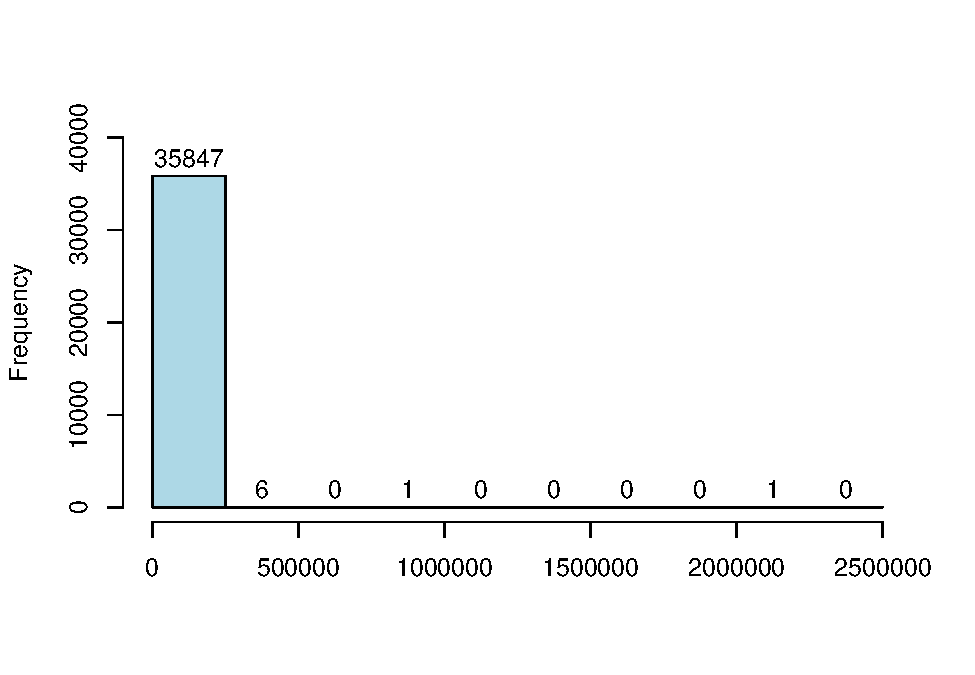
\includegraphics{TSLproject_files/figure-latex/unnamed-chunk-23-1.pdf}

\begin{Shaded}
\begin{Highlighting}[]
\NormalTok{population_per_town_data}\OperatorTok{$}\NormalTok{total_population_log <-}\StringTok{ }\KeywordTok{log10}\NormalTok{(population_per_town_data}\OperatorTok{$}\NormalTok{total_population)}

\CommentTok{# Merge geo and pop}
\NormalTok{geo_pop_by_town <-}\StringTok{ }\KeywordTok{merge}\NormalTok{(geo, population_per_town_data)}
\KeywordTok{summary}\NormalTok{(geo_pop_by_town)}
\end{Highlighting}
\end{Shaded}

\begin{verbatim}
##      CODGEO                region       region_capital 
##  Min.   : 1001   Midi-Pyrénées: 2980   Toulouse: 2980  
##  1st Qu.:24510   Rhône-Alpes  : 2835   Lyon    : 2835  
##  Median :48044   Lorraine     : 2323   Metz    : 2323  
##  Mean   :46129   Aquitaine    : 2282   Bordeaux: 2282  
##  3rd Qu.:67004   Picardie     : 2277   Amiens  : 2277  
##  Max.   :97126   Bourgogne    : 2018   Dijon   : 2018  
##                  (Other)      :21046   (Other) :21046  
##           department             town_name      postal_code   
##  Pas-de-Calais :  892   Paris         :   19   51300  :   46  
##  Aisne         :  805   Sainte-Colombe:   14   51800  :   44  
##  Somme         :  782   Saint-Sauveur :   12   70000  :   42  
##  Moselle       :  729   Beaulieu      :   10   88500  :   42  
##  Seine-Maritime:  718   Beaumont      :   10   80140  :   40  
##  Côte-d'Or     :  705   Saint-Aubin   :   10   10200  :   36  
##  (Other)       :31130   (Other)       :35686   (Other):35511  
##     latitude       longitude       total_population       male        
##  Min.   :41.39   Min.   :-5.0914   Min.   :      2   Min.   :      0  
##  1st Qu.:45.13   1st Qu.: 0.7333   1st Qu.:    184   1st Qu.:     92  
##  Median :47.37   Median : 2.6833   Median :    420   Median :    210  
##  Mean   :46.96   Mean   : 2.7747   Mean   :   3024   Mean   :   1444  
##  3rd Qu.:48.83   3rd Qu.: 4.8833   3rd Qu.:   1054   3rd Qu.:    524  
##  Max.   :51.08   Max.   : 9.5167   Max.   :2173279   Max.   :1018597  
##                                                                       
##      female            child             elderly         workforce      
##  Min.   :      0   Min.   :     0.0   Min.   :     0   Min.   :      0  
##  1st Qu.:     90   1st Qu.:    32.0   1st Qu.:    35   1st Qu.:    112  
##  Median :    208   Median :    80.0   Median :    75   Median :    260  
##  Mean   :   1580   Mean   :   518.2   Mean   :   510   Mean   :   1996  
##  3rd Qu.:    530   3rd Qu.:   208.0   3rd Qu.:   190   3rd Qu.:    655  
##  Max.   :1154682   Max.   :315127.0   Max.   :338074   Max.   :1520078  
##                                                                         
##    dependent        sex_ratio       dependency_ratio aged_dependency_ratio
##  Min.   :     0   Min.   : 0.0000   Min.   :0.0000   Min.   :0.0000       
##  1st Qu.:    70   1st Qu.: 0.9074   1st Qu.:0.5132   1st Qu.:0.2094       
##  Median :   160   Median : 0.9974   Median :0.6090   Median :0.2932       
##  Mean   :  1028   Mean   : 1.0259   Mean   :0.6539   Mean   :0.3465       
##  3rd Qu.:   399   3rd Qu.: 1.1029   3rd Qu.:0.7333   3rd Qu.:0.4167       
##  Max.   :653201   Max.   :10.0000   Max.   :9.0000   Max.   :8.0000       
##                                                                           
##  child_dependency_ratio total_population_log
##  Min.   :0.0000         Min.   :0.301       
##  1st Qu.:0.2450         1st Qu.:2.265       
##  Median :0.3043         Median :2.623       
##  Mean   :0.3073         Mean   :2.674       
##  3rd Qu.:0.3661         3rd Qu.:3.023       
##  Max.   :3.0000         Max.   :6.337       
## 
\end{verbatim}

\begin{Shaded}
\begin{Highlighting}[]
\CommentTok{# Plot "Distribution of Population for each Town"}
\CommentTok{#myPalette(low = "white", high = c("green", "red"), mid=NULL, k =50)-Need "GLAD" package}
\NormalTok{sc <-}\StringTok{ }\KeywordTok{scale_colour_gradientn}\NormalTok{(}\DataTypeTok{colours =}\KeywordTok{palette}\NormalTok{(}\KeywordTok{rainbow}\NormalTok{(}\DecValTok{8}\NormalTok{)), }\DataTypeTok{limits=}\KeywordTok{c}\NormalTok{(}\KeywordTok{min}\NormalTok{(geo_pop_by_town}\OperatorTok{$}\NormalTok{total_population_log), }\KeywordTok{max}\NormalTok{(geo_pop_by_town}\OperatorTok{$}\NormalTok{total_population_log)))}
\NormalTok{poppulation_distribution <-}\StringTok{ }
\StringTok{  }\NormalTok{FraMap }\OperatorTok{+}\StringTok{ }
\StringTok{  }\KeywordTok{geom_point}\NormalTok{(}\KeywordTok{aes}\NormalTok{(}\DataTypeTok{x=}\NormalTok{geo_pop_by_town}\OperatorTok{$}\NormalTok{longitude, }\DataTypeTok{y=}\NormalTok{geo_pop_by_town}\OperatorTok{$}\NormalTok{latitude, }\DataTypeTok{colour=}\NormalTok{geo_pop_by_town}\OperatorTok{$}\NormalTok{total_population_log), }
             \DataTypeTok{data=}\NormalTok{geo_pop_by_town, }\DataTypeTok{alpha=}\FloatTok{0.8}\NormalTok{, }\DataTypeTok{size=}\FloatTok{0.6}\NormalTok{) }\OperatorTok{+}\StringTok{ }
\StringTok{  }\NormalTok{sc }\OperatorTok{+}
\StringTok{  }\KeywordTok{geom_text}\NormalTok{(}\KeywordTok{aes}\NormalTok{(}\DataTypeTok{label =}\NormalTok{ town_name, }\DataTypeTok{x =}\NormalTok{ longitude, }\DataTypeTok{y =}\NormalTok{ latitude), }
            \DataTypeTok{data =} \KeywordTok{subset}\NormalTok{(geo_pop_by_town, total_population_log }\OperatorTok\StringTok{ }\KeywordTok{head}\NormalTok{(}\KeywordTok{sort}\NormalTok{(total_population_log, }\DataTypeTok{decreasing=}\OtherTok{TRUE}\NormalTok{), }\DecValTok{3}\NormalTok{)),}
            \DataTypeTok{check_overlap =} \OtherTok{TRUE}\NormalTok{, }\DataTypeTok{size=}\DecValTok{7}\NormalTok{) }\OperatorTok{+}
\StringTok{  }\KeywordTok{labs}\NormalTok{(}\DataTypeTok{color=}\StringTok{'Total Population in Log'}\NormalTok{) }\OperatorTok{+}
\StringTok{  }\KeywordTok{ggtitle}\NormalTok{(}\StringTok{"Distribution of Population for each Town"}\NormalTok{) }
\NormalTok{poppulation_distribution}
\end{Highlighting}
\end{Shaded}

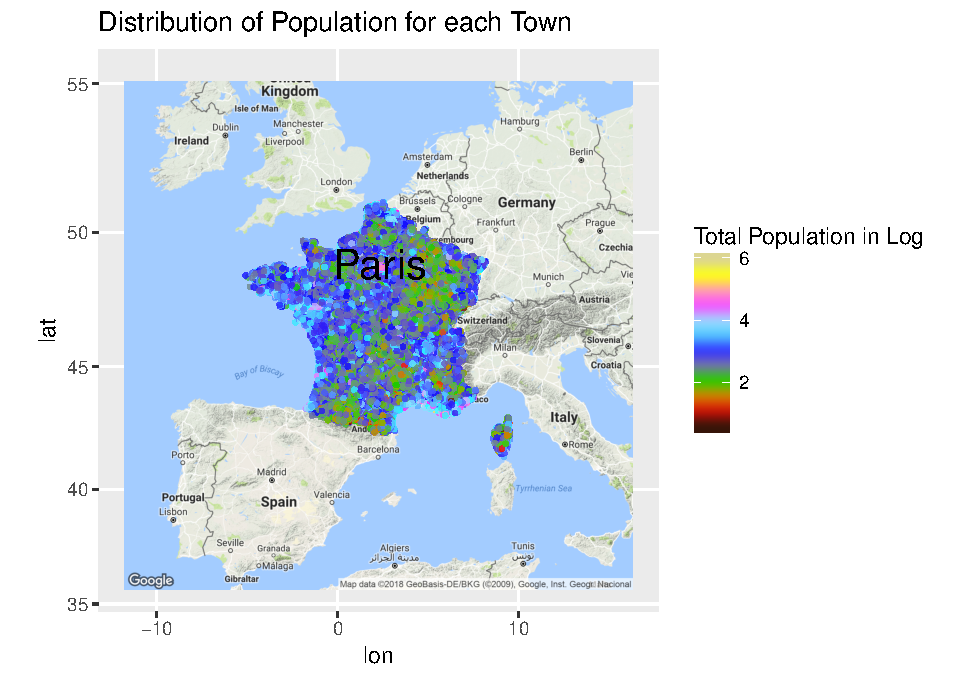
\includegraphics{TSLproject_files/figure-latex/unnamed-chunk-23-2.pdf}

\begin{Shaded}
\begin{Highlighting}[]
\CommentTok{# Group population data by department because of small size of some towns and the given geojson file of department}
\NormalTok{pop_by_department <-}\StringTok{ }\KeywordTok{ddply}\NormalTok{(geo_pop_by_town, .(department), }\ControlFlowTok{function}\NormalTok{(geo_pop_by_town) \{}
  \KeywordTok{data.frame}\NormalTok{(}\DataTypeTok{total_population =} \KeywordTok{sum}\NormalTok{(geo_pop_by_town}\OperatorTok{$}\NormalTok{total_population),}
             \DataTypeTok{male =} \KeywordTok{sum}\NormalTok{(geo_pop_by_town}\OperatorTok{$}\NormalTok{male),}
             \DataTypeTok{female =} \KeywordTok{sum}\NormalTok{(geo_pop_by_town}\OperatorTok{$}\NormalTok{female),}
             \DataTypeTok{child =} \KeywordTok{sum}\NormalTok{(geo_pop_by_town}\OperatorTok{$}\NormalTok{child),}
             \DataTypeTok{elderly =} \KeywordTok{sum}\NormalTok{(geo_pop_by_town}\OperatorTok{$}\NormalTok{elderly),}
             \DataTypeTok{dependent =} \KeywordTok{sum}\NormalTok{(geo_pop_by_town}\OperatorTok{$}\NormalTok{dependent),}
             \DataTypeTok{workforce =} \KeywordTok{sum}\NormalTok{(geo_pop_by_town}\OperatorTok{$}\NormalTok{workforce) }
\NormalTok{  )\})}

\KeywordTok{summary}\NormalTok{(pop_by_department)}
\end{Highlighting}
\end{Shaded}

\begin{verbatim}
##                    department total_population        male         
##  Ain                    : 1   Min.   :    9048   Min.   :    4353  
##  Aisne                  : 1   1st Qu.:  268814   1st Qu.:  131022  
##  Allier                 : 1   Median :  512671   Median :  250784  
##  Alpes-de-Haute-Provence: 1   Mean   : 1114958   Mean   :  532357  
##  Alpes-Maritimes        : 1   3rd Qu.:  782721   3rd Qu.:  383158  
##  Ardèche                : 1   Max.   :41292301   Max.   :19353343  
##  (Other)                :91                                        
##      female             child            elderly          dependent       
##  Min.   :    4695   Min.   :   1700   Min.   :   2076   Min.   :    3776  
##  1st Qu.:  137792   1st Qu.:  50051   1st Qu.:  55801   1st Qu.:  107317  
##  Median :  261218   Median :  91961   Median :  92779   Median :  187742  
##  Mean   :  582601   Mean   : 191059   Mean   : 188003   Mean   :  379062  
##  3rd Qu.:  399563   3rd Qu.: 156655   3rd Qu.: 146183   3rd Qu.:  287695  
##  Max.   :21938958   Max.   :5987413   Max.   :6423406   Max.   :12410819  
##                                                                           
##    workforce       
##  Min.   :    5272  
##  1st Qu.:  168468  
##  Median :  324657  
##  Mean   :  735896  
##  3rd Qu.:  505345  
##  Max.   :28881482  
## 
\end{verbatim}

\begin{Shaded}
\begin{Highlighting}[]
\NormalTok{pop_by_department}\OperatorTok{$}\NormalTok{dependency_ratio <-}\StringTok{ }\NormalTok{pop_by_department}\OperatorTok{$}\NormalTok{dependent }\OperatorTok{/}\StringTok{ }\NormalTok{pop_by_department}\OperatorTok{$}\NormalTok{workforce}
\NormalTok{pop_by_department}\OperatorTok{$}\NormalTok{aged_dependency_ratio <-}\StringTok{ }\NormalTok{pop_by_department}\OperatorTok{$}\NormalTok{elderly }\OperatorTok{/}\StringTok{ }\NormalTok{pop_by_department}\OperatorTok{$}\NormalTok{workforce}
\NormalTok{pop_by_department}\OperatorTok{$}\NormalTok{child_dependency_ratio <-}\StringTok{ }\NormalTok{pop_by_department}\OperatorTok{$}\NormalTok{child }\OperatorTok{/}\StringTok{ }\NormalTok{pop_by_department}\OperatorTok{$}\NormalTok{workforce}
\end{Highlighting}
\end{Shaded}

\begin{Shaded}
\begin{Highlighting}[]
\CommentTok{# Scale population to log}
\NormalTok{pop_by_department}\OperatorTok{$}\NormalTok{total_population_log <-}\StringTok{ }\KeywordTok{log10}\NormalTok{(pop_by_department}\OperatorTok{$}\NormalTok{total_population)}

\CommentTok{# Merge geo and pop}
\NormalTok{geo_pop_by_department <-}\StringTok{ }\KeywordTok{merge}\NormalTok{(geo, pop_by_department)}
\KeywordTok{summary}\NormalTok{(geo_pop_by_department)}
\end{Highlighting}
\end{Shaded}

\begin{verbatim}
##           department              region       region_capital 
##  Pas-de-Calais :  894   Midi-Pyrénées: 3021   Toulouse: 3021  
##  Aisne         :  816   Rhône-Alpes  : 2882   Lyon    : 2882  
##  Somme         :  782   Lorraine     : 2333   Metz    : 2333  
##  Seine-Maritime:  745   Aquitaine    : 2296   Bordeaux: 2296  
##  Moselle       :  730   Picardie     : 2291   Amiens  : 2291  
##  Côte-d'Or     :  707   Bourgogne    : 2046   Dijon   : 2046  
##  (Other)       :31920   (Other)      :21725   (Other) :21725  
##           town_name      postal_code        CODGEO         latitude    
##  Paris         :   19   51300  :   46   Min.   : 1001   Min.   :41.39  
##  Sainte-Colombe:   14   51800  :   44   1st Qu.:24527   1st Qu.:45.17  
##  Saint-Sauveur :   12   70000  :   42   Median :48111   Median :47.40  
##  Beaulieu      :   11   88500  :   42   Mean   :46096   Mean   :46.98  
##  Saint-Sulpice :   11   80140  :   40   3rd Qu.:66169   3rd Qu.:48.83  
##  Beaumont      :   10   02160  :   38   Max.   :97126   Max.   :51.08  
##  (Other)       :36517   (Other):36342                                  
##    longitude       total_population        male         
##  Min.   :-5.0914   Min.   :    9048   Min.   :    4353  
##  1st Qu.: 0.6667   1st Qu.:  317665   1st Qu.:  153234  
##  Median : 2.6333   Median :  529618   Median :  257449  
##  Mean   : 2.7380   Mean   :  694650   Mean   :  336127  
##  3rd Qu.: 4.8667   3rd Qu.:  776291   3rd Qu.:  378636  
##  Max.   : 9.5167   Max.   :41292301   Max.   :19353343  
##                                                         
##      female             child            elderly          dependent       
##  Min.   :    4695   Min.   :   1700   Min.   :   2076   Min.   :    3776  
##  1st Qu.:  162818   1st Qu.:  54952   1st Qu.:  66927   1st Qu.:  125937  
##  Median :  272169   Median : 101471   Median :  93119   Median :  193520  
##  Mean   :  358523   Mean   : 129285   Mean   : 122310   Mean   :  251595  
##  3rd Qu.:  397655   3rd Qu.: 156655   3rd Qu.: 143873   3rd Qu.:  278973  
##  Max.   :21938958   Max.   :5987413   Max.   :6423406   Max.   :12410819  
##                                                                           
##    workforce        dependency_ratio aged_dependency_ratio
##  Min.   :    5272   Min.   :0.4297   Min.   :0.1636       
##  1st Qu.:  189820   1st Qu.:0.5571   1st Qu.:0.2606       
##  Median :  326192   Median :0.6023   Median :0.3071       
##  Mean   :  443055   Mean   :0.6014   Mean   :0.3101       
##  3rd Qu.:  496202   3rd Qu.:0.6458   3rd Qu.:0.3570       
##  Max.   :28881482   Max.   :0.7162   Max.   :0.4536       
##                                                           
##  child_dependency_ratio total_population_log
##  Min.   :0.2073         Min.   :3.957       
##  1st Qu.:0.2708         1st Qu.:5.502       
##  Median :0.2920         Median :5.724       
##  Mean   :0.2913         Mean   :5.710       
##  3rd Qu.:0.3054         3rd Qu.:5.890       
##  Max.   :0.3468         Max.   :7.616       
## 
\end{verbatim}

\begin{Shaded}
\begin{Highlighting}[]
\CommentTok{# Plot "Distribution of Population for each department"}
\CommentTok{#myPalette(low = "white", high = c("green", "red"), mid=NULL, k =50)-Need "GLAD" package}
\NormalTok{sc <-}\StringTok{ }\KeywordTok{scale_colour_gradientn}\NormalTok{(}\DataTypeTok{colours =}\KeywordTok{palette}\NormalTok{(}\KeywordTok{rainbow}\NormalTok{(}\DecValTok{8}\NormalTok{)), }\DataTypeTok{limits=}\KeywordTok{c}\NormalTok{(}\KeywordTok{min}\NormalTok{(geo_pop_by_department}\OperatorTok{$}\NormalTok{total_population_log), }\KeywordTok{max}\NormalTok{(geo_pop_by_department}\OperatorTok{$}\NormalTok{total_population_log)))}
\NormalTok{pop_distribution_department <-}\StringTok{ }
\StringTok{  }\NormalTok{FraMap }\OperatorTok{+}\StringTok{ }
\StringTok{  }\KeywordTok{geom_point}\NormalTok{(}\KeywordTok{aes}\NormalTok{(}\DataTypeTok{x=}\NormalTok{geo_pop_by_department}\OperatorTok{$}\NormalTok{longitude, }\DataTypeTok{y=}\NormalTok{geo_pop_by_department}\OperatorTok{$}\NormalTok{latitude, }\DataTypeTok{colour=}\NormalTok{geo_pop_by_department}\OperatorTok{$}\NormalTok{total_population_log), }
             \DataTypeTok{data=}\NormalTok{geo_pop_by_department, }\DataTypeTok{alpha=}\FloatTok{0.8}\NormalTok{, }\DataTypeTok{size=}\FloatTok{0.6}\NormalTok{) }\OperatorTok{+}\StringTok{ }
\StringTok{  }\NormalTok{sc }\OperatorTok{+}
\StringTok{  }\KeywordTok{geom_text}\NormalTok{(}\KeywordTok{aes}\NormalTok{(}\DataTypeTok{label =}\NormalTok{ town_name, }\DataTypeTok{x =}\NormalTok{ longitude, }\DataTypeTok{y =}\NormalTok{ latitude), }
            \DataTypeTok{data =} \KeywordTok{subset}\NormalTok{(geo_pop_by_department, total_population_log }\OperatorTok\StringTok{ }\KeywordTok{head}\NormalTok{(}\KeywordTok{sort}\NormalTok{(total_population_log, }\DataTypeTok{decreasing=}\OtherTok{TRUE}\NormalTok{), }\DecValTok{3}\NormalTok{)),}
            \DataTypeTok{check_overlap =} \OtherTok{TRUE}\NormalTok{, }\DataTypeTok{size=}\DecValTok{7}\NormalTok{) }\OperatorTok{+}
\StringTok{  }\KeywordTok{labs}\NormalTok{(}\DataTypeTok{color=}\StringTok{'Total Population in Log'}\NormalTok{) }\OperatorTok{+}
\StringTok{  }\KeywordTok{ggtitle}\NormalTok{(}\StringTok{"Distribution of Population for each department"}\NormalTok{) }
\NormalTok{pop_distribution_department}
\end{Highlighting}
\end{Shaded}

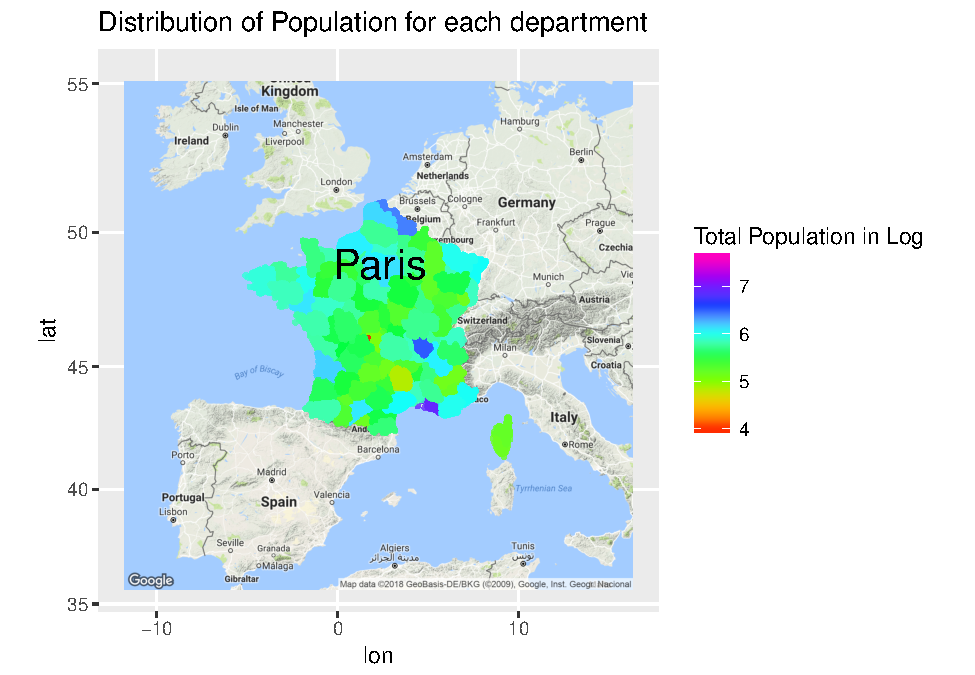
\includegraphics{TSLproject_files/figure-latex/unnamed-chunk-26-1.pdf}

\section{Produce consistent datasets}\label{produce-consistent-datasets}

\begin{Shaded}
\begin{Highlighting}[]
\CommentTok{# use only integer values}
\NormalTok{geo}\OperatorTok{$}\NormalTok{CODGEO =}\StringTok{ }\KeywordTok{as.integer}\NormalTok{(geo}\OperatorTok{$}\NormalTok{CODGEO)  }\CommentTok{# already integer}
\NormalTok{population}\OperatorTok{$}\NormalTok{CODGEO =}\StringTok{ }\KeywordTok{as.integer}\NormalTok{(population}\OperatorTok{$}\NormalTok{CODGEO)}
\NormalTok{firms}\OperatorTok{$}\NormalTok{CODGEO =}\StringTok{ }\KeywordTok{as.integer}\NormalTok{(firms}\OperatorTok{$}\NormalTok{CODGEO)}
\NormalTok{salary}\OperatorTok{$}\NormalTok{CODGEO =}\StringTok{ }\KeywordTok{as.integer}\NormalTok{(salary}\OperatorTok{$}\NormalTok{CODGEO)}

\CommentTok{# install.packages("dplyr")}
\KeywordTok{library}\NormalTok{(dplyr)}
\end{Highlighting}
\end{Shaded}

\begin{verbatim}
## 
## Attaching package: 'dplyr'
\end{verbatim}

\begin{verbatim}
## The following objects are masked from 'package:plyr':
## 
##     arrange, count, desc, failwith, id, mutate, rename, summarise,
##     summarize
\end{verbatim}

\begin{verbatim}
## The following objects are masked from 'package:stats':
## 
##     filter, lag
\end{verbatim}

\begin{verbatim}
## The following objects are masked from 'package:base':
## 
##     intersect, setdiff, setequal, union
\end{verbatim}

\begin{Shaded}
\begin{Highlighting}[]
\NormalTok{dataset =}\StringTok{ }\KeywordTok{c}\NormalTok{(}\StringTok{"population"}\NormalTok{, }\StringTok{"salary"}\NormalTok{, }\StringTok{"firms"}\NormalTok{, }\StringTok{"geo"}\NormalTok{)}

\CommentTok{# obtain sommon IDs for all datasets}
\ControlFlowTok{for}\NormalTok{ (i }\ControlFlowTok{in}\NormalTok{ dataset)\{}
  \CommentTok{# get i-th name and make a new variable adding NEW}
\NormalTok{  nam <-}\StringTok{ }\KeywordTok{paste}\NormalTok{(i, }\StringTok{"NEW"}\NormalTok{, }\DataTypeTok{sep =} \StringTok{""}\NormalTok{)}
  \CommentTok{# counter to identify the number of iteration in j}
\NormalTok{  iter =}\StringTok{ }\DecValTok{1}
  \ControlFlowTok{for}\NormalTok{ (j }\ControlFlowTok{in}\NormalTok{ dataset)\{}
    \ControlFlowTok{if}\NormalTok{ (j }\OperatorTok{!=}\StringTok{ }\NormalTok{i)\{}
      \CommentTok{# datasets different from i-th}
      \ControlFlowTok{if}\NormalTok{ (iter }\OperatorTok{==}\StringTok{ }\DecValTok{1}\NormalTok{)\{}
        \CommentTok{# 1st iteration: use the original dataset (e.g., geo)}
        \KeywordTok{assign}\NormalTok{(nam, }\KeywordTok{semi_join}\NormalTok{(}\KeywordTok{get}\NormalTok{(i), }\KeywordTok{get}\NormalTok{(j), }\DataTypeTok{by =} \StringTok{"CODGEO"}\NormalTok{))}
\NormalTok{      \} }\ControlFlowTok{else}\NormalTok{\{}
        \CommentTok{# successive iteration: use the new dataset (e.g., geoNEW)}
        \KeywordTok{assign}\NormalTok{(nam, }\KeywordTok{semi_join}\NormalTok{(}\KeywordTok{get}\NormalTok{(nam), }\KeywordTok{get}\NormalTok{(j), }\DataTypeTok{by =} \StringTok{"CODGEO"}\NormalTok{))}
\NormalTok{      \}}
\NormalTok{      iter =}\StringTok{ }\NormalTok{iter }\OperatorTok{+}\StringTok{ }\DecValTok{1}
\NormalTok{    \}}
\NormalTok{  \}}
\NormalTok{\}}

\CommentTok{# check how many observation have been deleted}
\ControlFlowTok{for}\NormalTok{ (i }\ControlFlowTok{in}\NormalTok{ dataset)\{}
\NormalTok{  del_rows =}\StringTok{ }\KeywordTok{nrow}\NormalTok{(}\KeywordTok{get}\NormalTok{(i)) }\OperatorTok{-}\StringTok{ }\KeywordTok{nrow}\NormalTok{(}\KeywordTok{get}\NormalTok{(}\KeywordTok{paste}\NormalTok{(i, }\StringTok{"NEW"}\NormalTok{, }\DataTypeTok{sep =} \StringTok{""}\NormalTok{)))}
\NormalTok{  del_prop =}\StringTok{ }\NormalTok{del_rows }\OperatorTok{/}\StringTok{ }\KeywordTok{nrow}\NormalTok{(}\KeywordTok{get}\NormalTok{(}\KeywordTok{paste}\NormalTok{(i, }\StringTok{"NEW"}\NormalTok{, }\DataTypeTok{sep =} \StringTok{""}\NormalTok{)))}
\NormalTok{  del_obs =}\StringTok{ }\KeywordTok{paste}\NormalTok{(}\StringTok{"For"}\NormalTok{, i, del_rows, }\StringTok{"have been deleted."}\NormalTok{,}
                  \StringTok{"They were the"}\NormalTok{, }\KeywordTok{round}\NormalTok{(del_prop, }\DataTypeTok{digits=}\DecValTok{2}\NormalTok{), }\StringTok{"% of the total."}\NormalTok{, }\DataTypeTok{sep =} \StringTok{" "}\NormalTok{)}
  \KeywordTok{print}\NormalTok{(del_obs)}
\NormalTok{\}}
\end{Highlighting}
\end{Shaded}

\begin{verbatim}
## [1] "For population 1521935 have been deleted. They were the 2.21 % of the total."
## [1] "For salary 113 have been deleted. They were the 0.02 % of the total."
## [1] "For firms 31658 have been deleted. They were the 6.3 % of the total."
## [1] "For geo 31543 have been deleted. They were the 6.24 % of the total."
\end{verbatim}

\section{Analysis}\label{analysis}

\subsection{PCA}\label{pca}

\subsection{Regression}\label{regression}

\subsection{Clustering}\label{clustering}


\end{document}
